\documentclass[twoside]{book}

% Packages required by doxygen
\usepackage{fixltx2e}
\usepackage{calc}
\usepackage{doxygen}
\usepackage[export]{adjustbox} % also loads graphicx
\usepackage{graphicx}
\usepackage[utf8]{inputenc}
\usepackage{makeidx}
\usepackage{multicol}
\usepackage{multirow}
\PassOptionsToPackage{warn}{textcomp}
\usepackage{textcomp}
\usepackage[nointegrals]{wasysym}
\usepackage[table]{xcolor}

% NLS support packages
\usepackage[ngerman]{babel}

% Font selection
\usepackage[T1]{fontenc}
\usepackage[scaled=.90]{helvet}
\usepackage{courier}
\usepackage{amssymb}
\usepackage{sectsty}
\renewcommand{\familydefault}{\sfdefault}
\allsectionsfont{%
  \fontseries{bc}\selectfont%
  \color{darkgray}%
}
\renewcommand{\DoxyLabelFont}{%
  \fontseries{bc}\selectfont%
  \color{darkgray}%
}
\newcommand{\+}{\discretionary{\mbox{\scriptsize$\hookleftarrow$}}{}{}}

% Page & text layout
\usepackage{geometry}
\geometry{%
  a4paper,%
  top=2.5cm,%
  bottom=2.5cm,%
  left=2.5cm,%
  right=2.5cm%
}
\tolerance=750
\hfuzz=15pt
\hbadness=750
\setlength{\emergencystretch}{15pt}
\setlength{\parindent}{0cm}
\setlength{\parskip}{0.2cm}
\makeatletter
\renewcommand{\paragraph}{%
  \@startsection{paragraph}{4}{0ex}{-1.0ex}{1.0ex}{%
    \normalfont\normalsize\bfseries\SS@parafont%
  }%
}
\renewcommand{\subparagraph}{%
  \@startsection{subparagraph}{5}{0ex}{-1.0ex}{1.0ex}{%
    \normalfont\normalsize\bfseries\SS@subparafont%
  }%
}
\makeatother

% Headers & footers
\usepackage{fancyhdr}
\pagestyle{fancyplain}
\fancyhead[LE]{\fancyplain{}{\bfseries\thepage}}
\fancyhead[CE]{\fancyplain{}{}}
\fancyhead[RE]{\fancyplain{}{\bfseries\leftmark}}
\fancyhead[LO]{\fancyplain{}{\bfseries\rightmark}}
\fancyhead[CO]{\fancyplain{}{}}
\fancyhead[RO]{\fancyplain{}{\bfseries\thepage}}
\fancyfoot[LE]{\fancyplain{}{}}
\fancyfoot[CE]{\fancyplain{}{}}
\fancyfoot[RE]{\fancyplain{}{\bfseries\scriptsize Erzeugt am Son Jun 21 2015 22\+:49\+:06 für Distanz\+Spiel von Doxygen }}
\fancyfoot[LO]{\fancyplain{}{\bfseries\scriptsize Erzeugt am Son Jun 21 2015 22\+:49\+:06 für Distanz\+Spiel von Doxygen }}
\fancyfoot[CO]{\fancyplain{}{}}
\fancyfoot[RO]{\fancyplain{}{}}
\renewcommand{\footrulewidth}{0.4pt}
\renewcommand{\chaptermark}[1]{%
  \markboth{#1}{}%
}
\renewcommand{\sectionmark}[1]{%
  \markright{\thesection\ #1}%
}

% Indices & bibliography
\usepackage{natbib}
\usepackage[titles]{tocloft}
\setcounter{tocdepth}{3}
\setcounter{secnumdepth}{5}
\makeindex

% Hyperlinks (required, but should be loaded last)
\usepackage{ifpdf}
\ifpdf
  \usepackage[pdftex,pagebackref=true]{hyperref}
\else
  \usepackage[ps2pdf,pagebackref=true]{hyperref}
\fi
\hypersetup{%
  colorlinks=true,%
  linkcolor=blue,%
  citecolor=blue,%
  unicode%
}

% Custom commands
\newcommand{\clearemptydoublepage}{%
  \newpage{\pagestyle{empty}\cleardoublepage}%
}


%===== C O N T E N T S =====

\begin{document}

% Titlepage & ToC
\hypersetup{pageanchor=false,
             bookmarks=true,
             bookmarksnumbered=true,
             pdfencoding=unicode
            }
\pagenumbering{roman}
\begin{titlepage}
\vspace*{7cm}
\begin{center}%
{\Large Distanz\+Spiel }\\
\vspace*{1cm}
{\large Erzeugt von Doxygen 1.8.9.1}\\
\vspace*{0.5cm}
{\small Son Jun 21 2015 22:49:06}\\
\end{center}
\end{titlepage}
\clearemptydoublepage
\tableofcontents
\clearemptydoublepage
\pagenumbering{arabic}
\hypersetup{pageanchor=true}

%--- Begin generated contents ---
\chapter{Hierarchie-\/\+Verzeichnis}
\section{Klassenhierarchie}
Die Liste der Ableitungen ist -\/mit Einschränkungen-\/ alphabetisch sortiert\+:\begin{DoxyCompactList}
\item \contentsline{section}{Feld}{\pageref{class_feld}}{}
\item \contentsline{section}{G\+U\+I}{\pageref{class_g_u_i}}{}
\item \contentsline{section}{K\+I}{\pageref{class_k_i}}{}
\item \contentsline{section}{Possition}{\pageref{struct_possition}}{}
\item \contentsline{section}{Spiel\+Brett}{\pageref{class_spiel_brett}}{}
\item \contentsline{section}{Stein}{\pageref{class_stein}}{}
\begin{DoxyCompactList}
\item \contentsline{section}{Koenig}{\pageref{class_koenig}}{}
\end{DoxyCompactList}
\item \contentsline{section}{Strategie}{\pageref{class_strategie}}{}
\begin{DoxyCompactList}
\item \contentsline{section}{Sf\+H}{\pageref{class_sf_h}}{}
\item \contentsline{section}{Sf\+K}{\pageref{class_sf_k}}{}
\item \contentsline{section}{Sr\+H}{\pageref{class_sr_h}}{}
\item \contentsline{section}{Ss\+K}{\pageref{class_ss_k}}{}
\end{DoxyCompactList}
\item \contentsline{section}{Team}{\pageref{class_team}}{}
\item \contentsline{section}{User}{\pageref{class_user}}{}
\item \contentsline{section}{zug}{\pageref{structzug}}{}
\end{DoxyCompactList}

\chapter{Klassen-\/\+Verzeichnis}
\section{Auflistung der Klassen}
Hier folgt die Aufzählung aller Klassen, Strukturen, Varianten und Schnittstellen mit einer Kurzbeschreibung\+:\begin{DoxyCompactList}
\item\contentsline{section}{\hyperlink{class_feld}{Feld} }{\pageref{class_feld}}{}
\item\contentsline{section}{\hyperlink{class_g_u_i}{G\+U\+I} }{\pageref{class_g_u_i}}{}
\item\contentsline{section}{\hyperlink{class_k_i}{K\+I} }{\pageref{class_k_i}}{}
\item\contentsline{section}{\hyperlink{class_koenig}{Koenig} }{\pageref{class_koenig}}{}
\item\contentsline{section}{\hyperlink{struct_possition}{Possition} }{\pageref{struct_possition}}{}
\item\contentsline{section}{\hyperlink{class_sf_h}{Sf\+H} }{\pageref{class_sf_h}}{}
\item\contentsline{section}{\hyperlink{class_sf_k}{Sf\+K} }{\pageref{class_sf_k}}{}
\item\contentsline{section}{\hyperlink{class_spiel_brett}{Spiel\+Brett} }{\pageref{class_spiel_brett}}{}
\item\contentsline{section}{\hyperlink{class_sr_h}{Sr\+H} }{\pageref{class_sr_h}}{}
\item\contentsline{section}{\hyperlink{class_ss_k}{Ss\+K} }{\pageref{class_ss_k}}{}
\item\contentsline{section}{\hyperlink{class_stein}{Stein} }{\pageref{class_stein}}{}
\item\contentsline{section}{\hyperlink{class_strategie}{Strategie} }{\pageref{class_strategie}}{}
\item\contentsline{section}{\hyperlink{class_team}{Team} }{\pageref{class_team}}{}
\item\contentsline{section}{\hyperlink{class_user}{User} }{\pageref{class_user}}{}
\item\contentsline{section}{\hyperlink{structzug}{zug} }{\pageref{structzug}}{}
\end{DoxyCompactList}

\chapter{Datei-\/\+Verzeichnis}
\section{Auflistung der Dateien}
Hier folgt die Aufzählung aller Dateien mit einer Kurzbeschreibung\+:\begin{DoxyCompactList}
\item\contentsline{section}{\hyperlink{_feld_8cpp}{Feld.\+cpp} }{\pageref{_feld_8cpp}}{}
\item\contentsline{section}{\hyperlink{_feld_8h}{Feld.\+h} }{\pageref{_feld_8h}}{}
\item\contentsline{section}{\hyperlink{_g_u_i_8cpp}{G\+U\+I.\+cpp} }{\pageref{_g_u_i_8cpp}}{}
\item\contentsline{section}{\hyperlink{_g_u_i_8h}{G\+U\+I.\+h} }{\pageref{_g_u_i_8h}}{}
\item\contentsline{section}{\hyperlink{_k_i_8cpp}{K\+I.\+cpp} }{\pageref{_k_i_8cpp}}{}
\item\contentsline{section}{\hyperlink{_k_i_8h}{K\+I.\+h} }{\pageref{_k_i_8h}}{}
\item\contentsline{section}{\hyperlink{_koenig_8cpp}{Koenig.\+cpp} }{\pageref{_koenig_8cpp}}{}
\item\contentsline{section}{\hyperlink{_koenig_8h}{Koenig.\+h} }{\pageref{_koenig_8h}}{}
\item\contentsline{section}{\hyperlink{main_8cpp}{main.\+cpp} }{\pageref{main_8cpp}}{}
\item\contentsline{section}{\hyperlink{_main_8h}{Main.\+h} }{\pageref{_main_8h}}{}
\item\contentsline{section}{\hyperlink{_possition_8h}{Possition.\+h} }{\pageref{_possition_8h}}{}
\item\contentsline{section}{\hyperlink{_sf_h_8cpp}{Sf\+H.\+cpp} }{\pageref{_sf_h_8cpp}}{}
\item\contentsline{section}{\hyperlink{_sf_h_8h}{Sf\+H.\+h} }{\pageref{_sf_h_8h}}{}
\item\contentsline{section}{\hyperlink{_sf_k_8cpp}{Sf\+K.\+cpp} }{\pageref{_sf_k_8cpp}}{}
\item\contentsline{section}{\hyperlink{_sf_k_8h}{Sf\+K.\+h} }{\pageref{_sf_k_8h}}{}
\item\contentsline{section}{\hyperlink{_spiel_brett_8cpp}{Spiel\+Brett.\+cpp} }{\pageref{_spiel_brett_8cpp}}{}
\item\contentsline{section}{\hyperlink{_spiel_brett_8h}{Spiel\+Brett.\+h} }{\pageref{_spiel_brett_8h}}{}
\item\contentsline{section}{\hyperlink{_sr_h_8cpp}{Sr\+H.\+cpp} }{\pageref{_sr_h_8cpp}}{}
\item\contentsline{section}{\hyperlink{_sr_h_8h}{Sr\+H.\+h} }{\pageref{_sr_h_8h}}{}
\item\contentsline{section}{\hyperlink{_ss_k_8cpp}{Ss\+K.\+cpp} }{\pageref{_ss_k_8cpp}}{}
\item\contentsline{section}{\hyperlink{_ss_k_8h}{Ss\+K.\+h} }{\pageref{_ss_k_8h}}{}
\item\contentsline{section}{\hyperlink{_stein_8cpp}{Stein.\+cpp} }{\pageref{_stein_8cpp}}{}
\item\contentsline{section}{\hyperlink{_stein_8h}{Stein.\+h} }{\pageref{_stein_8h}}{}
\item\contentsline{section}{\hyperlink{_strategie_8cpp}{Strategie.\+cpp} }{\pageref{_strategie_8cpp}}{}
\item\contentsline{section}{\hyperlink{_strategie_8h}{Strategie.\+h} }{\pageref{_strategie_8h}}{}
\item\contentsline{section}{\hyperlink{_team_8cpp}{Team.\+cpp} }{\pageref{_team_8cpp}}{}
\item\contentsline{section}{\hyperlink{_team_8h}{Team.\+h} }{\pageref{_team_8h}}{}
\item\contentsline{section}{\hyperlink{_user_8cpp}{User.\+cpp} }{\pageref{_user_8cpp}}{}
\item\contentsline{section}{\hyperlink{_user_8h}{User.\+h} }{\pageref{_user_8h}}{}
\item\contentsline{section}{\hyperlink{zug_8h}{zug.\+h} }{\pageref{zug_8h}}{}
\end{DoxyCompactList}

\chapter{Klassen-\/\+Dokumentation}
\hypertarget{class_feld}{}\section{Feld Klassenreferenz}
\label{class_feld}\index{Feld@{Feld}}


{\ttfamily \#include $<$Feld.\+h$>$}



Zusammengehörigkeiten von Feld\+:\nopagebreak
\begin{figure}[H]
\begin{center}
\leavevmode
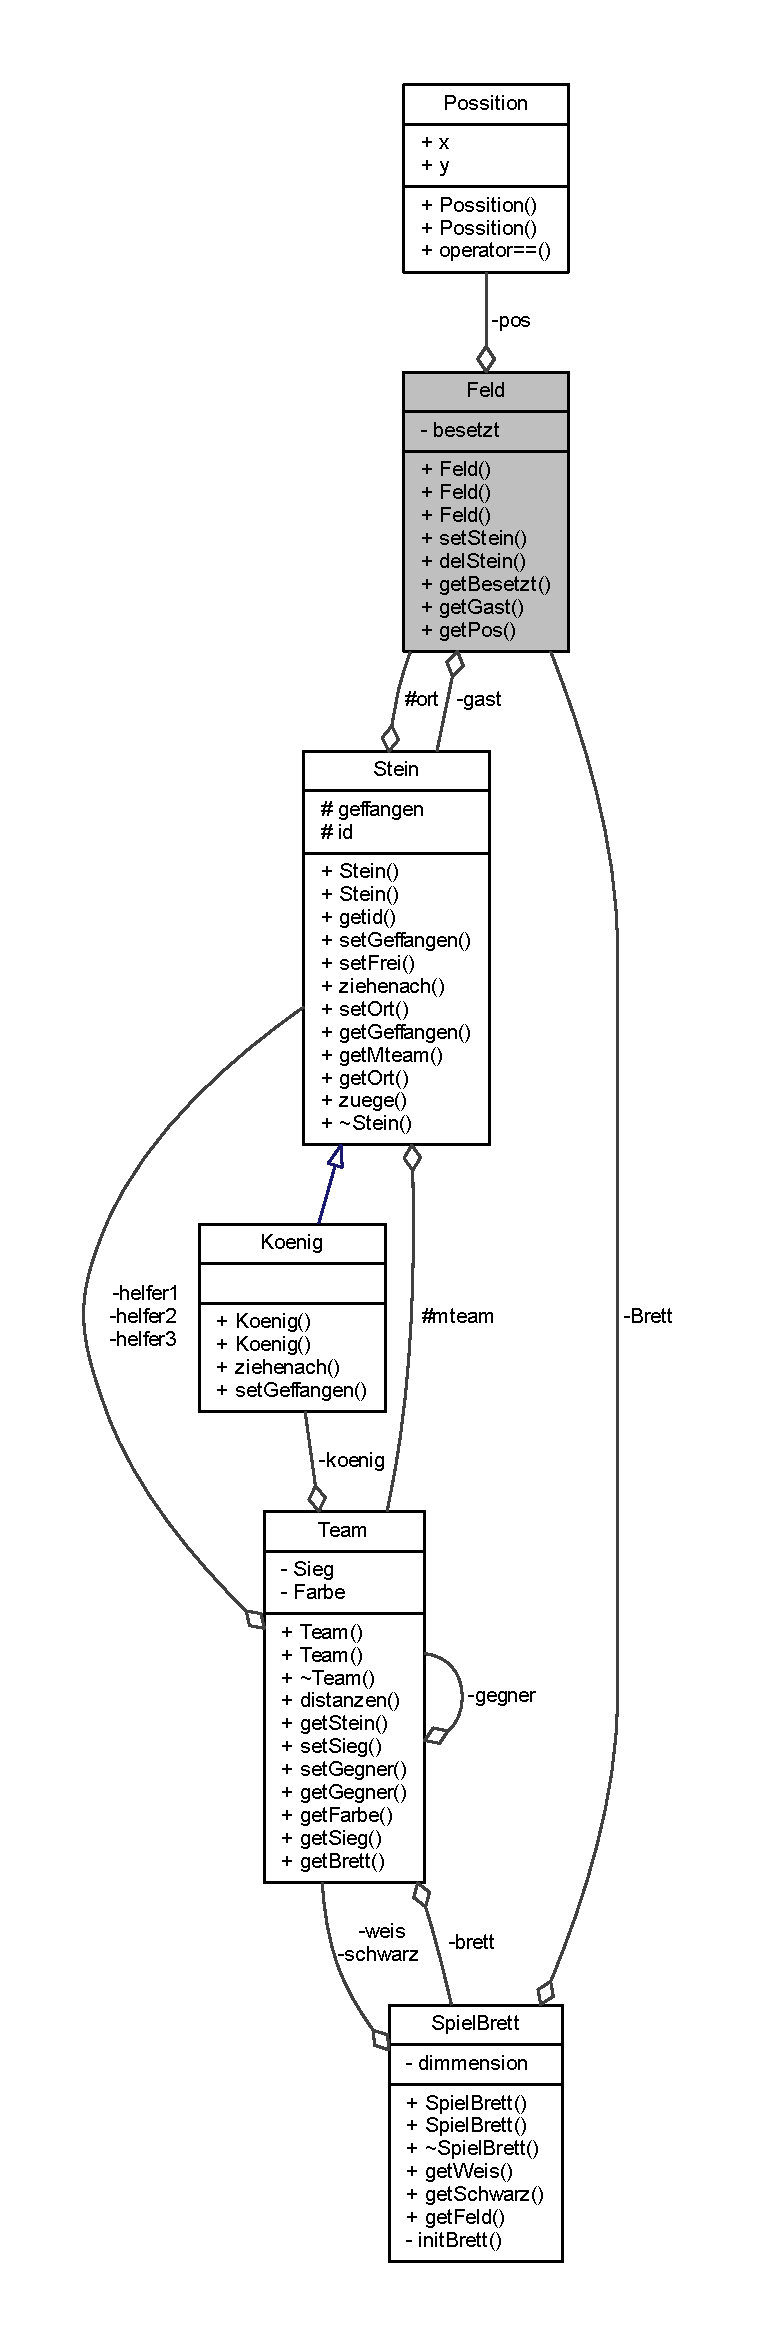
\includegraphics[height=550pt]{class_feld__coll__graph}
\end{center}
\end{figure}
\subsection*{Öffentliche Methoden}
\begin{DoxyCompactItemize}
\item 
\hyperlink{class_feld_a8a3098df53c8ae2ef988d0d2e34be1db}{Feld} ()
\item 
\hyperlink{class_feld_a5305572f4799035e118ff6c5e87df7f3}{Feld} (short nx, short ny)
\item 
\hyperlink{class_feld_a6594ff1a9881daa807483ea3754e16d0}{Feld} (\hyperlink{class_feld}{Feld} \&f)
\item 
void \hyperlink{class_feld_a00d3eec0ced82a8aee97de9b5f030df2}{set\+Stein} (\hyperlink{class_stein}{Stein} $\ast$newstein)
\item 
void \hyperlink{class_feld_a6bb4ad9a5e5ba0b7c50e43b149535a5c}{del\+Stein} ()
\item 
bool \hyperlink{class_feld_a70456d20a55214db1af93ccab6d192cd}{get\+Besetzt} ()
\item 
\hyperlink{class_stein}{Stein} $\ast$ \hyperlink{class_feld_a41f1e0c497b688ac87d6ab95c9b4914d}{get\+Gast} ()
\item 
\hyperlink{struct_possition}{Possition} \hyperlink{class_feld_adaeedb54cddaa27a5081237b60389bd3}{get\+Pos} ()
\end{DoxyCompactItemize}
\subsection*{Private Attribute}
\begin{DoxyCompactItemize}
\item 
bool \hyperlink{class_feld_aae4074e0032cce9eb0162394c639a4a0}{besetzt}
\item 
\hyperlink{struct_possition}{Possition} \hyperlink{class_feld_a1ac2c5d077b149682a32a238aec77991}{pos}
\item 
\hyperlink{class_stein}{Stein} $\ast$ \hyperlink{class_feld_a95773640265709ae8632d6a91655575d}{gast} =nullptr
\end{DoxyCompactItemize}


\subsection{Ausführliche Beschreibung}
class \hyperlink{class_feld}{Feld} Diese Klasse Symbolisiert ein \hyperlink{class_feld}{Feld} auf einem Spielbrett. 

\subsection{Beschreibung der Konstruktoren und Destruktoren}
\hypertarget{class_feld_a8a3098df53c8ae2ef988d0d2e34be1db}{}\index{Feld@{Feld}!Feld@{Feld}}
\index{Feld@{Feld}!Feld@{Feld}}
\subsubsection[{Feld}]{\setlength{\rightskip}{0pt plus 5cm}Feld\+::\+Feld (
\begin{DoxyParamCaption}
{}
\end{DoxyParamCaption}
)}\label{class_feld_a8a3098df53c8ae2ef988d0d2e34be1db}
\hypertarget{class_feld_a5305572f4799035e118ff6c5e87df7f3}{}\index{Feld@{Feld}!Feld@{Feld}}
\index{Feld@{Feld}!Feld@{Feld}}
\subsubsection[{Feld}]{\setlength{\rightskip}{0pt plus 5cm}Feld\+::\+Feld (
\begin{DoxyParamCaption}
\item[{short}]{nx, }
\item[{short}]{ny}
\end{DoxyParamCaption}
)}\label{class_feld_a5305572f4799035e118ff6c5e87df7f3}
\hyperlink{class_feld}{Feld} Konstruktor 
\begin{DoxyParams}[1]{Parameter}
\mbox{\tt in}  & {\em nx} & x Koordinaten des Feldes \\
\hline
\mbox{\tt in}  & {\em ny} & y Koordinaten des Feldes \\
\hline
\end{DoxyParams}
\hypertarget{class_feld_a6594ff1a9881daa807483ea3754e16d0}{}\index{Feld@{Feld}!Feld@{Feld}}
\index{Feld@{Feld}!Feld@{Feld}}
\subsubsection[{Feld}]{\setlength{\rightskip}{0pt plus 5cm}Feld\+::\+Feld (
\begin{DoxyParamCaption}
\item[{{\bf Feld} \&}]{f}
\end{DoxyParamCaption}
)}\label{class_feld_a6594ff1a9881daa807483ea3754e16d0}


\subsection{Dokumentation der Elementfunktionen}
\hypertarget{class_feld_a6bb4ad9a5e5ba0b7c50e43b149535a5c}{}\index{Feld@{Feld}!del\+Stein@{del\+Stein}}
\index{del\+Stein@{del\+Stein}!Feld@{Feld}}
\subsubsection[{del\+Stein}]{\setlength{\rightskip}{0pt plus 5cm}void Feld\+::del\+Stein (
\begin{DoxyParamCaption}
{}
\end{DoxyParamCaption}
)}\label{class_feld_a6bb4ad9a5e5ba0b7c50e43b149535a5c}
del\+Stein Loescht Zeiger auf Gast Setzt besetzt auf false   \hypertarget{class_feld_a70456d20a55214db1af93ccab6d192cd}{}\index{Feld@{Feld}!get\+Besetzt@{get\+Besetzt}}
\index{get\+Besetzt@{get\+Besetzt}!Feld@{Feld}}
\subsubsection[{get\+Besetzt}]{\setlength{\rightskip}{0pt plus 5cm}bool Feld\+::get\+Besetzt (
\begin{DoxyParamCaption}
{}
\end{DoxyParamCaption}
)}\label{class_feld_a70456d20a55214db1af93ccab6d192cd}
Get the value of besetzt. \begin{DoxyReturn}{Rückgabe}
the value of besetzt. 
\end{DoxyReturn}
\hypertarget{class_feld_a41f1e0c497b688ac87d6ab95c9b4914d}{}\index{Feld@{Feld}!get\+Gast@{get\+Gast}}
\index{get\+Gast@{get\+Gast}!Feld@{Feld}}
\subsubsection[{get\+Gast}]{\setlength{\rightskip}{0pt plus 5cm}{\bf Stein} $\ast$ Feld\+::get\+Gast (
\begin{DoxyParamCaption}
{}
\end{DoxyParamCaption}
)}\label{class_feld_a41f1e0c497b688ac87d6ab95c9b4914d}
get\+Gast \begin{DoxyReturn}{Rückgabe}
Gibt einen Pointer auf den Gast zurueck. 
\end{DoxyReturn}
\hypertarget{class_feld_adaeedb54cddaa27a5081237b60389bd3}{}\index{Feld@{Feld}!get\+Pos@{get\+Pos}}
\index{get\+Pos@{get\+Pos}!Feld@{Feld}}
\subsubsection[{get\+Pos}]{\setlength{\rightskip}{0pt plus 5cm}{\bf Possition} Feld\+::get\+Pos (
\begin{DoxyParamCaption}
{}
\end{DoxyParamCaption}
)}\label{class_feld_adaeedb54cddaa27a5081237b60389bd3}
get\+Pos \begin{DoxyReturn}{Rückgabe}
the value of pos. 
\end{DoxyReturn}
\hypertarget{class_feld_a00d3eec0ced82a8aee97de9b5f030df2}{}\index{Feld@{Feld}!set\+Stein@{set\+Stein}}
\index{set\+Stein@{set\+Stein}!Feld@{Feld}}
\subsubsection[{set\+Stein}]{\setlength{\rightskip}{0pt plus 5cm}void Feld\+::set\+Stein (
\begin{DoxyParamCaption}
\item[{{\bf Stein} $\ast$}]{newstein}
\end{DoxyParamCaption}
)}\label{class_feld_a00d3eec0ced82a8aee97de9b5f030df2}
Setzt \hyperlink{class_stein}{Stein} auf das \hyperlink{class_feld}{Feld} und Markiert das \hyperlink{class_feld}{Feld} als Besetzt. Falls das \hyperlink{class_feld}{Feld} besetzt ist, werden die Gaeste/\+Steine getauscht. 
\begin{DoxyParams}{Parameter}
{\em \mbox{[}in/out\mbox{]}} & $\ast$newstein pointer auf den zu setzenden \hyperlink{class_stein}{Stein}.   \\
\hline
\end{DoxyParams}


Hier ist ein Graph, der zeigt, was diese Funktion aufruft\+:\nopagebreak
\begin{figure}[H]
\begin{center}
\leavevmode
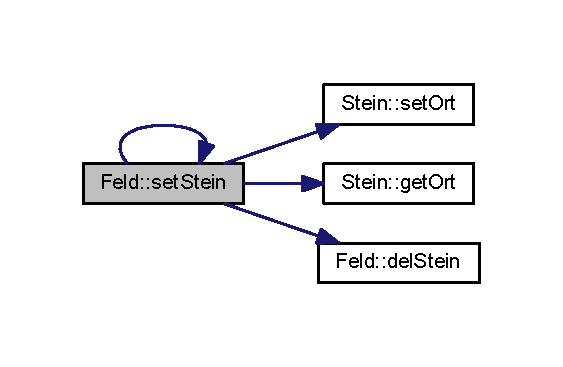
\includegraphics[width=270pt]{class_feld_a00d3eec0ced82a8aee97de9b5f030df2_cgraph}
\end{center}
\end{figure}




\subsection{Dokumentation der Datenelemente}
\hypertarget{class_feld_aae4074e0032cce9eb0162394c639a4a0}{}\index{Feld@{Feld}!besetzt@{besetzt}}
\index{besetzt@{besetzt}!Feld@{Feld}}
\subsubsection[{besetzt}]{\setlength{\rightskip}{0pt plus 5cm}bool Feld\+::besetzt\hspace{0.3cm}{\ttfamily [private]}}\label{class_feld_aae4074e0032cce9eb0162394c639a4a0}
\hypertarget{class_feld_a95773640265709ae8632d6a91655575d}{}\index{Feld@{Feld}!gast@{gast}}
\index{gast@{gast}!Feld@{Feld}}
\subsubsection[{gast}]{\setlength{\rightskip}{0pt plus 5cm}{\bf Stein}$\ast$ Feld\+::gast =nullptr\hspace{0.3cm}{\ttfamily [private]}}\label{class_feld_a95773640265709ae8632d6a91655575d}
\hypertarget{class_feld_a1ac2c5d077b149682a32a238aec77991}{}\index{Feld@{Feld}!pos@{pos}}
\index{pos@{pos}!Feld@{Feld}}
\subsubsection[{pos}]{\setlength{\rightskip}{0pt plus 5cm}{\bf Possition} Feld\+::pos\hspace{0.3cm}{\ttfamily [private]}}\label{class_feld_a1ac2c5d077b149682a32a238aec77991}


Die Dokumentation für diese Klasse wurde erzeugt aufgrund der Dateien\+:\begin{DoxyCompactItemize}
\item 
\hyperlink{_feld_8h}{Feld.\+h}\item 
\hyperlink{_feld_8cpp}{Feld.\+cpp}\end{DoxyCompactItemize}

\hypertarget{class_g_u_i}{}\section{G\+U\+I Klassenreferenz}
\label{class_g_u_i}\index{G\+U\+I@{G\+U\+I}}


{\ttfamily \#include $<$G\+U\+I.\+h$>$}



Zusammengehörigkeiten von G\+U\+I\+:\nopagebreak
\begin{figure}[H]
\begin{center}
\leavevmode
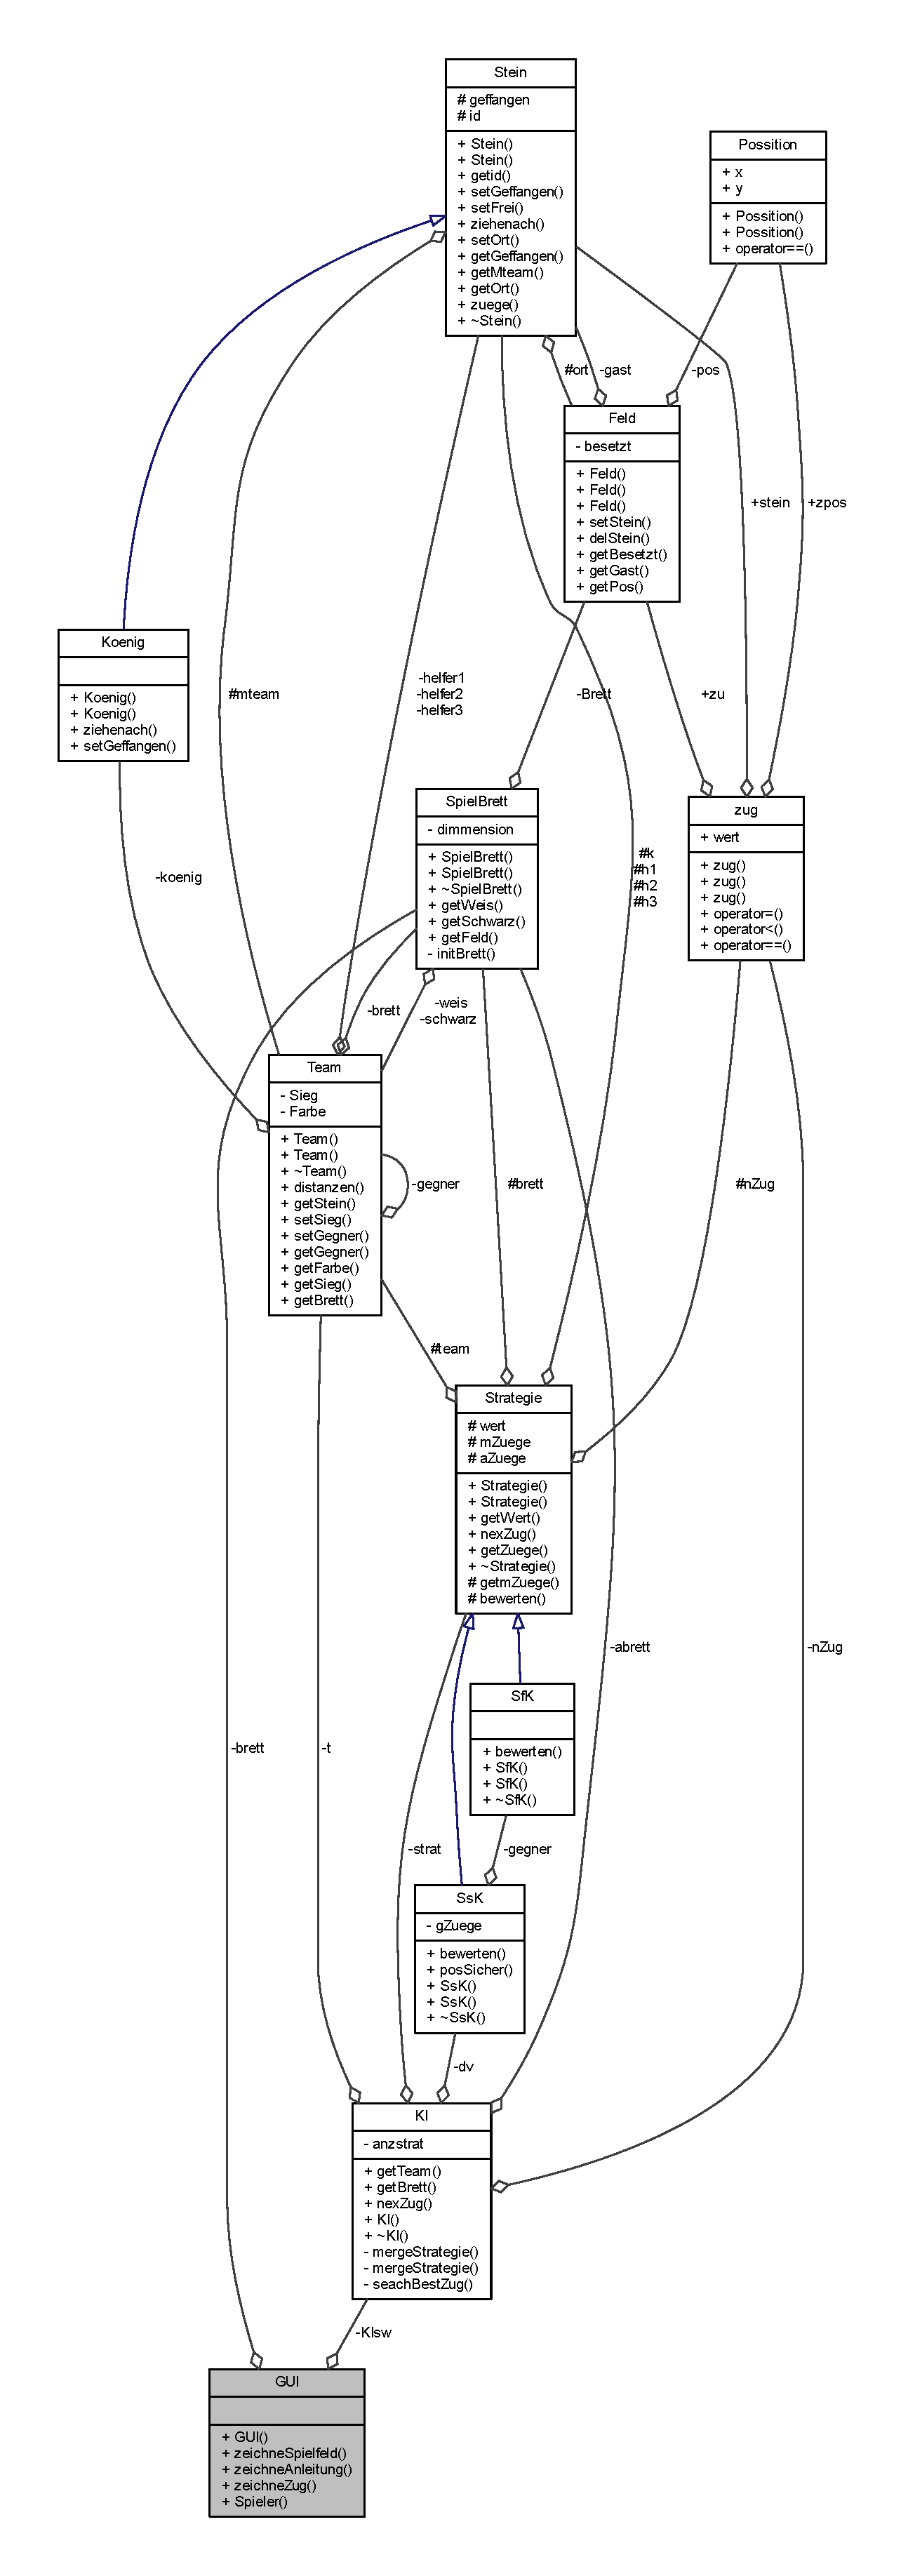
\includegraphics[height=550pt]{class_g_u_i__coll__graph}
\end{center}
\end{figure}
\subsection*{Öffentliche Methoden}
\begin{DoxyCompactItemize}
\item 
\hyperlink{class_g_u_i_abdb64f04f2492fbe458a9585265457ed}{G\+U\+I} (\hyperlink{class_spiel_brett}{Spiel\+Brett} $\ast$br, \hyperlink{class_k_i}{K\+I} $\ast$ki)
\item 
void \hyperlink{class_g_u_i_a3c4186a30634b02fadf9088478fcd6d8}{zeichne\+Spielfeld} (int \hyperlink{structzug}{zug}, int spieler)
\item 
void \hyperlink{class_g_u_i_ab679c856cec515619230cfc070b620a4}{zeichne\+Anleitung} ()
\item 
void \hyperlink{class_g_u_i_ab892cc67dca7bd80350101493dd26542}{zeichne\+Zug} (int \hyperlink{structzug}{zug}, int spieler, int zeile, int spalte)
\item 
void \hyperlink{class_g_u_i_a96e74958db22ad7359287eb2e06d0cb2}{Spieler} (bool farbe, int \hyperlink{structzug}{zug}, int spieler)
\end{DoxyCompactItemize}
\subsection*{Private Attribute}
\begin{DoxyCompactItemize}
\item 
\hyperlink{class_spiel_brett}{Spiel\+Brett} $\ast$ \hyperlink{class_g_u_i_ad27ec30e361c6b18ba0b03f4eb3c2697}{brett}
\item 
\hyperlink{class_k_i}{K\+I} $\ast$ \hyperlink{class_g_u_i_a859788c2a71895514783423c305cf886}{K\+Isw}
\end{DoxyCompactItemize}


\subsection{Ausführliche Beschreibung}
class \hyperlink{class_g_u_i}{G\+U\+I} Die Abkürzung \hyperlink{class_g_u_i}{G\+U\+I} steht für graphical user interface bzw. grafische Benutzeroberfläche. Durch diese Klasse wird dem Benutzer eine grafische Oberfläche zur Verfügung gestellt, über die er mit dem Programm interagierien kann. Alle Benutzereingaben erfolgen ausschließlich über die Tastatur. Unterstützend wird die Strucktur der erwarteten Eingabe in Klammern mit angegeben. Sollte dennoch der Benutzer eine Falsch Eingabe tätigen, so wird er darauf hingewiesen und kann seine Eingabe nach 3 Sekunken wiederholen. Die Darstellung des Spielfeldes und wichtiger Spielparameter erfolgt in der Windows Konsole über A\+N\+S\+I-\/\+Zeichen. 

\subsection{Beschreibung der Konstruktoren und Destruktoren}
\hypertarget{class_g_u_i_abdb64f04f2492fbe458a9585265457ed}{}\index{G\+U\+I@{G\+U\+I}!G\+U\+I@{G\+U\+I}}
\index{G\+U\+I@{G\+U\+I}!G\+U\+I@{G\+U\+I}}
\subsubsection[{G\+U\+I}]{\setlength{\rightskip}{0pt plus 5cm}G\+U\+I\+::\+G\+U\+I (
\begin{DoxyParamCaption}
\item[{{\bf Spiel\+Brett} $\ast$}]{br, }
\item[{{\bf K\+I} $\ast$}]{ki}
\end{DoxyParamCaption}
)}\label{class_g_u_i_abdb64f04f2492fbe458a9585265457ed}


\subsection{Dokumentation der Elementfunktionen}
\hypertarget{class_g_u_i_a96e74958db22ad7359287eb2e06d0cb2}{}\index{G\+U\+I@{G\+U\+I}!Spieler@{Spieler}}
\index{Spieler@{Spieler}!G\+U\+I@{G\+U\+I}}
\subsubsection[{Spieler}]{\setlength{\rightskip}{0pt plus 5cm}void G\+U\+I\+::\+Spieler (
\begin{DoxyParamCaption}
\item[{bool}]{farbe, }
\item[{int}]{zug, }
\item[{int}]{spieler}
\end{DoxyParamCaption}
)}\label{class_g_u_i_a96e74958db22ad7359287eb2e06d0cb2}
zeichne\+Zug(zug,spieler,zeile,spalte) Mit dieser Funktion wird dem Spieler alle zulässigen Züge des ausgewählten Steins angezeigt.


\begin{DoxyParams}{Parameter}
{\em \mbox{[}int\mbox{]}} & zug gibt den aktuellen Zug an \\
\hline
{\em \mbox{[}int\mbox{]}} & spieler gibt an, welcher Spieler gerade am Zug ist \\
\hline
{\em \mbox{[}int\mbox{]}} & zeile Zeile des ausgewählten Steins \\
\hline
{\em \mbox{[}int\mbox{]}} & spalte Spalte des ausgewählten Steins\\
\hline
\end{DoxyParams}
  \hypertarget{class_g_u_i_ab679c856cec515619230cfc070b620a4}{}\index{G\+U\+I@{G\+U\+I}!zeichne\+Anleitung@{zeichne\+Anleitung}}
\index{zeichne\+Anleitung@{zeichne\+Anleitung}!G\+U\+I@{G\+U\+I}}
\subsubsection[{zeichne\+Anleitung}]{\setlength{\rightskip}{0pt plus 5cm}void G\+U\+I\+::zeichne\+Anleitung (
\begin{DoxyParamCaption}
{}
\end{DoxyParamCaption}
)}\label{class_g_u_i_ab679c856cec515619230cfc070b620a4}
zeichne\+Spielfeld(zug,spieler) Mit dieser Funktion wird das Spielfeld grafisch für den Spieler aufbereitet. 
\begin{DoxyParams}{Parameter}
{\em \mbox{[}int\mbox{]}} & zug gibt den aktuelle Zug an \\
\hline
{\em \mbox{[}int\mbox{]}} & spieler gibt an, welcher Spieler an Zug ist\\
\hline
\end{DoxyParams}
  \hypertarget{class_g_u_i_a3c4186a30634b02fadf9088478fcd6d8}{}\index{G\+U\+I@{G\+U\+I}!zeichne\+Spielfeld@{zeichne\+Spielfeld}}
\index{zeichne\+Spielfeld@{zeichne\+Spielfeld}!G\+U\+I@{G\+U\+I}}
\subsubsection[{zeichne\+Spielfeld}]{\setlength{\rightskip}{0pt plus 5cm}void G\+U\+I\+::zeichne\+Spielfeld (
\begin{DoxyParamCaption}
\item[{int}]{zug, }
\item[{int}]{spieler}
\end{DoxyParamCaption}
)}\label{class_g_u_i_a3c4186a30634b02fadf9088478fcd6d8}
\hyperlink{class_g_u_i}{G\+U\+I} Diese Funktion ist ein Konstructor für eine Instanz von der Klasse Spielbrett. \hypertarget{class_g_u_i_ab892cc67dca7bd80350101493dd26542}{}\index{G\+U\+I@{G\+U\+I}!zeichne\+Zug@{zeichne\+Zug}}
\index{zeichne\+Zug@{zeichne\+Zug}!G\+U\+I@{G\+U\+I}}
\subsubsection[{zeichne\+Zug}]{\setlength{\rightskip}{0pt plus 5cm}void G\+U\+I\+::zeichne\+Zug (
\begin{DoxyParamCaption}
\item[{int}]{zug, }
\item[{int}]{spieler, }
\item[{int}]{zeile, }
\item[{int}]{spalte}
\end{DoxyParamCaption}
)}\label{class_g_u_i_ab892cc67dca7bd80350101493dd26542}
zeichen\+Anleitung() Diese Funktion gibt dem Benutzer Auskunft über die Spielregeln.

  

\subsection{Dokumentation der Datenelemente}
\hypertarget{class_g_u_i_ad27ec30e361c6b18ba0b03f4eb3c2697}{}\index{G\+U\+I@{G\+U\+I}!brett@{brett}}
\index{brett@{brett}!G\+U\+I@{G\+U\+I}}
\subsubsection[{brett}]{\setlength{\rightskip}{0pt plus 5cm}{\bf Spiel\+Brett}$\ast$ G\+U\+I\+::brett\hspace{0.3cm}{\ttfamily [private]}}\label{class_g_u_i_ad27ec30e361c6b18ba0b03f4eb3c2697}
\hypertarget{class_g_u_i_a859788c2a71895514783423c305cf886}{}\index{G\+U\+I@{G\+U\+I}!K\+Isw@{K\+Isw}}
\index{K\+Isw@{K\+Isw}!G\+U\+I@{G\+U\+I}}
\subsubsection[{K\+Isw}]{\setlength{\rightskip}{0pt plus 5cm}{\bf K\+I}$\ast$ G\+U\+I\+::\+K\+Isw\hspace{0.3cm}{\ttfamily [private]}}\label{class_g_u_i_a859788c2a71895514783423c305cf886}


Die Dokumentation für diese Klasse wurde erzeugt aufgrund der Dateien\+:\begin{DoxyCompactItemize}
\item 
\hyperlink{_g_u_i_8h}{G\+U\+I.\+h}\item 
\hyperlink{_g_u_i_8cpp}{G\+U\+I.\+cpp}\end{DoxyCompactItemize}

\hypertarget{class_k_i}{}\section{K\+I Klassenreferenz}
\label{class_k_i}\index{K\+I@{K\+I}}


{\ttfamily \#include $<$K\+I.\+h$>$}



Zusammengehörigkeiten von K\+I\+:\nopagebreak
\begin{figure}[H]
\begin{center}
\leavevmode
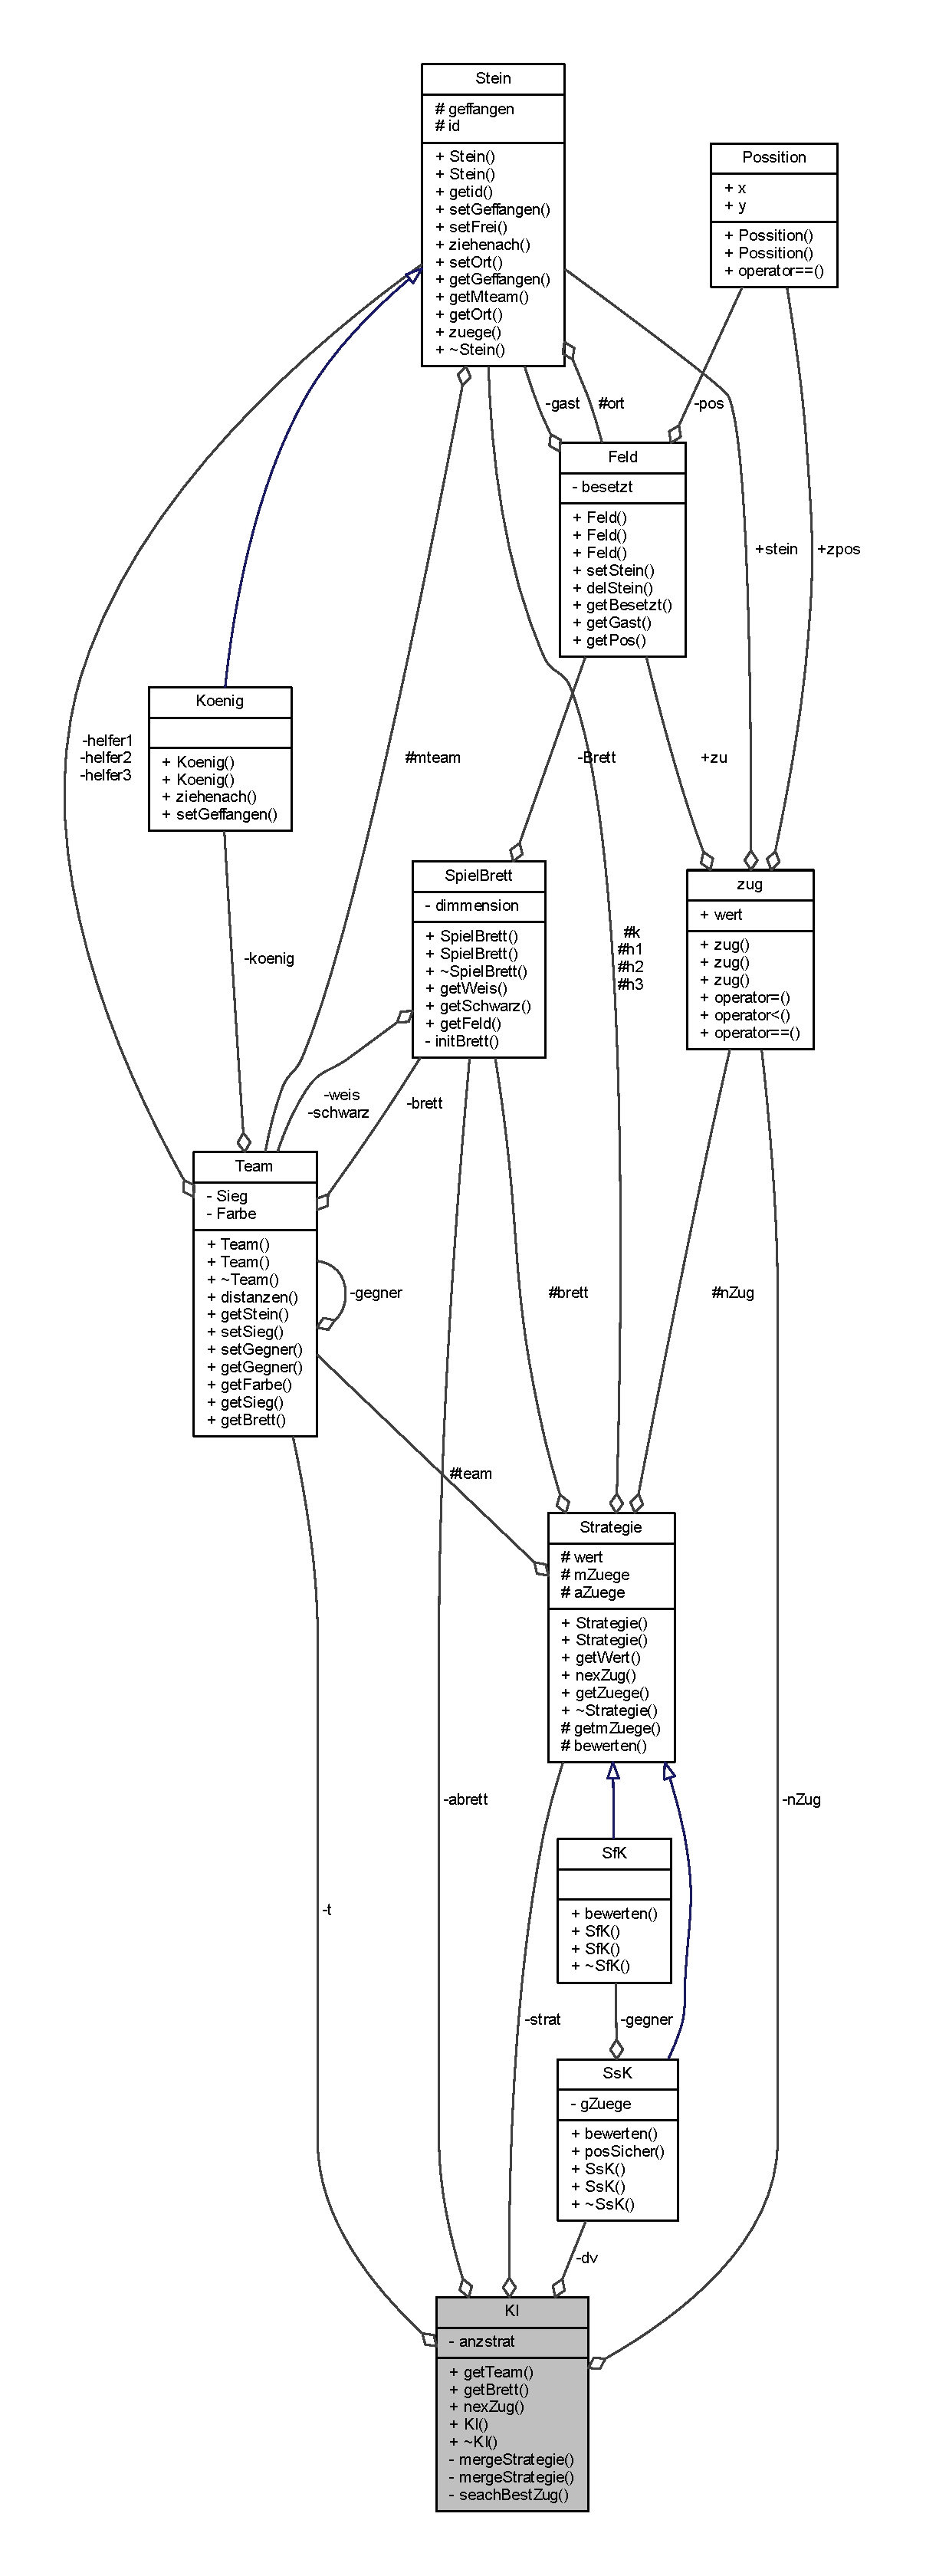
\includegraphics[height=550pt]{class_k_i__coll__graph}
\end{center}
\end{figure}
\subsection*{Öffentliche Methoden}
\begin{DoxyCompactItemize}
\item 
\hyperlink{class_team}{Team} \& \hyperlink{class_k_i_a731391b304aaf237500db42f8dee4690}{get\+Team} ()
\item 
\hyperlink{class_spiel_brett}{Spiel\+Brett} \& \hyperlink{class_k_i_a204bc5eb350c5d7cfc5f7e56fff9690c}{get\+Brett} ()
\item 
void \hyperlink{class_k_i_a840820c024ad7069c2064fc30f964169}{nex\+Zug} ()
\item 
\hyperlink{class_k_i_aa3c0a5eadcdf9c5fee6d8180dac17d0a}{K\+I} (\hyperlink{class_team}{Team} \&\hyperlink{class_k_i_a611b37548d94d9dce7e68024aa943733}{t})
\item 
virtual \hyperlink{class_k_i_afd1109cfccff505f519d60d9958efad9}{$\sim$\+K\+I} ()
\end{DoxyCompactItemize}
\subsection*{Private Methoden}
\begin{DoxyCompactItemize}
\item 
std\+::vector$<$ \hyperlink{structzug}{zug} $>$ \hyperlink{class_k_i_af4bec8491d051702c49d780a25feb1cb}{merge\+Strategie} (\hyperlink{class_strategie}{Strategie} $\ast$st1, std\+::vector$<$ \hyperlink{structzug}{zug} $>$ st2\+Zuege)
\item 
std\+::vector$<$ \hyperlink{structzug}{zug} $>$ \hyperlink{class_k_i_ae97a6dd7ab3de2a934ca5c28c4cc63b3}{merge\+Strategie} (\hyperlink{class_strategie}{Strategie} $\ast$st1, \hyperlink{class_strategie}{Strategie} $\ast$st2)
\item 
void \hyperlink{class_k_i_afa90fdb068e7b06e58db40b1ceeb8216}{seach\+Best\+Zug} ()
\end{DoxyCompactItemize}
\subsection*{Private Attribute}
\begin{DoxyCompactItemize}
\item 
\hyperlink{class_team}{Team} \& \hyperlink{class_k_i_a611b37548d94d9dce7e68024aa943733}{t}
\item 
\hyperlink{class_spiel_brett}{Spiel\+Brett} \& \hyperlink{class_k_i_a93f7368fa6746ddb1e51d804ddaea096}{abrett}
\item 
\hyperlink{class_strategie}{Strategie} $\ast$ \hyperlink{class_k_i_a6e07007b67f0a2778de3148ed5612921}{strat} \mbox{[}\hyperlink{class_k_i_a16d7b067120b9b638781d5e5e6dcc005}{anzstrat}\mbox{]}
\item 
\hyperlink{class_ss_k}{Ss\+K} $\ast$ \hyperlink{class_k_i_a34cb945060f752556a068ccf1771c531}{dv}
\item 
\hyperlink{structzug}{zug} \hyperlink{class_k_i_acfefb24fdddb36cbfe2dff9e1d5d8296}{n\+Zug}
\end{DoxyCompactItemize}
\subsection*{Statische, private Attribute}
\begin{DoxyCompactItemize}
\item 
static const int \hyperlink{class_k_i_a16d7b067120b9b638781d5e5e6dcc005}{anzstrat} =4
\end{DoxyCompactItemize}


\subsection{Ausführliche Beschreibung}
class \hyperlink{class_k_i}{K\+I} Ist eine Klasse die aus den möglichen Spielzügen den besten auswählt. Sie ist mit zusätzlichen Strategien erweiterbar. 

\subsection{Beschreibung der Konstruktoren und Destruktoren}
\hypertarget{class_k_i_aa3c0a5eadcdf9c5fee6d8180dac17d0a}{}\index{K\+I@{K\+I}!K\+I@{K\+I}}
\index{K\+I@{K\+I}!K\+I@{K\+I}}
\subsubsection[{K\+I}]{\setlength{\rightskip}{0pt plus 5cm}K\+I\+::\+K\+I (
\begin{DoxyParamCaption}
\item[{{\bf Team} \&}]{t}
\end{DoxyParamCaption}
)}\label{class_k_i_aa3c0a5eadcdf9c5fee6d8180dac17d0a}
\hyperlink{class_k_i}{K\+I} Konstruktor 
\begin{DoxyParams}[1]{Parameter}
\mbox{\tt in,out}  & {\em t} & Referenz auf das \hyperlink{class_team}{Team}, das gesteuert werden soll \\
\hline
\end{DoxyParams}
\hypertarget{class_k_i_afd1109cfccff505f519d60d9958efad9}{}\index{K\+I@{K\+I}!````~K\+I@{$\sim$\+K\+I}}
\index{````~K\+I@{$\sim$\+K\+I}!K\+I@{K\+I}}
\subsubsection[{$\sim$\+K\+I}]{\setlength{\rightskip}{0pt plus 5cm}K\+I\+::$\sim$\+K\+I (
\begin{DoxyParamCaption}
{}
\end{DoxyParamCaption}
)\hspace{0.3cm}{\ttfamily [virtual]}}\label{class_k_i_afd1109cfccff505f519d60d9958efad9}


\subsection{Dokumentation der Elementfunktionen}
\hypertarget{class_k_i_a204bc5eb350c5d7cfc5f7e56fff9690c}{}\index{K\+I@{K\+I}!get\+Brett@{get\+Brett}}
\index{get\+Brett@{get\+Brett}!K\+I@{K\+I}}
\subsubsection[{get\+Brett}]{\setlength{\rightskip}{0pt plus 5cm}{\bf Spiel\+Brett} \& K\+I\+::get\+Brett (
\begin{DoxyParamCaption}
{}
\end{DoxyParamCaption}
)}\label{class_k_i_a204bc5eb350c5d7cfc5f7e56fff9690c}
get\+Brett \begin{DoxyReturn}{Rückgabe}
Referenz auf das Spielbrett 
\end{DoxyReturn}
\hypertarget{class_k_i_a731391b304aaf237500db42f8dee4690}{}\index{K\+I@{K\+I}!get\+Team@{get\+Team}}
\index{get\+Team@{get\+Team}!K\+I@{K\+I}}
\subsubsection[{get\+Team}]{\setlength{\rightskip}{0pt plus 5cm}{\bf Team} \& K\+I\+::get\+Team (
\begin{DoxyParamCaption}
{}
\end{DoxyParamCaption}
)}\label{class_k_i_a731391b304aaf237500db42f8dee4690}
get\+Team \begin{DoxyReturn}{Rückgabe}
Referenz auf das gesteuerte \hyperlink{class_team}{Team} 
\end{DoxyReturn}
\hypertarget{class_k_i_af4bec8491d051702c49d780a25feb1cb}{}\index{K\+I@{K\+I}!merge\+Strategie@{merge\+Strategie}}
\index{merge\+Strategie@{merge\+Strategie}!K\+I@{K\+I}}
\subsubsection[{merge\+Strategie}]{\setlength{\rightskip}{0pt plus 5cm}std\+::vector$<$ {\bf zug} $>$ K\+I\+::merge\+Strategie (
\begin{DoxyParamCaption}
\item[{{\bf Strategie} $\ast$}]{st1, }
\item[{std\+::vector$<$ {\bf zug} $>$}]{st2\+Zuege}
\end{DoxyParamCaption}
)\hspace{0.3cm}{\ttfamily [private]}}\label{class_k_i_af4bec8491d051702c49d780a25feb1cb}
merge\+Strategie Vereint zwei Strategien und führt die Wertigkeiten zusammen. Je kleiner die Wertigkeits-\/\+Zahl desto besser ist der zug.  
\begin{DoxyImageNoCaption}
  \mbox{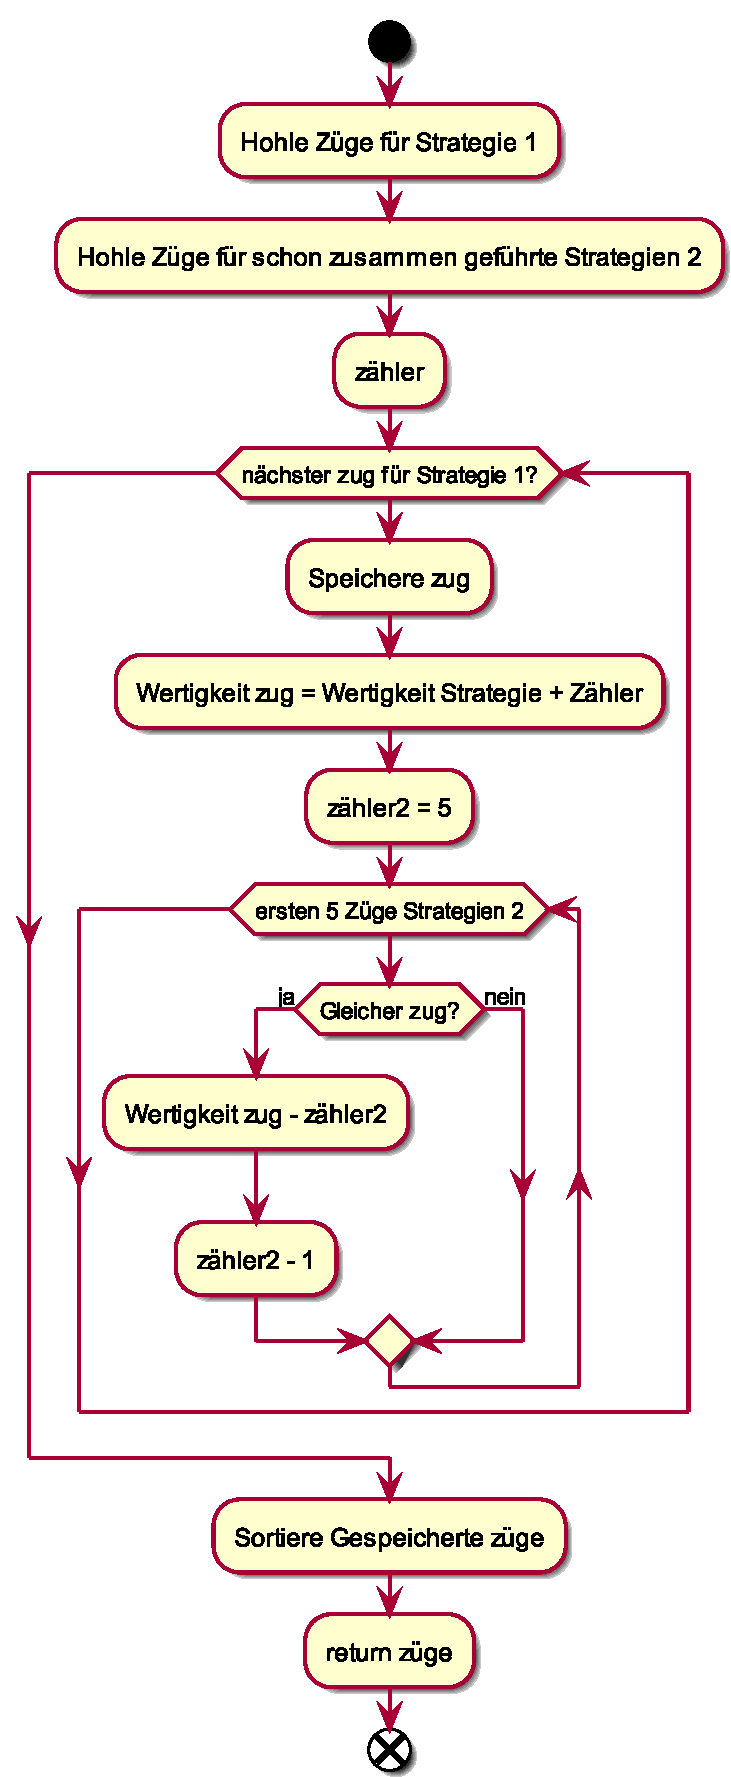
\includegraphics[width=\textwidth,height=\textheight/2,keepaspectratio=true]{KI_mergeStrategie}}
\end{DoxyImageNoCaption}
 
\begin{DoxyParams}[1]{Parameter}
\mbox{\tt in}  & {\em st1} & Pointer auf eine \hyperlink{class_strategie}{Strategie} \\
\hline
\mbox{\tt in}  & {\em st2\+Zuege} & Vector mit Zügen. \\
\hline
\end{DoxyParams}
\begin{DoxyReturn}{Rückgabe}
Vector mit nach wertigkeit sortierten zügen.  
\end{DoxyReturn}


Hier ist ein Graph, der zeigt, was diese Funktion aufruft\+:\nopagebreak
\begin{figure}[H]
\begin{center}
\leavevmode
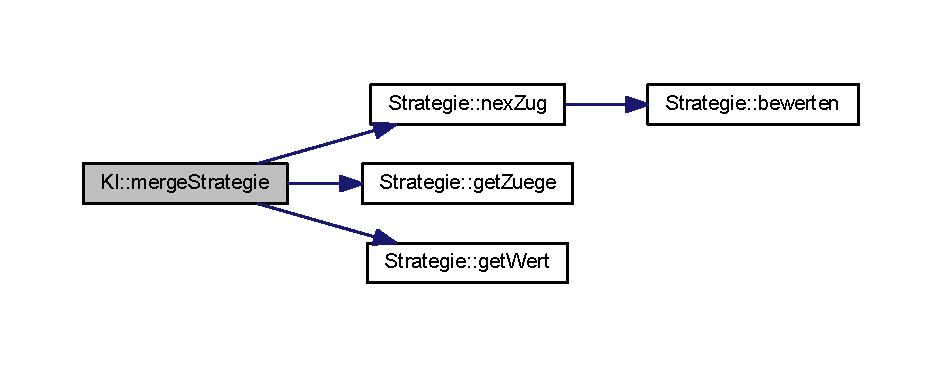
\includegraphics[width=350pt]{class_k_i_af4bec8491d051702c49d780a25feb1cb_cgraph}
\end{center}
\end{figure}


\hypertarget{class_k_i_ae97a6dd7ab3de2a934ca5c28c4cc63b3}{}\index{K\+I@{K\+I}!merge\+Strategie@{merge\+Strategie}}
\index{merge\+Strategie@{merge\+Strategie}!K\+I@{K\+I}}
\subsubsection[{merge\+Strategie}]{\setlength{\rightskip}{0pt plus 5cm}std\+::vector$<$ {\bf zug} $>$ K\+I\+::merge\+Strategie (
\begin{DoxyParamCaption}
\item[{{\bf Strategie} $\ast$}]{st1, }
\item[{{\bf Strategie} $\ast$}]{st2}
\end{DoxyParamCaption}
)\hspace{0.3cm}{\ttfamily [private]}}\label{class_k_i_ae97a6dd7ab3de2a934ca5c28c4cc63b3}

\begin{DoxyItemize}
\item merge\+Strategie Vereint zwei Strategien und fürt die Wertigkeiten zusammen. Je kleiner die wertigkeits Zahl desto besser ist der Zug.  
\begin{DoxyImageNoCaption}
  \mbox{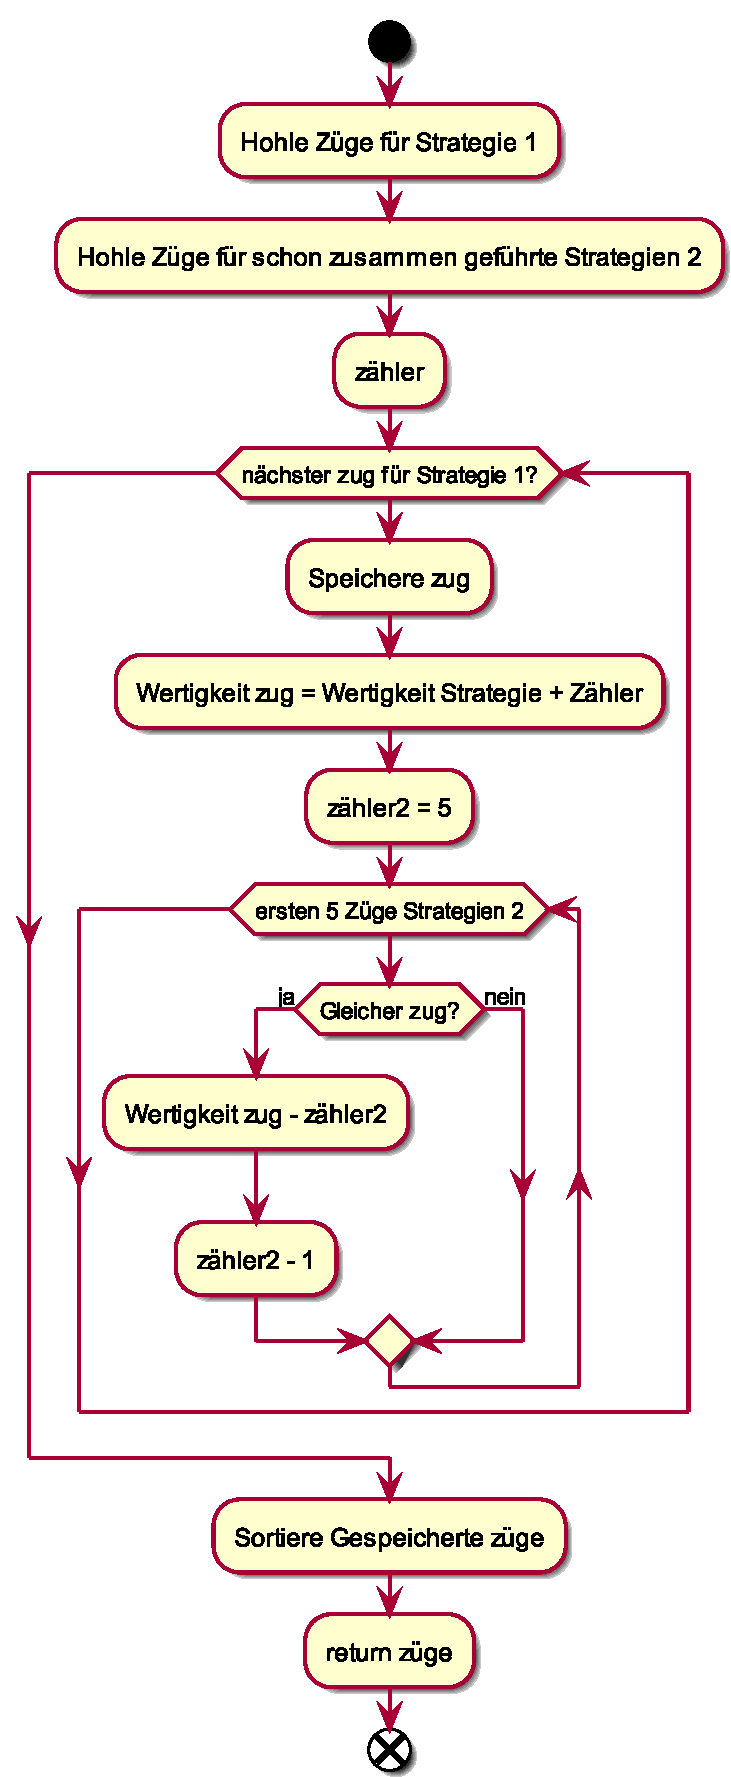
\includegraphics[width=\textwidth,height=\textheight/2,keepaspectratio=true]{KI_mergeStrategie}}
\end{DoxyImageNoCaption}
 
\begin{DoxyParams}[1]{Parameter}
\mbox{\tt in}  & {\em st1} & Pointer auf eine \hyperlink{class_strategie}{Strategie}. \\
\hline
\mbox{\tt in}  & {\em st2} & Pointer auf eine \hyperlink{class_strategie}{Strategie}. \\
\hline
\end{DoxyParams}
\begin{DoxyReturn}{Rückgabe}
Vector mit nach Wertigkeit sortierten Zügen. 
\end{DoxyReturn}

\end{DoxyItemize}

Hier ist ein Graph, der zeigt, was diese Funktion aufruft\+:\nopagebreak
\begin{figure}[H]
\begin{center}
\leavevmode
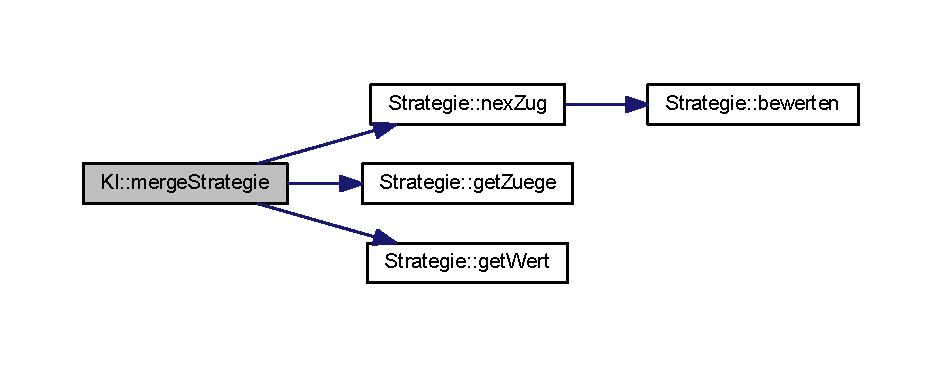
\includegraphics[width=350pt]{class_k_i_ae97a6dd7ab3de2a934ca5c28c4cc63b3_cgraph}
\end{center}
\end{figure}


\hypertarget{class_k_i_a840820c024ad7069c2064fc30f964169}{}\index{K\+I@{K\+I}!nex\+Zug@{nex\+Zug}}
\index{nex\+Zug@{nex\+Zug}!K\+I@{K\+I}}
\subsubsection[{nex\+Zug}]{\setlength{\rightskip}{0pt plus 5cm}void K\+I\+::nex\+Zug (
\begin{DoxyParamCaption}
{}
\end{DoxyParamCaption}
)}\label{class_k_i_a840820c024ad7069c2064fc30f964169}
nex\+Zug Führt den nächsten Zug aus  
\begin{DoxyImageNoCaption}
  \mbox{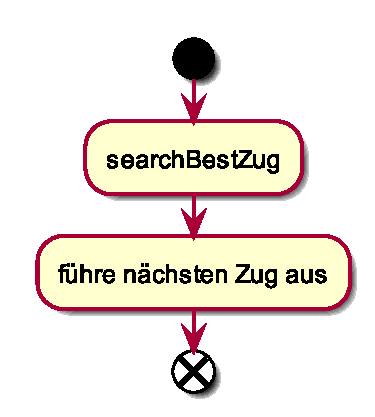
\includegraphics[width=\textwidth,height=\textheight/2,keepaspectratio=true]{KI_nexZug}}
\end{DoxyImageNoCaption}
  

Hier ist ein Graph, der zeigt, was diese Funktion aufruft\+:\nopagebreak
\begin{figure}[H]
\begin{center}
\leavevmode
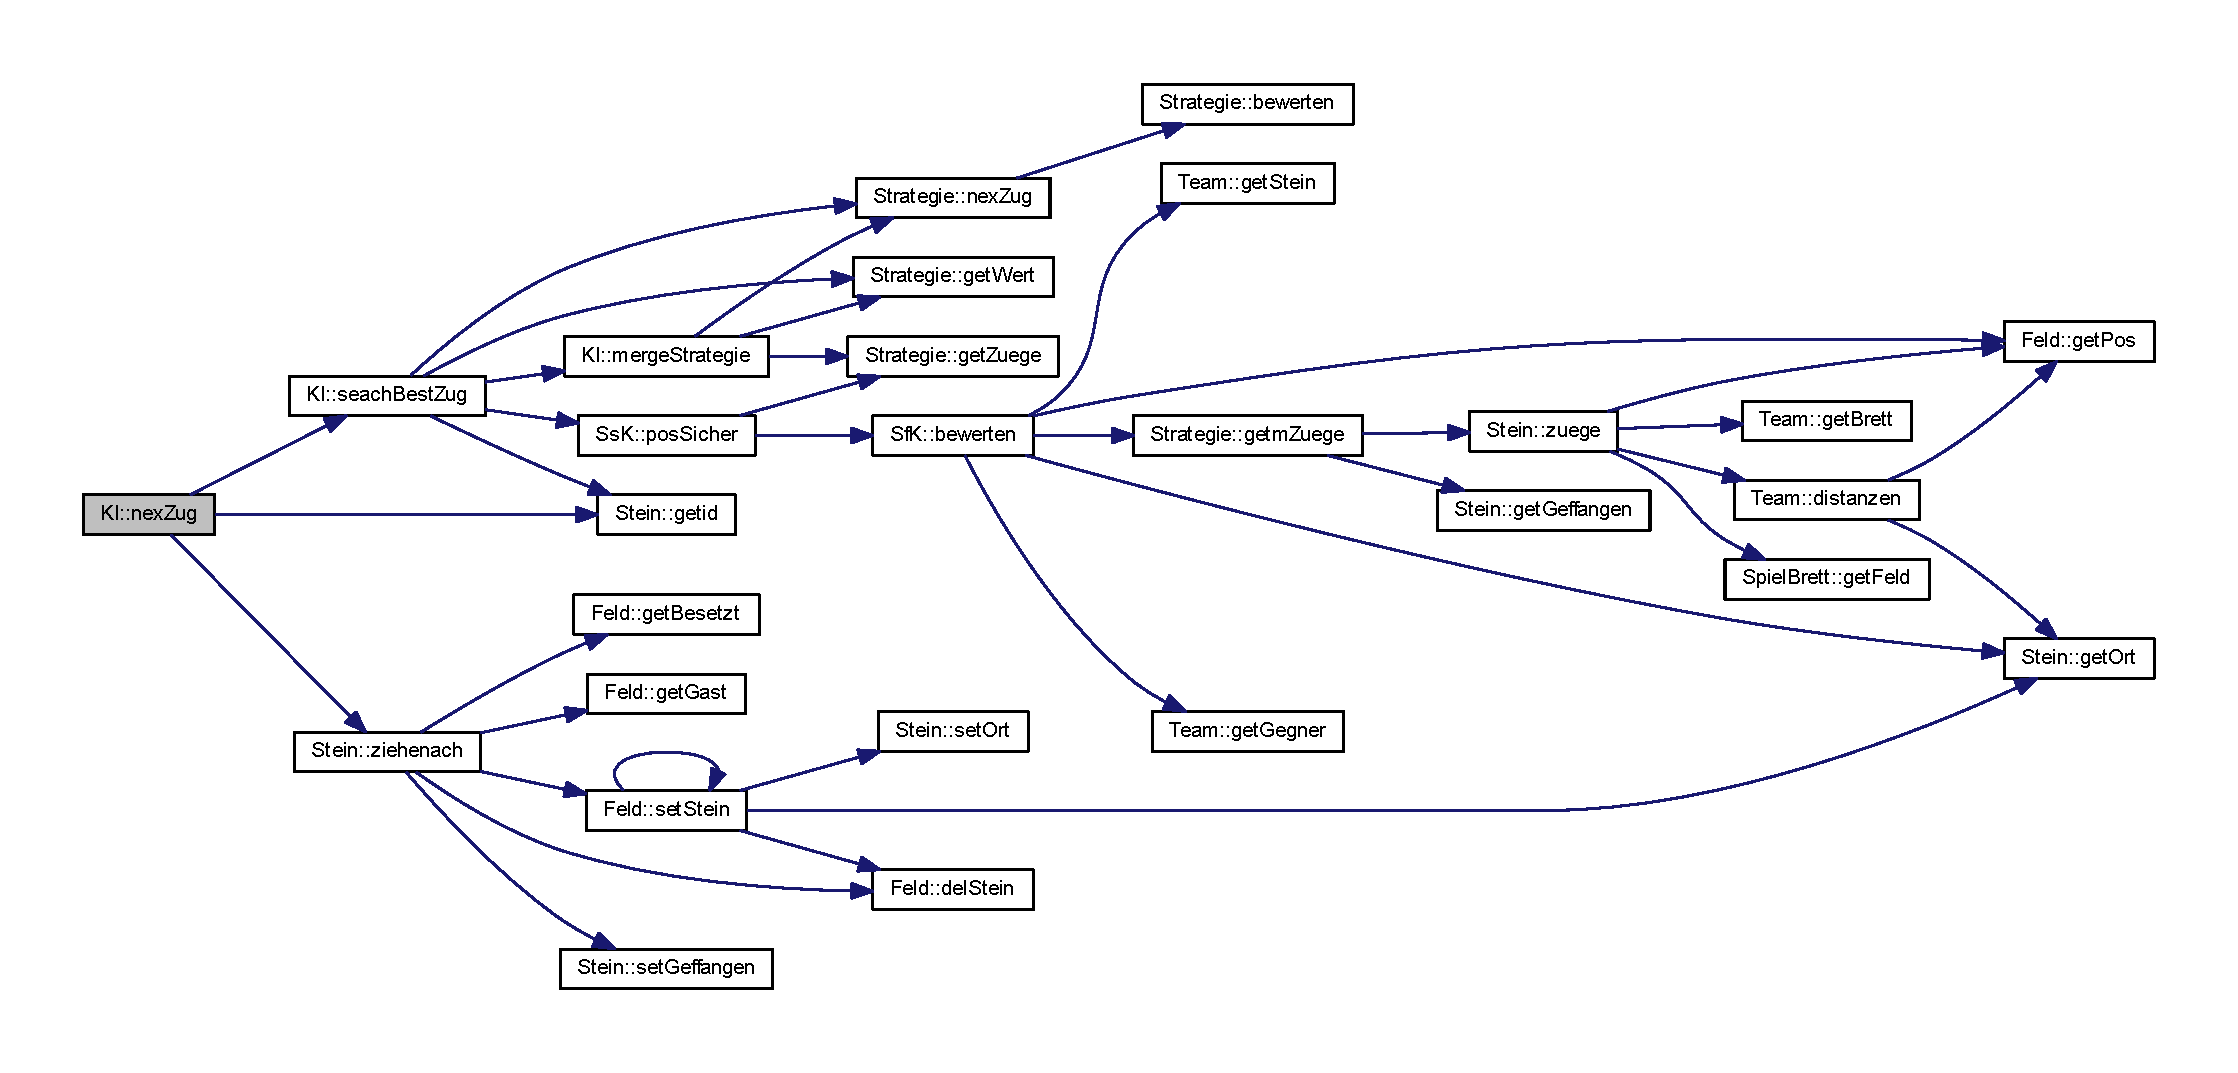
\includegraphics[width=350pt]{class_k_i_a840820c024ad7069c2064fc30f964169_cgraph}
\end{center}
\end{figure}


\hypertarget{class_k_i_afa90fdb068e7b06e58db40b1ceeb8216}{}\index{K\+I@{K\+I}!seach\+Best\+Zug@{seach\+Best\+Zug}}
\index{seach\+Best\+Zug@{seach\+Best\+Zug}!K\+I@{K\+I}}
\subsubsection[{seach\+Best\+Zug}]{\setlength{\rightskip}{0pt plus 5cm}void K\+I\+::seach\+Best\+Zug (
\begin{DoxyParamCaption}
{}
\end{DoxyParamCaption}
)\hspace{0.3cm}{\ttfamily [private]}}\label{class_k_i_afa90fdb068e7b06e58db40b1ceeb8216}
seach\+Best\+Zug Wählt aus den zusammengefürten Strategien den besten Zug aus. Und stelt sicher das der König nicht in Gefahr ist bzw. kommt.  
\begin{DoxyImageNoCaption}
  \mbox{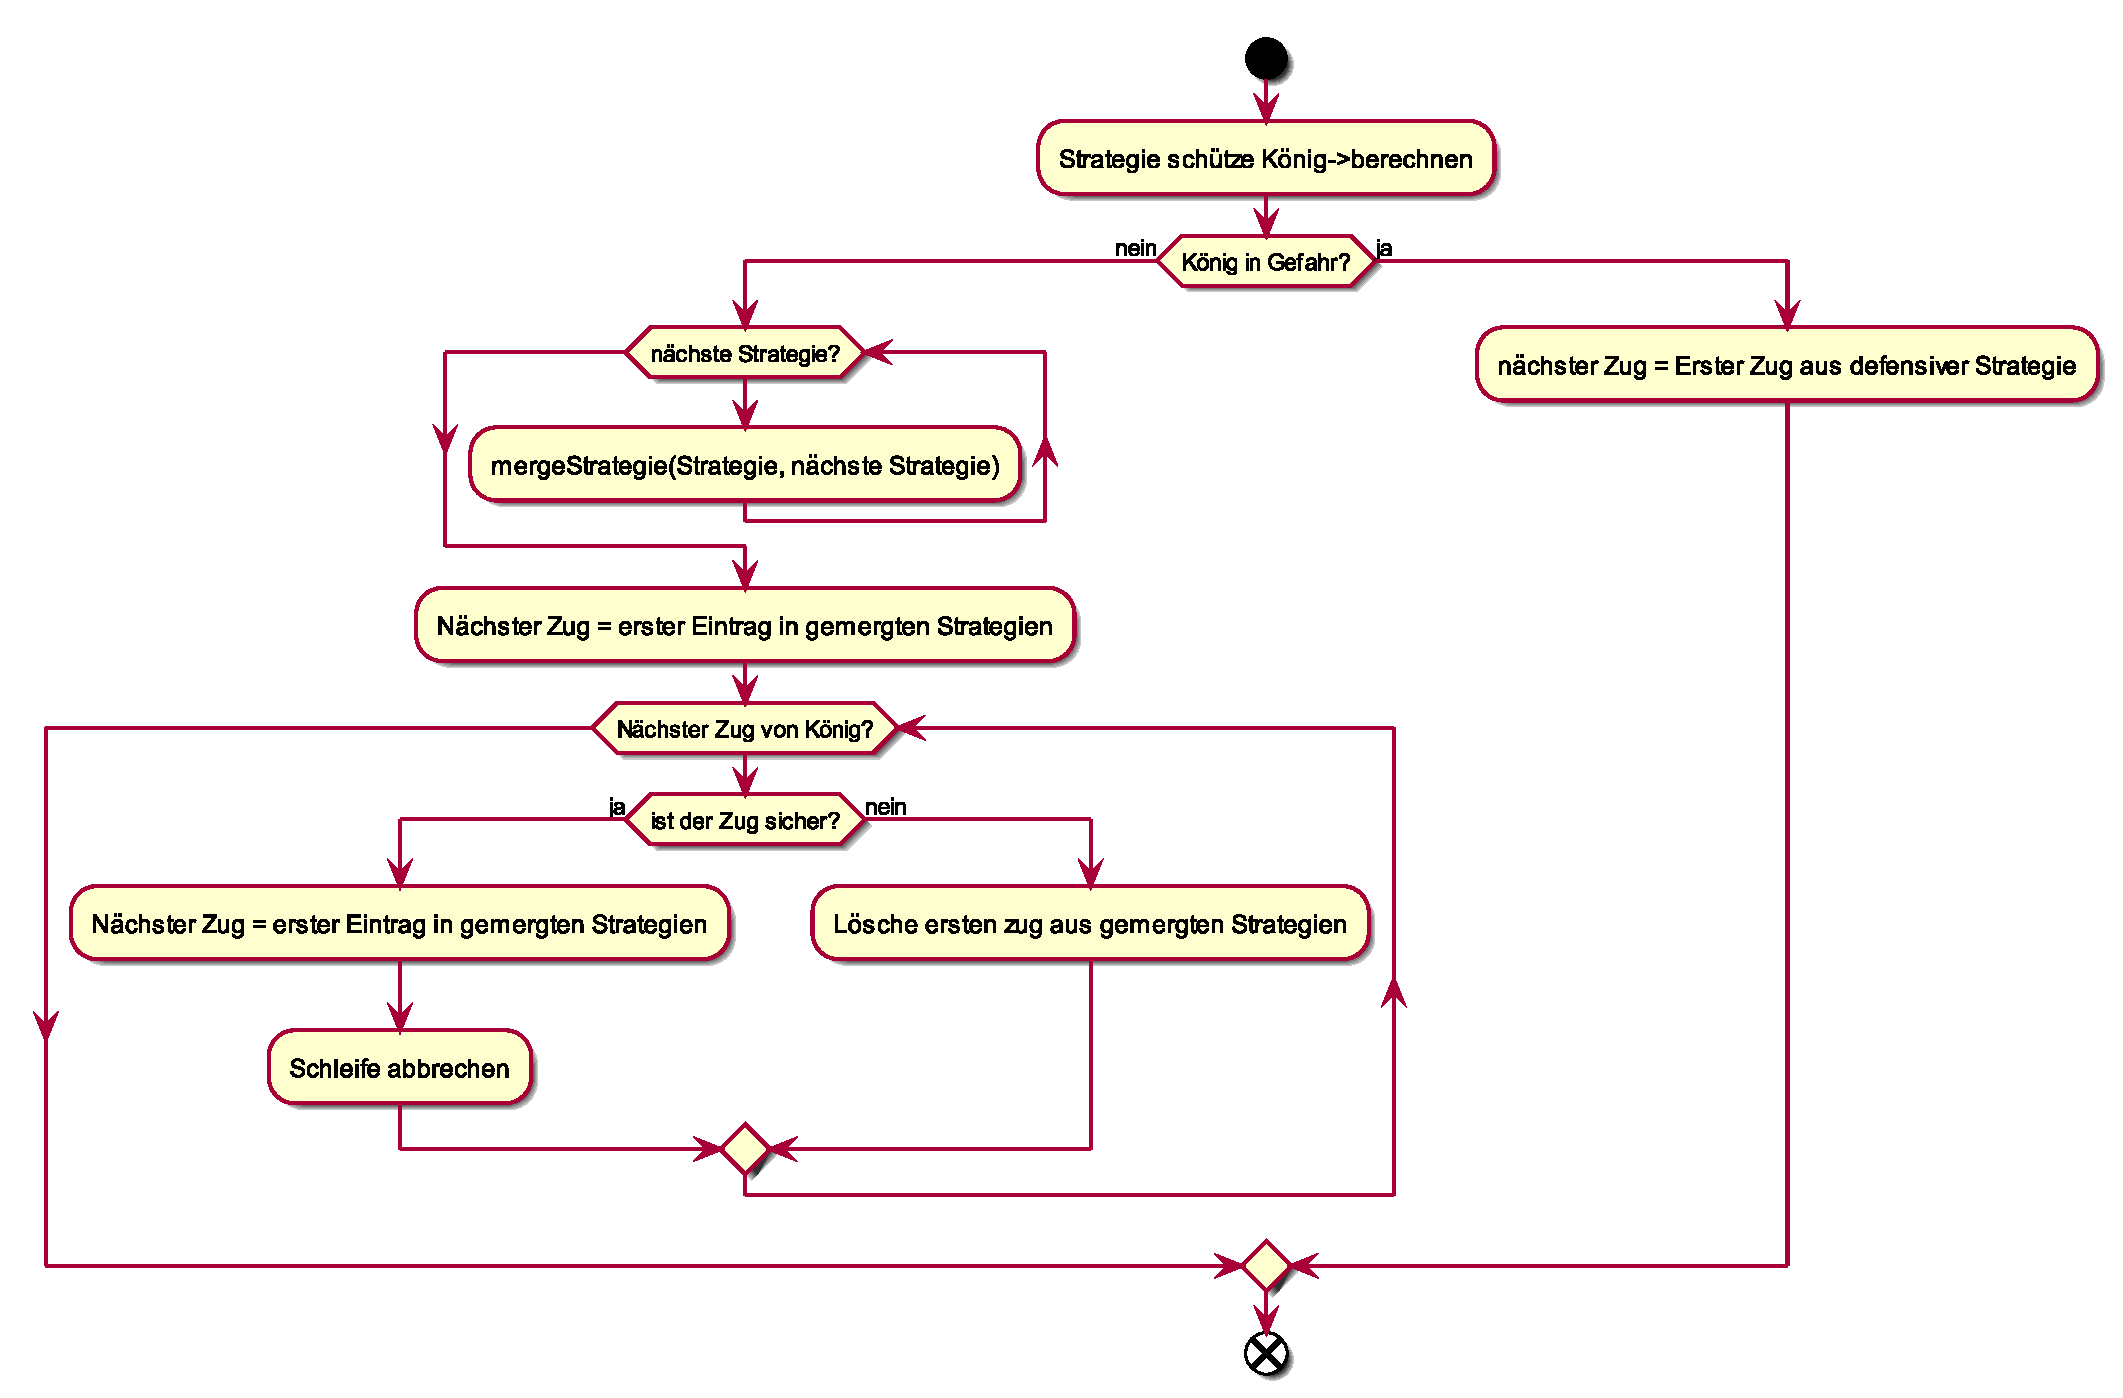
\includegraphics[width=\textwidth,height=\textheight/2,keepaspectratio=true]{KI_searchBestZug}}
\end{DoxyImageNoCaption}
  

Hier ist ein Graph, der zeigt, was diese Funktion aufruft\+:\nopagebreak
\begin{figure}[H]
\begin{center}
\leavevmode
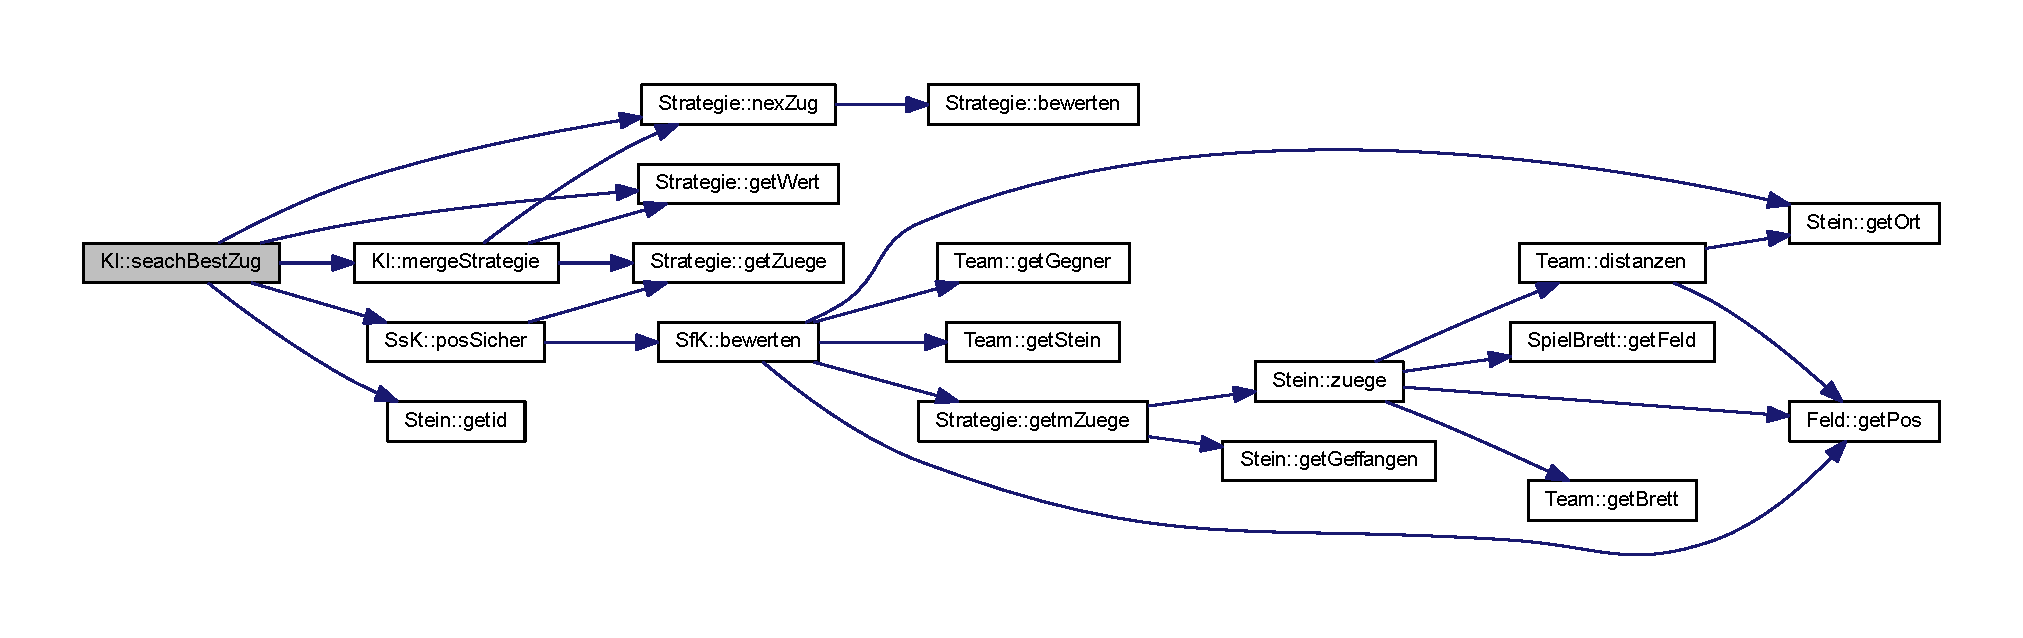
\includegraphics[width=350pt]{class_k_i_afa90fdb068e7b06e58db40b1ceeb8216_cgraph}
\end{center}
\end{figure}




\subsection{Dokumentation der Datenelemente}
\hypertarget{class_k_i_a93f7368fa6746ddb1e51d804ddaea096}{}\index{K\+I@{K\+I}!abrett@{abrett}}
\index{abrett@{abrett}!K\+I@{K\+I}}
\subsubsection[{abrett}]{\setlength{\rightskip}{0pt plus 5cm}{\bf Spiel\+Brett}\& K\+I\+::abrett\hspace{0.3cm}{\ttfamily [private]}}\label{class_k_i_a93f7368fa6746ddb1e51d804ddaea096}
\hypertarget{class_k_i_a16d7b067120b9b638781d5e5e6dcc005}{}\index{K\+I@{K\+I}!anzstrat@{anzstrat}}
\index{anzstrat@{anzstrat}!K\+I@{K\+I}}
\subsubsection[{anzstrat}]{\setlength{\rightskip}{0pt plus 5cm}const int K\+I\+::anzstrat =4\hspace{0.3cm}{\ttfamily [static]}, {\ttfamily [private]}}\label{class_k_i_a16d7b067120b9b638781d5e5e6dcc005}
\hypertarget{class_k_i_a34cb945060f752556a068ccf1771c531}{}\index{K\+I@{K\+I}!dv@{dv}}
\index{dv@{dv}!K\+I@{K\+I}}
\subsubsection[{dv}]{\setlength{\rightskip}{0pt plus 5cm}{\bf Ss\+K}$\ast$ K\+I\+::dv\hspace{0.3cm}{\ttfamily [private]}}\label{class_k_i_a34cb945060f752556a068ccf1771c531}
\hypertarget{class_k_i_acfefb24fdddb36cbfe2dff9e1d5d8296}{}\index{K\+I@{K\+I}!n\+Zug@{n\+Zug}}
\index{n\+Zug@{n\+Zug}!K\+I@{K\+I}}
\subsubsection[{n\+Zug}]{\setlength{\rightskip}{0pt plus 5cm}{\bf zug} K\+I\+::n\+Zug\hspace{0.3cm}{\ttfamily [private]}}\label{class_k_i_acfefb24fdddb36cbfe2dff9e1d5d8296}
\hypertarget{class_k_i_a6e07007b67f0a2778de3148ed5612921}{}\index{K\+I@{K\+I}!strat@{strat}}
\index{strat@{strat}!K\+I@{K\+I}}
\subsubsection[{strat}]{\setlength{\rightskip}{0pt plus 5cm}{\bf Strategie}$\ast$ K\+I\+::strat\mbox{[}{\bf anzstrat}\mbox{]}\hspace{0.3cm}{\ttfamily [private]}}\label{class_k_i_a6e07007b67f0a2778de3148ed5612921}
\hypertarget{class_k_i_a611b37548d94d9dce7e68024aa943733}{}\index{K\+I@{K\+I}!t@{t}}
\index{t@{t}!K\+I@{K\+I}}
\subsubsection[{t}]{\setlength{\rightskip}{0pt plus 5cm}{\bf Team}\& K\+I\+::t\hspace{0.3cm}{\ttfamily [private]}}\label{class_k_i_a611b37548d94d9dce7e68024aa943733}


Die Dokumentation für diese Klasse wurde erzeugt aufgrund der Dateien\+:\begin{DoxyCompactItemize}
\item 
\hyperlink{_k_i_8h}{K\+I.\+h}\item 
\hyperlink{_k_i_8cpp}{K\+I.\+cpp}\end{DoxyCompactItemize}

\hypertarget{class_koenig}{}\section{Koenig Klassenreferenz}
\label{class_koenig}\index{Koenig@{Koenig}}


{\ttfamily \#include $<$Koenig.\+h$>$}



Klassendiagramm für Koenig\+:\nopagebreak
\begin{figure}[H]
\begin{center}
\leavevmode
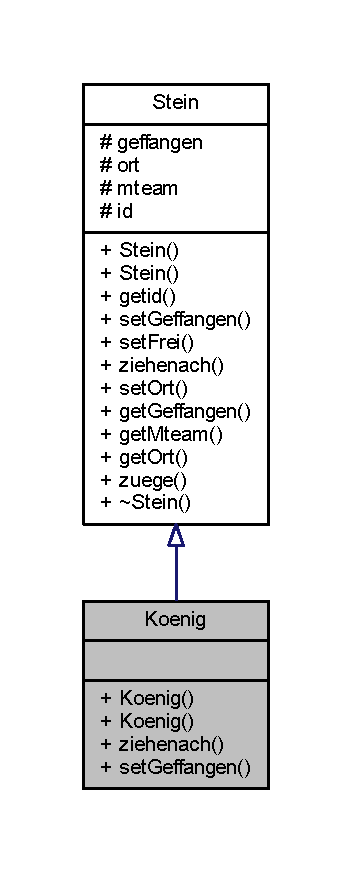
\includegraphics[width=169pt]{class_koenig__inherit__graph}
\end{center}
\end{figure}


Zusammengehörigkeiten von Koenig\+:\nopagebreak
\begin{figure}[H]
\begin{center}
\leavevmode
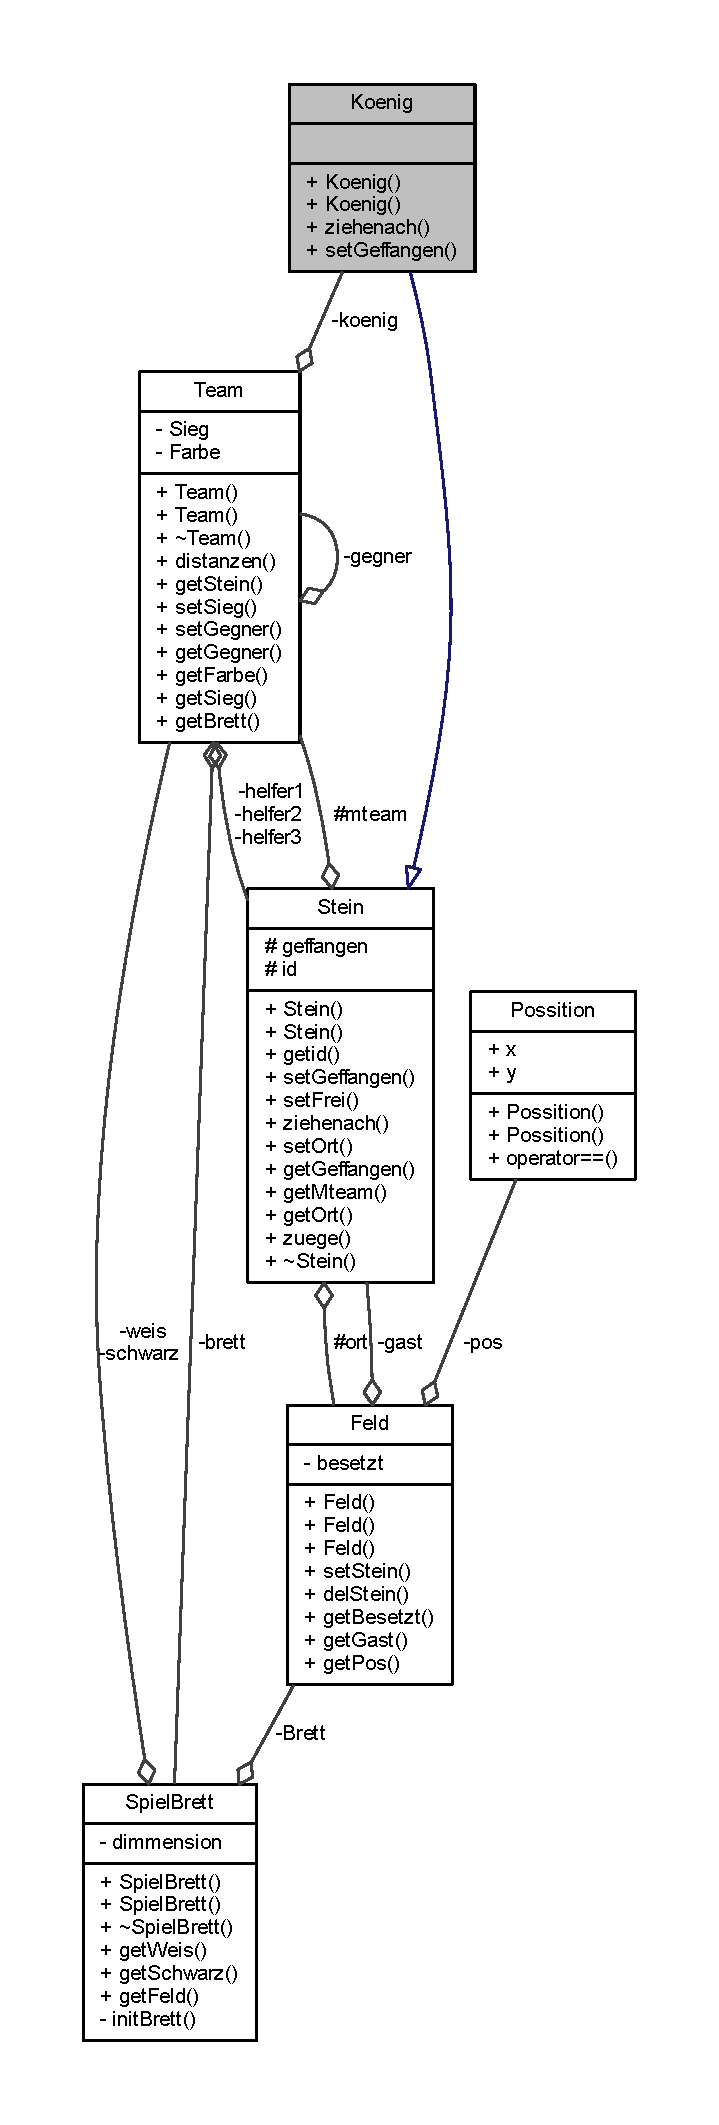
\includegraphics[height=550pt]{class_koenig__coll__graph}
\end{center}
\end{figure}
\subsection*{Öffentliche Methoden}
\begin{DoxyCompactItemize}
\item 
\hyperlink{class_koenig_a213d4b6961d0709bd1b48e469c7e5edf}{Koenig} ()
\item 
\hyperlink{class_koenig_a66858d9341213d157c1e478b74efb974}{Koenig} (int \hyperlink{class_stein_ab8a179db9a227d710ce7d236ecae37ee}{id}, \hyperlink{class_feld}{Feld} $\ast$startplatz, \hyperlink{class_team}{Team} $\ast$mt)
\item 
virtual bool \hyperlink{class_koenig_a6060e36b885b96aad97fa4c66646942f}{ziehenach} (\hyperlink{class_feld}{Feld} $\ast$ziehe) override
\item 
virtual void \hyperlink{class_koenig_a66d3242a51e934cc35bb8adabdba8a4a}{set\+Geffangen} () override
\end{DoxyCompactItemize}
\subsection*{Weitere Geerbte Elemente}


\subsection{Beschreibung der Konstruktoren und Destruktoren}
\hypertarget{class_koenig_a213d4b6961d0709bd1b48e469c7e5edf}{}\index{Koenig@{Koenig}!Koenig@{Koenig}}
\index{Koenig@{Koenig}!Koenig@{Koenig}}
\subsubsection[{Koenig}]{\setlength{\rightskip}{0pt plus 5cm}Koenig\+::\+Koenig (
\begin{DoxyParamCaption}
{}
\end{DoxyParamCaption}
)}\label{class_koenig_a213d4b6961d0709bd1b48e469c7e5edf}
\hypertarget{class_koenig_a66858d9341213d157c1e478b74efb974}{}\index{Koenig@{Koenig}!Koenig@{Koenig}}
\index{Koenig@{Koenig}!Koenig@{Koenig}}
\subsubsection[{Koenig}]{\setlength{\rightskip}{0pt plus 5cm}Koenig\+::\+Koenig (
\begin{DoxyParamCaption}
\item[{int}]{id, }
\item[{{\bf Feld} $\ast$}]{startplatz, }
\item[{{\bf Team} $\ast$}]{mt}
\end{DoxyParamCaption}
)}\label{class_koenig_a66858d9341213d157c1e478b74efb974}


\subsection{Dokumentation der Elementfunktionen}
\hypertarget{class_koenig_a66d3242a51e934cc35bb8adabdba8a4a}{}\index{Koenig@{Koenig}!set\+Geffangen@{set\+Geffangen}}
\index{set\+Geffangen@{set\+Geffangen}!Koenig@{Koenig}}
\subsubsection[{set\+Geffangen}]{\setlength{\rightskip}{0pt plus 5cm}void Koenig\+::set\+Geffangen (
\begin{DoxyParamCaption}
{}
\end{DoxyParamCaption}
)\hspace{0.3cm}{\ttfamily [override]}, {\ttfamily [virtual]}}\label{class_koenig_a66d3242a51e934cc35bb8adabdba8a4a}
ziehenach(\+Feld) Mit dieser Methode hat der König die Möglichkeit seine Helfer zu befreien und sich auf dem Spielfeld zu bewegen.


\begin{DoxyParams}{Parameter}
{\em \mbox{[}\+Feld\mbox{]}} & $\ast$ziehe hierbei handelt sich um einen Pointer auf das \hyperlink{class_feld}{Feld}, das er springen soll\\
\hline
\end{DoxyParams}
  

Erneute Implementation von \hyperlink{class_stein_a8a98cf8c96426bf5164c6eb41b03154b}{Stein}.



Hier ist ein Graph, der zeigt, was diese Funktion aufruft\+:\nopagebreak
\begin{figure}[H]
\begin{center}
\leavevmode
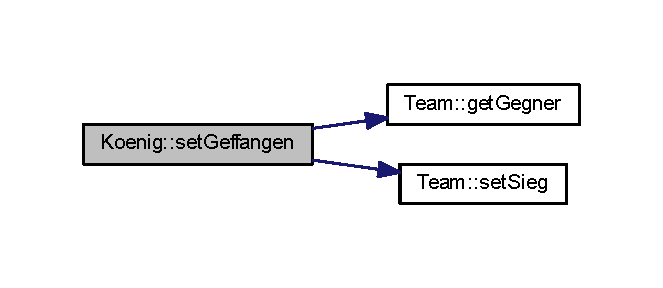
\includegraphics[width=318pt]{class_koenig_a66d3242a51e934cc35bb8adabdba8a4a_cgraph}
\end{center}
\end{figure}


\hypertarget{class_koenig_a6060e36b885b96aad97fa4c66646942f}{}\index{Koenig@{Koenig}!ziehenach@{ziehenach}}
\index{ziehenach@{ziehenach}!Koenig@{Koenig}}
\subsubsection[{ziehenach}]{\setlength{\rightskip}{0pt plus 5cm}bool Koenig\+::ziehenach (
\begin{DoxyParamCaption}
\item[{{\bf Feld} $\ast$}]{ziehe}
\end{DoxyParamCaption}
)\hspace{0.3cm}{\ttfamily [override]}, {\ttfamily [virtual]}}\label{class_koenig_a6060e36b885b96aad97fa4c66646942f}
Implementiert den Startplatz des Königs. 

Erneute Implementation von \hyperlink{class_stein_afdac18155661536e25eda360038c1ca7}{Stein}.



Hier ist ein Graph, der zeigt, was diese Funktion aufruft\+:\nopagebreak
\begin{figure}[H]
\begin{center}
\leavevmode
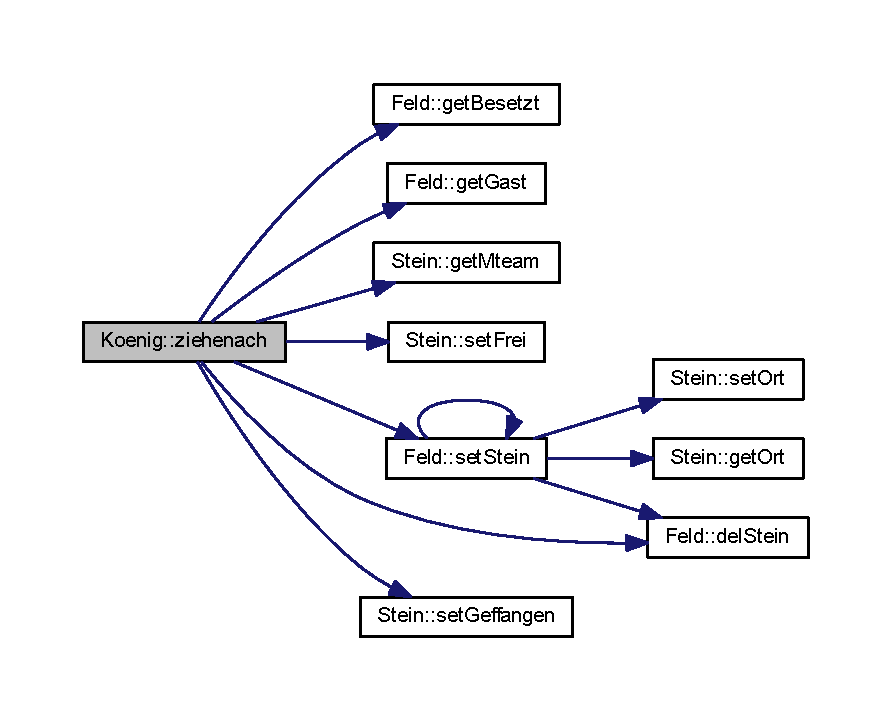
\includegraphics[width=350pt]{class_koenig_a6060e36b885b96aad97fa4c66646942f_cgraph}
\end{center}
\end{figure}




Die Dokumentation für diese Klasse wurde erzeugt aufgrund der Dateien\+:\begin{DoxyCompactItemize}
\item 
\hyperlink{_koenig_8h}{Koenig.\+h}\item 
\hyperlink{_koenig_8cpp}{Koenig.\+cpp}\end{DoxyCompactItemize}

\hypertarget{struct_possition}{}\section{Possition Strukturreferenz}
\label{struct_possition}\index{Possition@{Possition}}


{\ttfamily \#include $<$Possition.\+h$>$}



Zusammengehörigkeiten von Possition\+:\nopagebreak
\begin{figure}[H]
\begin{center}
\leavevmode
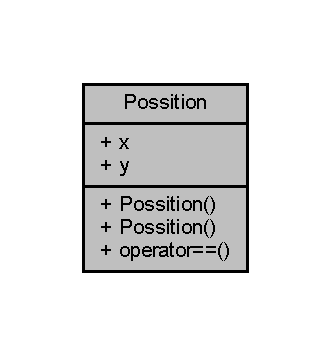
\includegraphics[width=159pt]{struct_possition__coll__graph}
\end{center}
\end{figure}
\subsection*{Öffentliche Methoden}
\begin{DoxyCompactItemize}
\item 
\hyperlink{struct_possition_aeca027993a6ef360904208411c5e7708}{Possition} (short int \hyperlink{struct_possition_a07b558914470911fd3c10a745b0c7bc2}{x}, short int \hyperlink{struct_possition_ad3af285b52a6199147abcd48ebf83624}{y})
\item 
\hyperlink{struct_possition_a23d4588228d627c48b7b2c5209271b0d}{Possition} ()
\item 
bool \hyperlink{struct_possition_a53040dcec3906f26210fc328230cc4c4}{operator==} (const \hyperlink{struct_possition}{Possition} \&p) const 
\end{DoxyCompactItemize}
\subsection*{Öffentliche Attribute}
\begin{DoxyCompactItemize}
\item 
short int \hyperlink{struct_possition_a07b558914470911fd3c10a745b0c7bc2}{x}
\item 
short int \hyperlink{struct_possition_ad3af285b52a6199147abcd48ebf83624}{y}
\end{DoxyCompactItemize}


\subsection{Ausführliche Beschreibung}
struct Position 

\subsection{Beschreibung der Konstruktoren und Destruktoren}
\hypertarget{struct_possition_aeca027993a6ef360904208411c5e7708}{}\index{Possition@{Possition}!Possition@{Possition}}
\index{Possition@{Possition}!Possition@{Possition}}
\subsubsection[{Possition}]{\setlength{\rightskip}{0pt plus 5cm}Possition\+::\+Possition (
\begin{DoxyParamCaption}
\item[{short int}]{x, }
\item[{short int}]{y}
\end{DoxyParamCaption}
)\hspace{0.3cm}{\ttfamily [inline]}}\label{struct_possition_aeca027993a6ef360904208411c5e7708}
\hypertarget{struct_possition_a23d4588228d627c48b7b2c5209271b0d}{}\index{Possition@{Possition}!Possition@{Possition}}
\index{Possition@{Possition}!Possition@{Possition}}
\subsubsection[{Possition}]{\setlength{\rightskip}{0pt plus 5cm}Possition\+::\+Possition (
\begin{DoxyParamCaption}
{}
\end{DoxyParamCaption}
)\hspace{0.3cm}{\ttfamily [inline]}}\label{struct_possition_a23d4588228d627c48b7b2c5209271b0d}


\subsection{Dokumentation der Elementfunktionen}
\hypertarget{struct_possition_a53040dcec3906f26210fc328230cc4c4}{}\index{Possition@{Possition}!operator==@{operator==}}
\index{operator==@{operator==}!Possition@{Possition}}
\subsubsection[{operator==}]{\setlength{\rightskip}{0pt plus 5cm}bool Possition\+::operator== (
\begin{DoxyParamCaption}
\item[{const {\bf Possition} \&}]{p}
\end{DoxyParamCaption}
) const\hspace{0.3cm}{\ttfamily [inline]}}\label{struct_possition_a53040dcec3906f26210fc328230cc4c4}


\subsection{Dokumentation der Datenelemente}
\hypertarget{struct_possition_a07b558914470911fd3c10a745b0c7bc2}{}\index{Possition@{Possition}!x@{x}}
\index{x@{x}!Possition@{Possition}}
\subsubsection[{x}]{\setlength{\rightskip}{0pt plus 5cm}short int Possition\+::x}\label{struct_possition_a07b558914470911fd3c10a745b0c7bc2}
\hypertarget{struct_possition_ad3af285b52a6199147abcd48ebf83624}{}\index{Possition@{Possition}!y@{y}}
\index{y@{y}!Possition@{Possition}}
\subsubsection[{y}]{\setlength{\rightskip}{0pt plus 5cm}short int Possition\+::y}\label{struct_possition_ad3af285b52a6199147abcd48ebf83624}


Die Dokumentation für diese Struktur wurde erzeugt aufgrund der Datei\+:\begin{DoxyCompactItemize}
\item 
\hyperlink{_possition_8h}{Possition.\+h}\end{DoxyCompactItemize}

\hypertarget{class_sf_h}{}\section{Sf\+H Klassenreferenz}
\label{class_sf_h}\index{Sf\+H@{Sf\+H}}


{\ttfamily \#include $<$Sf\+H.\+h$>$}



Klassendiagramm für Sf\+H\+:\nopagebreak
\begin{figure}[H]
\begin{center}
\leavevmode
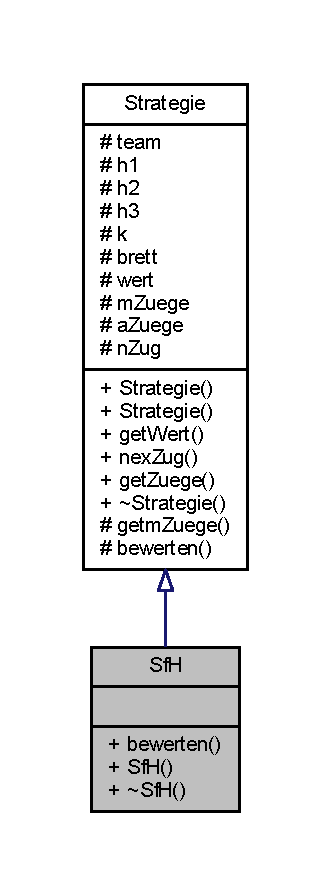
\includegraphics[width=159pt]{class_sf_h__inherit__graph}
\end{center}
\end{figure}


Zusammengehörigkeiten von Sf\+H\+:\nopagebreak
\begin{figure}[H]
\begin{center}
\leavevmode
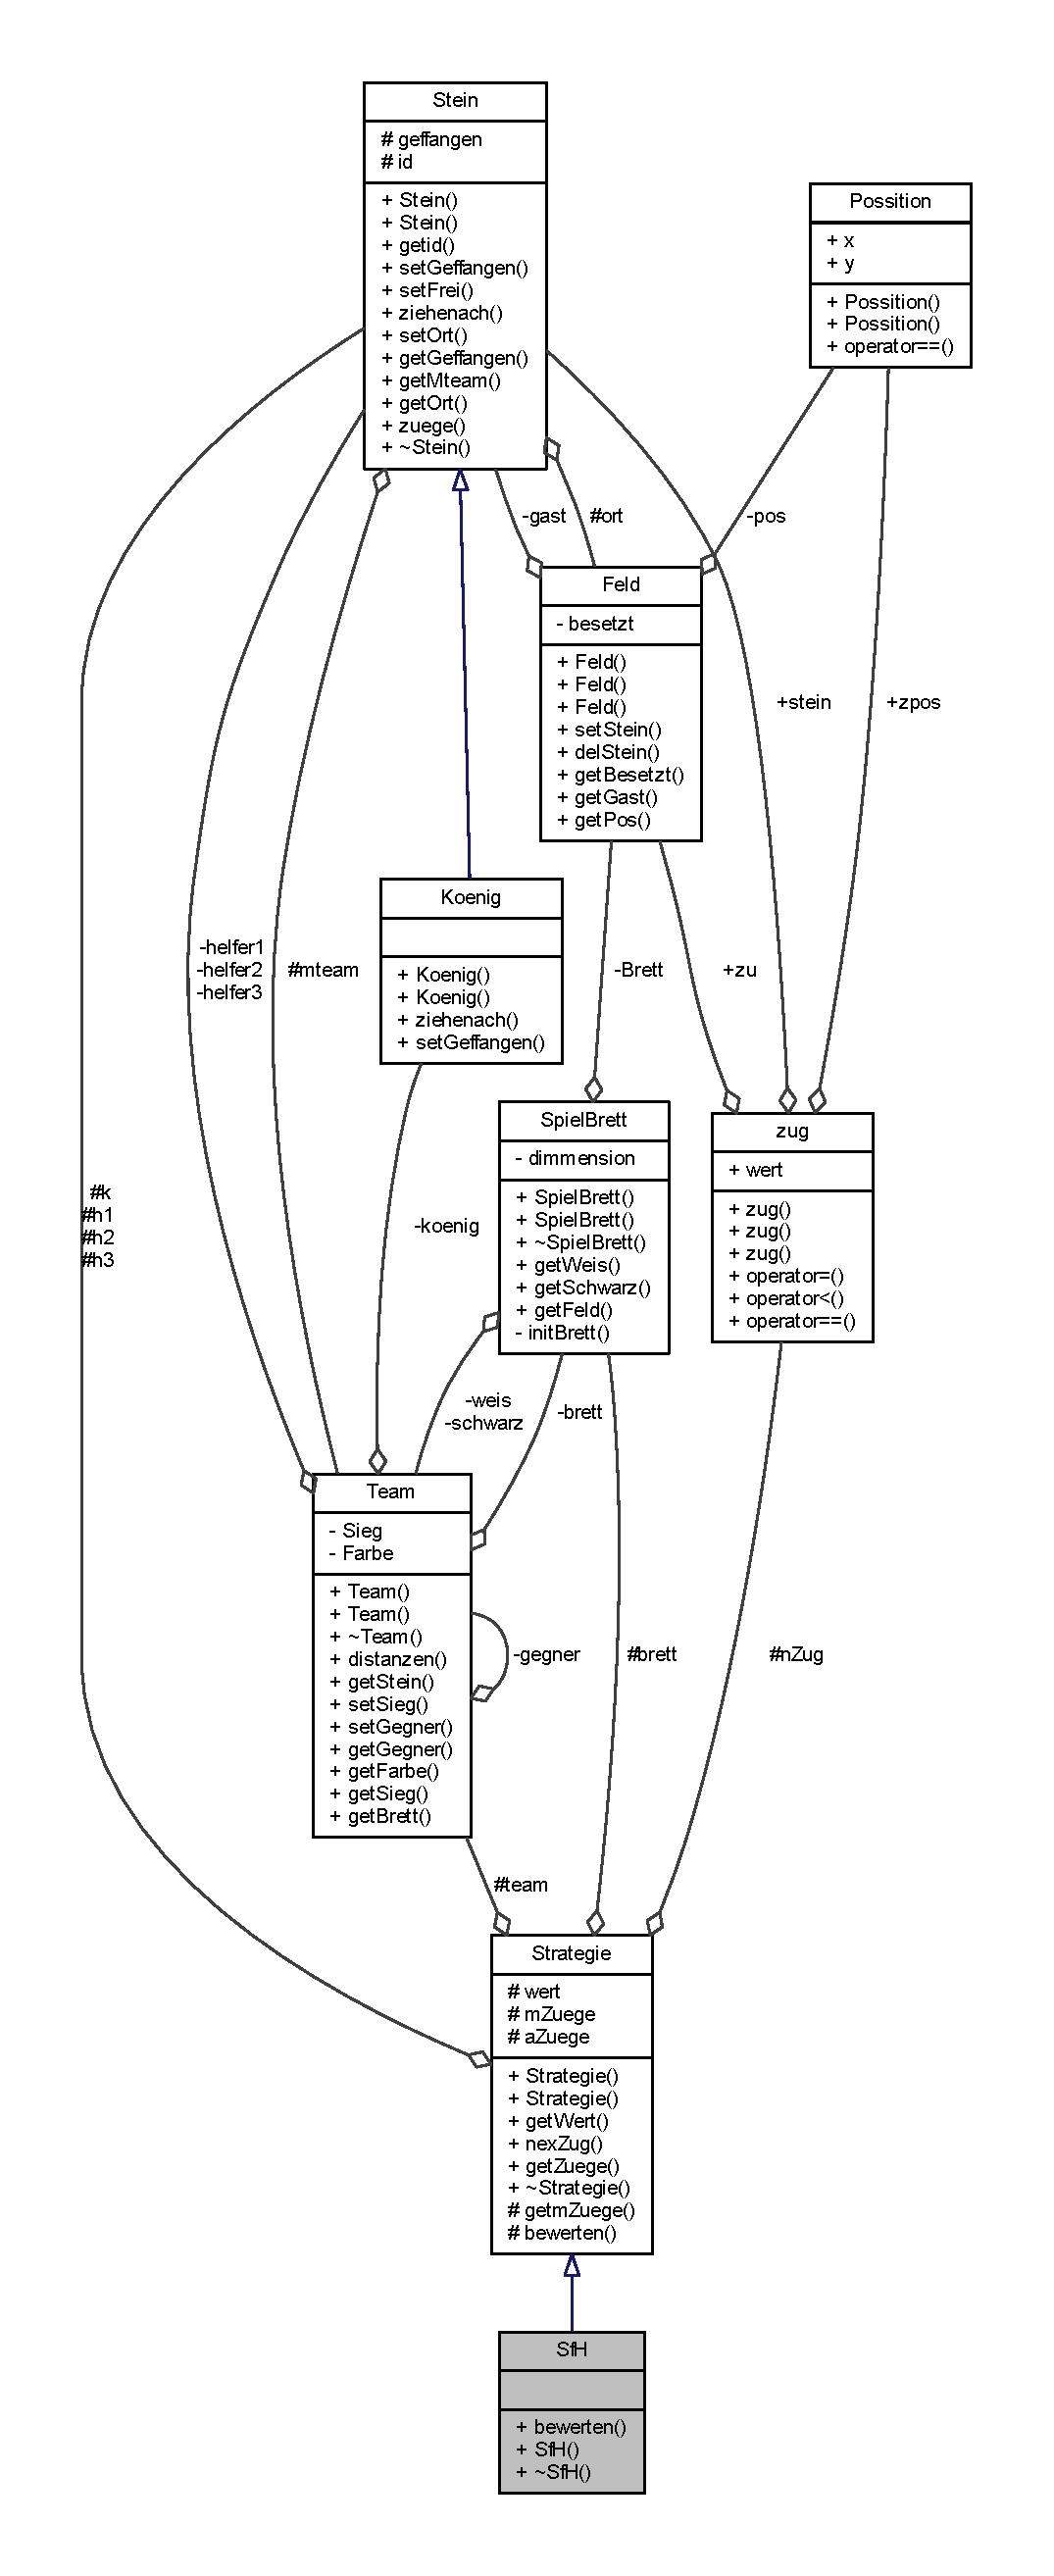
\includegraphics[height=550pt]{class_sf_h__coll__graph}
\end{center}
\end{figure}
\subsection*{Öffentliche Methoden}
\begin{DoxyCompactItemize}
\item 
virtual void \hyperlink{class_sf_h_a9790a3fab6619e16961568d735678d4f}{bewerten} () override
\item 
\hyperlink{class_sf_h_a97daf9dffa4529ca2ed4ce98ac9d0e67}{Sf\+H} (\hyperlink{class_team}{Team} \&\hyperlink{class_strategie_a4f55e74f189ec8c6df88a57119fb3def}{team}, \hyperlink{class_spiel_brett}{Spiel\+Brett} \&b)
\item 
virtual \hyperlink{class_sf_h_a320c8f54cfd3a4ab7759a4c76cf08877}{$\sim$\+Sf\+H} ()
\end{DoxyCompactItemize}
\subsection*{Weitere Geerbte Elemente}


\subsection{Ausführliche Beschreibung}
class \hyperlink{class_sf_h}{Sf\+H} (\hyperlink{class_strategie}{Strategie} fange Helfer) implementiert die Methode \hyperlink{class_sf_h_a9790a3fab6619e16961568d735678d4f}{bewerten()}; \subparagraph*{}

Diese \hyperlink{class_strategie}{Strategie} sorgt dafür, dass die gegnerischen Helfer festgesetzt/gefangen werden. Ein festgesetzter/gefangener Helfer stellt insofern keine Bedrohung mehr dar, bis er wieder vom \hyperlink{class_koenig}{Koenig} befreit wird. Dies gilt es durch andere Strategien zu verhindern. \subparagraph*{}


\begin{DoxyParams}{Parameter}
{\em \&team} & Referenz auf Instanz von \hyperlink{class_team}{Team} \\
\hline
{\em \&b} & Referenz auf Instanz von \hyperlink{class_spiel_brett}{Spiel\+Brett} \\
\hline
\end{DoxyParams}


\subsection{Beschreibung der Konstruktoren und Destruktoren}
\hypertarget{class_sf_h_a97daf9dffa4529ca2ed4ce98ac9d0e67}{}\index{Sf\+H@{Sf\+H}!Sf\+H@{Sf\+H}}
\index{Sf\+H@{Sf\+H}!Sf\+H@{Sf\+H}}
\subsubsection[{Sf\+H}]{\setlength{\rightskip}{0pt plus 5cm}Sf\+H\+::\+Sf\+H (
\begin{DoxyParamCaption}
\item[{{\bf Team} \&}]{team, }
\item[{{\bf Spiel\+Brett} \&}]{b}
\end{DoxyParamCaption}
)}\label{class_sf_h_a97daf9dffa4529ca2ed4ce98ac9d0e67}
\hypertarget{class_sf_h_a320c8f54cfd3a4ab7759a4c76cf08877}{}\index{Sf\+H@{Sf\+H}!````~Sf\+H@{$\sim$\+Sf\+H}}
\index{````~Sf\+H@{$\sim$\+Sf\+H}!Sf\+H@{Sf\+H}}
\subsubsection[{$\sim$\+Sf\+H}]{\setlength{\rightskip}{0pt plus 5cm}Sf\+H\+::$\sim$\+Sf\+H (
\begin{DoxyParamCaption}
{}
\end{DoxyParamCaption}
)\hspace{0.3cm}{\ttfamily [virtual]}}\label{class_sf_h_a320c8f54cfd3a4ab7759a4c76cf08877}


\subsection{Dokumentation der Elementfunktionen}
\hypertarget{class_sf_h_a9790a3fab6619e16961568d735678d4f}{}\index{Sf\+H@{Sf\+H}!bewerten@{bewerten}}
\index{bewerten@{bewerten}!Sf\+H@{Sf\+H}}
\subsubsection[{bewerten}]{\setlength{\rightskip}{0pt plus 5cm}void Sf\+H\+::bewerten (
\begin{DoxyParamCaption}
{}
\end{DoxyParamCaption}
)\hspace{0.3cm}{\ttfamily [override]}, {\ttfamily [virtual]}}\label{class_sf_h_a9790a3fab6619e16961568d735678d4f}
\hyperlink{class_sf_h_a9790a3fab6619e16961568d735678d4f}{bewerten()} Bewertet mögliche Züge nach der Möglichkeit gegnerische Helfer zu fangen.  
\begin{DoxyImageNoCaption}
  \mbox{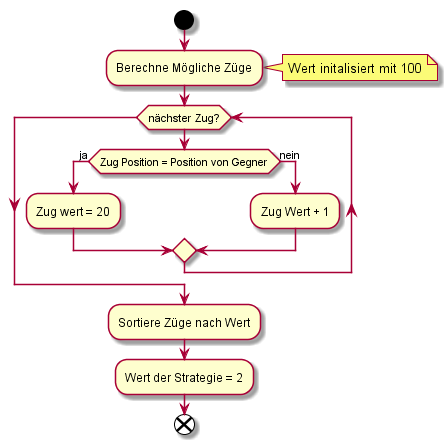
\includegraphics[width=\textwidth,height=\textheight/2,keepaspectratio=true]{SfH_bewerten.png}}
\end{DoxyImageNoCaption}
  

Implementiert \hyperlink{class_strategie_a6e11413c1c8e4ca8bd0bcac21be3c1bf}{Strategie}.



Hier ist ein Graph, der zeigt, was diese Funktion aufruft\+:\nopagebreak
\begin{figure}[H]
\begin{center}
\leavevmode
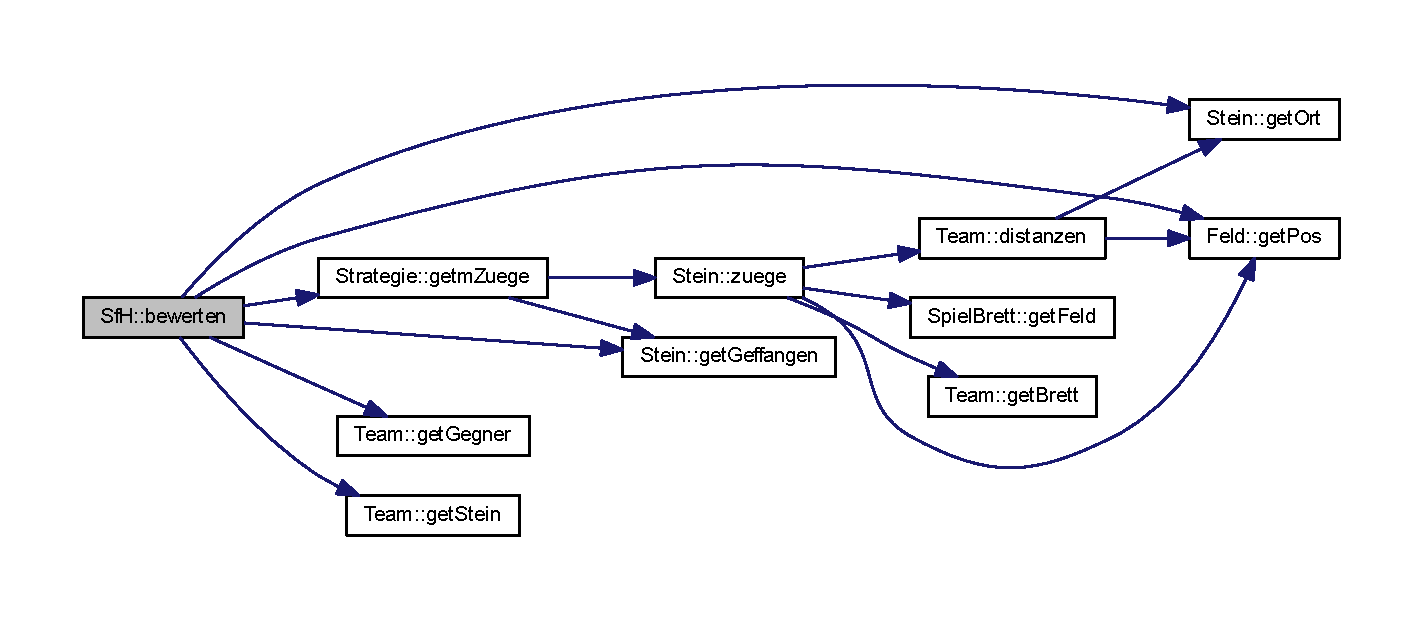
\includegraphics[width=350pt]{class_sf_h_a9790a3fab6619e16961568d735678d4f_cgraph}
\end{center}
\end{figure}




Die Dokumentation für diese Klasse wurde erzeugt aufgrund der Dateien\+:\begin{DoxyCompactItemize}
\item 
\hyperlink{_sf_h_8h}{Sf\+H.\+h}\item 
\hyperlink{_sf_h_8cpp}{Sf\+H.\+cpp}\end{DoxyCompactItemize}

\hypertarget{class_sf_k}{}\section{Sf\+K Klassenreferenz}
\label{class_sf_k}\index{Sf\+K@{Sf\+K}}


{\ttfamily \#include $<$Sf\+K.\+h$>$}



Klassendiagramm für Sf\+K\+:\nopagebreak
\begin{figure}[H]
\begin{center}
\leavevmode
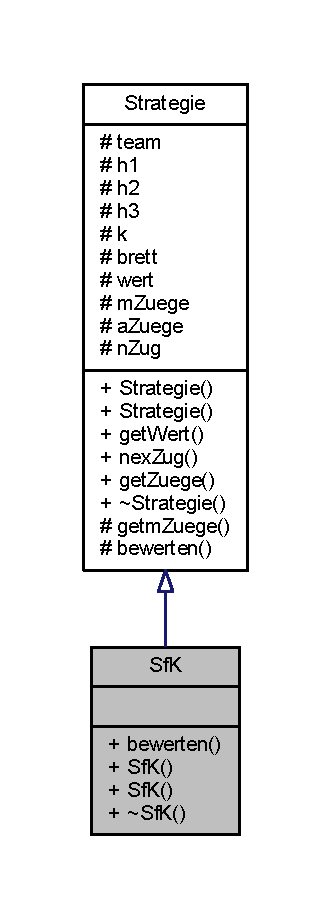
\includegraphics[width=159pt]{class_sf_k__inherit__graph}
\end{center}
\end{figure}


Zusammengehörigkeiten von Sf\+K\+:\nopagebreak
\begin{figure}[H]
\begin{center}
\leavevmode
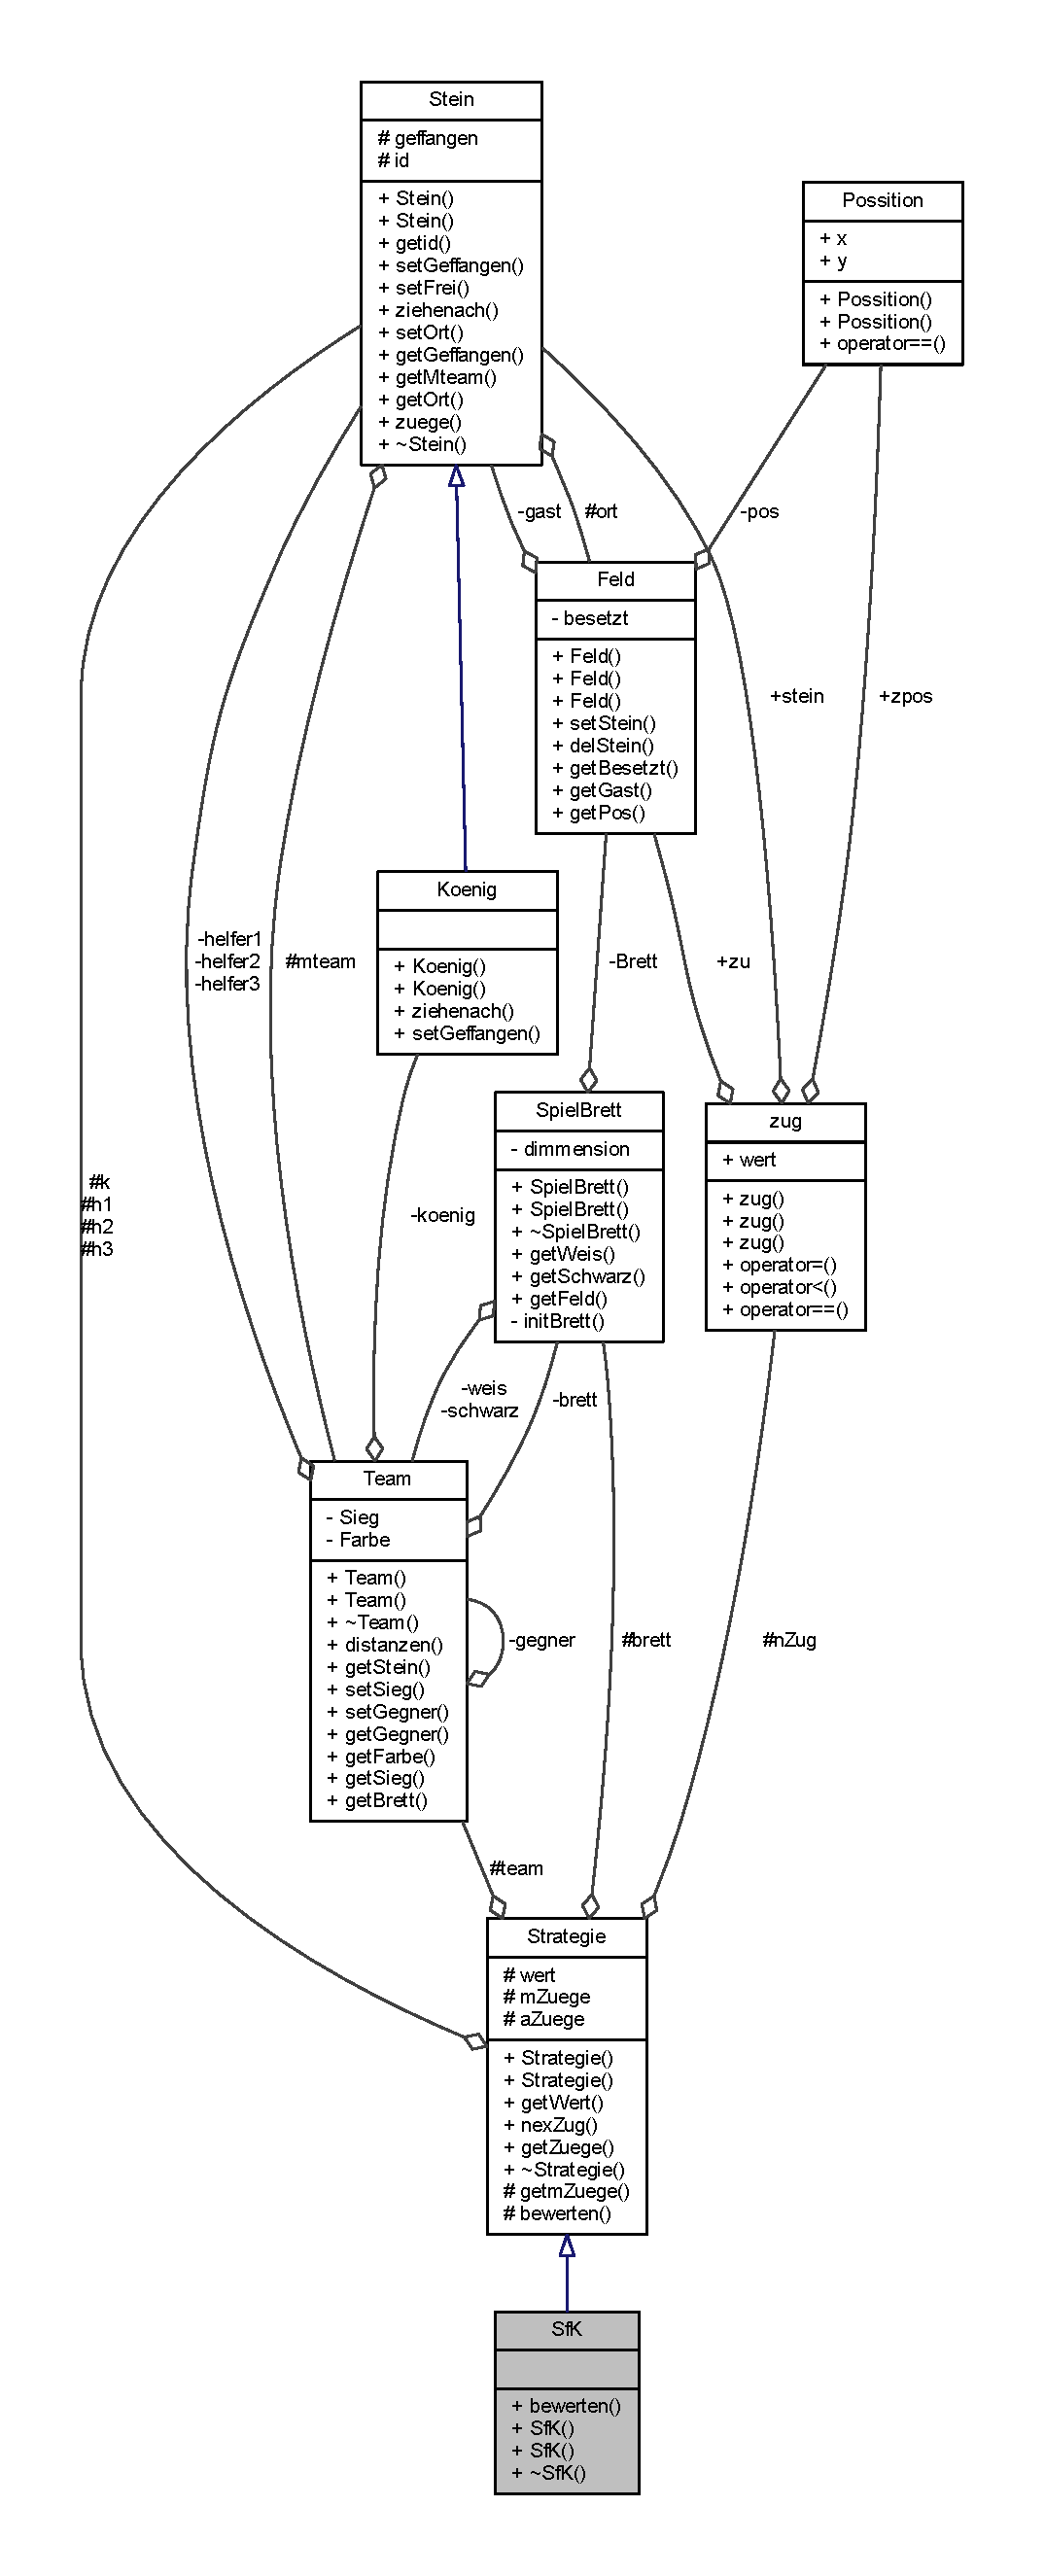
\includegraphics[height=550pt]{class_sf_k__coll__graph}
\end{center}
\end{figure}
\subsection*{Öffentliche Methoden}
\begin{DoxyCompactItemize}
\item 
virtual void \hyperlink{class_sf_k_a54410f0aa0c2f76704a0eb181a5737f0}{bewerten} () override
\item 
\hyperlink{class_sf_k_ae54f5f252db3e81aac89de1cdf4db5b2}{Sf\+K} (\hyperlink{class_team}{Team} \&\hyperlink{class_strategie_a4f55e74f189ec8c6df88a57119fb3def}{team}, \hyperlink{class_spiel_brett}{Spiel\+Brett} \&b)
\item 
\hyperlink{class_sf_k_a0b2852d8f0518f85092ec55db9ac3fd4}{Sf\+K} ()
\item 
virtual \hyperlink{class_sf_k_a5cd7cf22bfa7535a5a43a975595b73b7}{$\sim$\+Sf\+K} ()
\end{DoxyCompactItemize}
\subsection*{Weitere Geerbte Elemente}


\subsection{Ausführliche Beschreibung}
class \hyperlink{class_sf_k}{Sf\+K} (\hyperlink{class_strategie}{Strategie} fange König) Ist eine Ableitung der abstrakten Klasse \hyperlink{class_strategie}{Strategie}. \subparagraph*{}

Diese \hyperlink{class_strategie}{Strategie} sorgt dafür, dass sich die Spielfiguren dem gegnerischen König nähern, um in festsetzen/gefangen nehmen zu können. Ein festgesetzter/gefangener König bedeutet das Spielende. Ein Sieg wird erzielt, sobald der gegnerische König festgesetzt/gefangen ist. \subparagraph*{}

Überschreibt/implementiert die Methode \hyperlink{class_sf_k_a54410f0aa0c2f76704a0eb181a5737f0}{bewerten()}; 
\begin{DoxyParams}{Parameter}
{\em \&team} & Referenz auf Instanz von \hyperlink{class_team}{Team} \\
\hline
{\em \&b} & Referenz auf Instanz von \hyperlink{class_spiel_brett}{Spiel\+Brett} \\
\hline
\end{DoxyParams}


\subsection{Beschreibung der Konstruktoren und Destruktoren}
\hypertarget{class_sf_k_ae54f5f252db3e81aac89de1cdf4db5b2}{}\index{Sf\+K@{Sf\+K}!Sf\+K@{Sf\+K}}
\index{Sf\+K@{Sf\+K}!Sf\+K@{Sf\+K}}
\subsubsection[{Sf\+K}]{\setlength{\rightskip}{0pt plus 5cm}Sf\+K\+::\+Sf\+K (
\begin{DoxyParamCaption}
\item[{{\bf Team} \&}]{team, }
\item[{{\bf Spiel\+Brett} \&}]{b}
\end{DoxyParamCaption}
)}\label{class_sf_k_ae54f5f252db3e81aac89de1cdf4db5b2}
\hypertarget{class_sf_k_a0b2852d8f0518f85092ec55db9ac3fd4}{}\index{Sf\+K@{Sf\+K}!Sf\+K@{Sf\+K}}
\index{Sf\+K@{Sf\+K}!Sf\+K@{Sf\+K}}
\subsubsection[{Sf\+K}]{\setlength{\rightskip}{0pt plus 5cm}Sf\+K\+::\+Sf\+K (
\begin{DoxyParamCaption}
{}
\end{DoxyParamCaption}
)}\label{class_sf_k_a0b2852d8f0518f85092ec55db9ac3fd4}
\hypertarget{class_sf_k_a5cd7cf22bfa7535a5a43a975595b73b7}{}\index{Sf\+K@{Sf\+K}!````~Sf\+K@{$\sim$\+Sf\+K}}
\index{````~Sf\+K@{$\sim$\+Sf\+K}!Sf\+K@{Sf\+K}}
\subsubsection[{$\sim$\+Sf\+K}]{\setlength{\rightskip}{0pt plus 5cm}Sf\+K\+::$\sim$\+Sf\+K (
\begin{DoxyParamCaption}
{}
\end{DoxyParamCaption}
)\hspace{0.3cm}{\ttfamily [virtual]}}\label{class_sf_k_a5cd7cf22bfa7535a5a43a975595b73b7}


\subsection{Dokumentation der Elementfunktionen}
\hypertarget{class_sf_k_a54410f0aa0c2f76704a0eb181a5737f0}{}\index{Sf\+K@{Sf\+K}!bewerten@{bewerten}}
\index{bewerten@{bewerten}!Sf\+K@{Sf\+K}}
\subsubsection[{bewerten}]{\setlength{\rightskip}{0pt plus 5cm}void Sf\+K\+::bewerten (
\begin{DoxyParamCaption}
{}
\end{DoxyParamCaption}
)\hspace{0.3cm}{\ttfamily [override]}, {\ttfamily [virtual]}}\label{class_sf_k_a54410f0aa0c2f76704a0eb181a5737f0}
\hyperlink{class_sf_k_a54410f0aa0c2f76704a0eb181a5737f0}{bewerten()} Bewertet mögliche Züge nach der Möglichkeit gegnerischen König zu fangen.  
\begin{DoxyImageNoCaption}
  \mbox{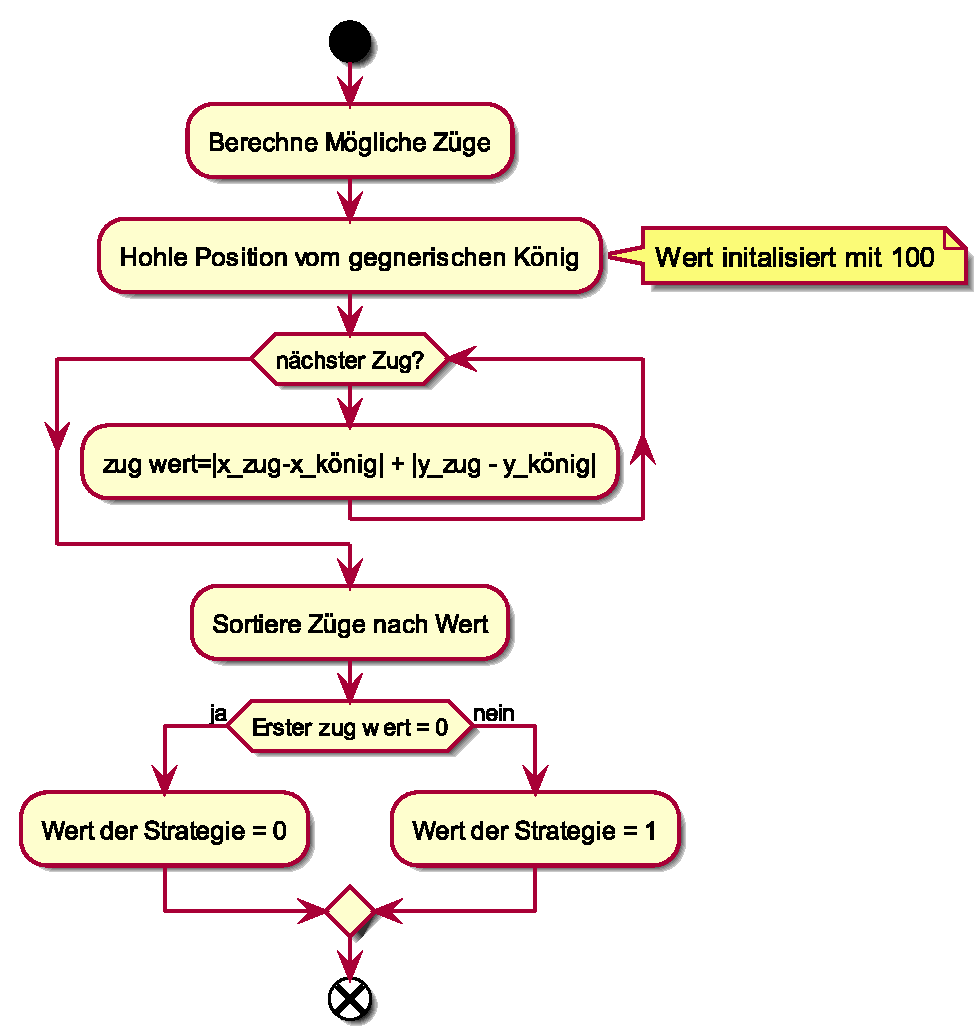
\includegraphics[width=\textwidth,height=\textheight/2,keepaspectratio=true]{SfK_bewerten}}
\end{DoxyImageNoCaption}
  

Implementiert \hyperlink{class_strategie_a6e11413c1c8e4ca8bd0bcac21be3c1bf}{Strategie}.



Hier ist ein Graph, der zeigt, was diese Funktion aufruft\+:\nopagebreak
\begin{figure}[H]
\begin{center}
\leavevmode
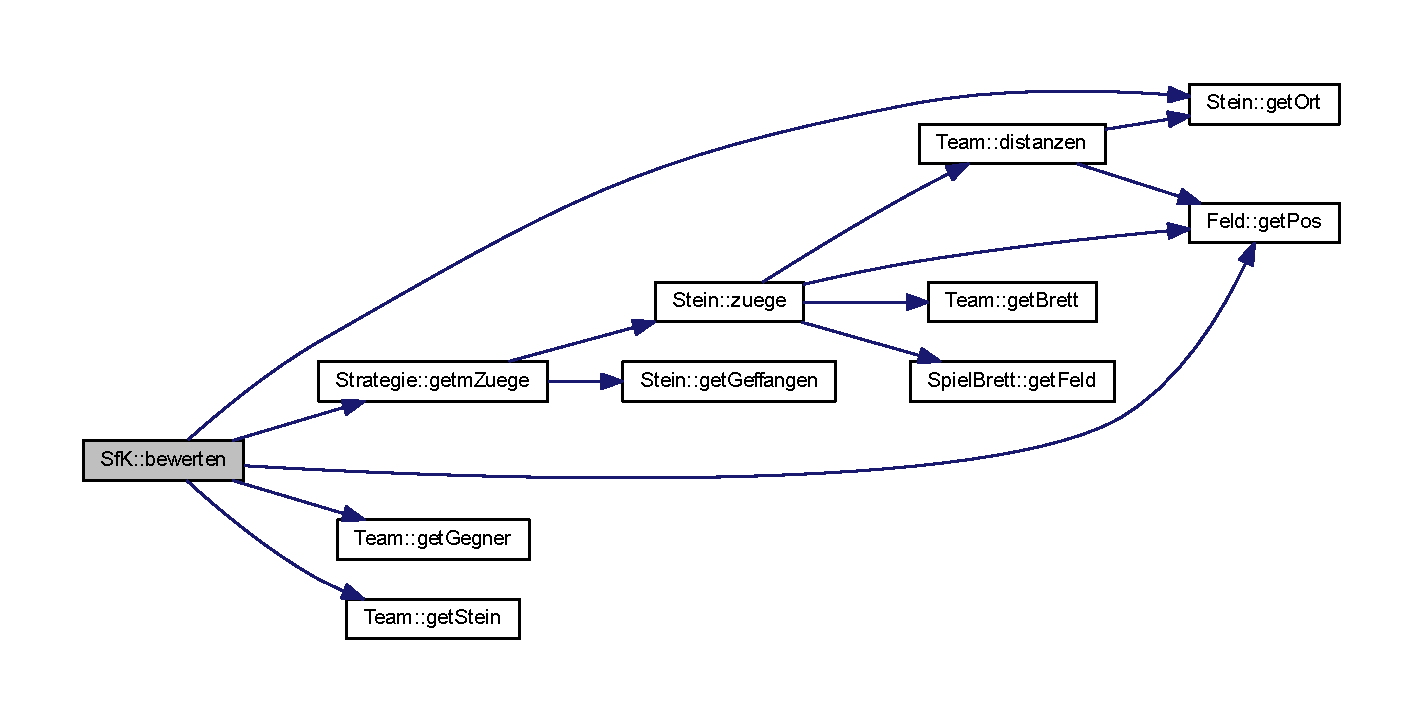
\includegraphics[width=350pt]{class_sf_k_a54410f0aa0c2f76704a0eb181a5737f0_cgraph}
\end{center}
\end{figure}




Die Dokumentation für diese Klasse wurde erzeugt aufgrund der Dateien\+:\begin{DoxyCompactItemize}
\item 
\hyperlink{_sf_k_8h}{Sf\+K.\+h}\item 
\hyperlink{_sf_k_8cpp}{Sf\+K.\+cpp}\end{DoxyCompactItemize}

\hypertarget{class_spiel_brett}{}\section{Spiel\+Brett Klassenreferenz}
\label{class_spiel_brett}\index{Spiel\+Brett@{Spiel\+Brett}}


{\ttfamily \#include $<$Spiel\+Brett.\+h$>$}



Zusammengehörigkeiten von Spiel\+Brett\+:\nopagebreak
\begin{figure}[H]
\begin{center}
\leavevmode
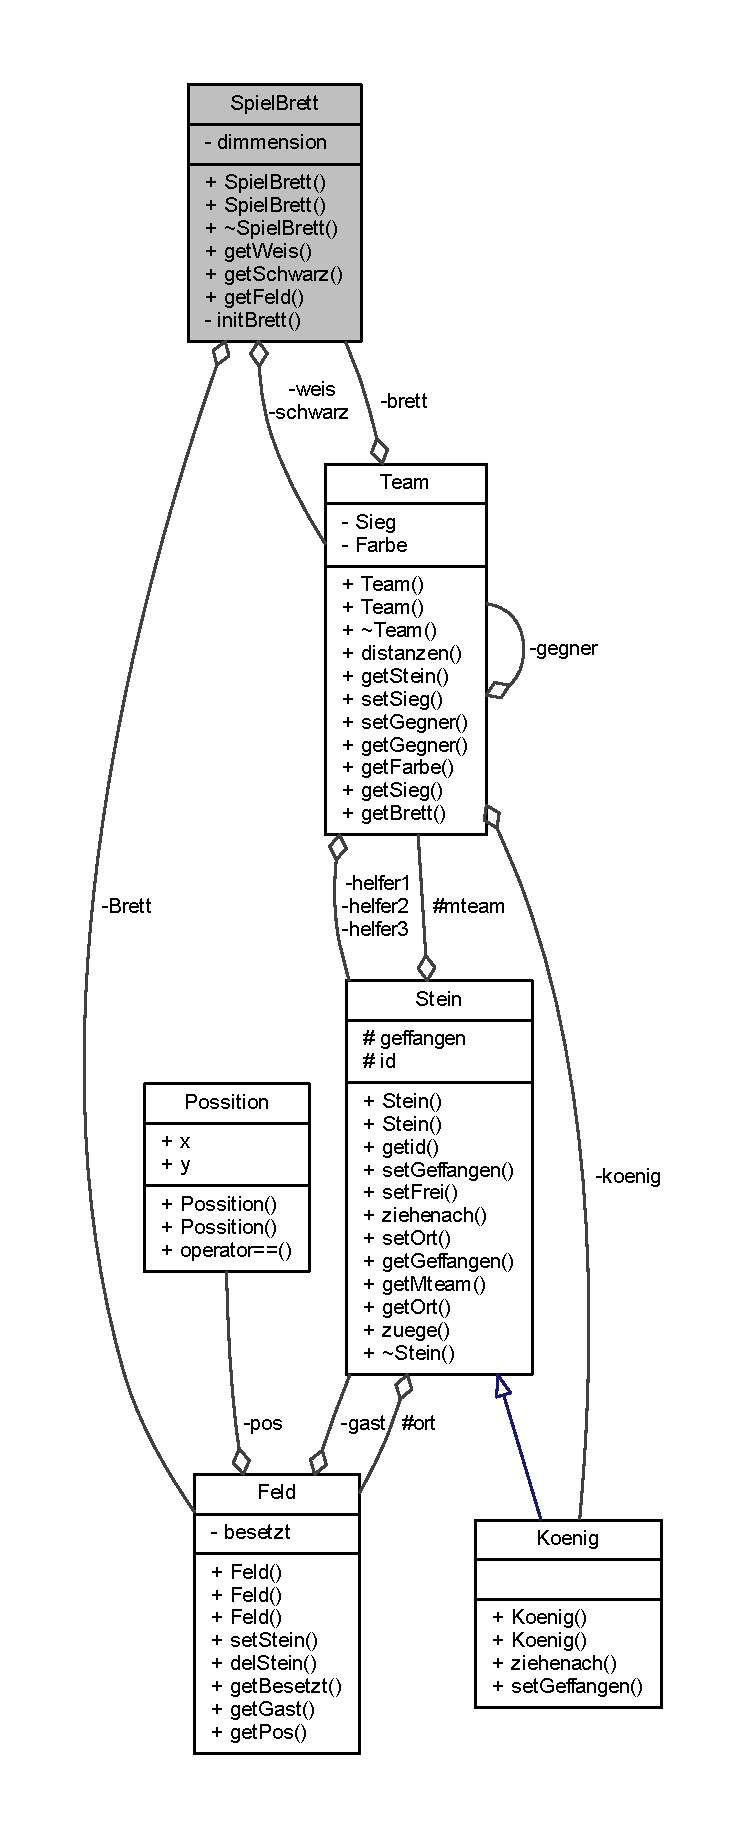
\includegraphics[height=550pt]{class_spiel_brett__coll__graph}
\end{center}
\end{figure}
\subsection*{Öffentliche Methoden}
\begin{DoxyCompactItemize}
\item 
\hyperlink{class_spiel_brett_abd1c86dc9518ff9c368b43d8c49db6c0}{Spiel\+Brett} ()
\item 
\hyperlink{class_spiel_brett_aa81d890cf06cc6c834f98cb0411d9026}{Spiel\+Brett} (const \hyperlink{class_spiel_brett}{Spiel\+Brett} \&sb)
\item 
\hyperlink{class_spiel_brett_ab61306e45606cab9ab9d073c43cf30f8}{$\sim$\+Spiel\+Brett} ()
\item 
\hyperlink{class_team}{Team} $\ast$ \hyperlink{class_spiel_brett_acb3a18d766bd52142672b8d0300d6686}{get\+Weis} () const 
\item 
\hyperlink{class_team}{Team} $\ast$ \hyperlink{class_spiel_brett_a30fb11863bee09200875119d15d282b1}{get\+Schwarz} () const 
\item 
\hyperlink{class_feld}{Feld} $\ast$ \hyperlink{class_spiel_brett_a6fc31b54e16797baf80285872ce2dab1}{get\+Feld} (int x, int y) const 
\end{DoxyCompactItemize}
\subsection*{Private Methoden}
\begin{DoxyCompactItemize}
\item 
void \hyperlink{class_spiel_brett_a1a4090a83c4c6fc7205ee80764bebcf0}{init\+Brett} ()
\end{DoxyCompactItemize}
\subsection*{Private Attribute}
\begin{DoxyCompactItemize}
\item 
\hyperlink{class_feld}{Feld} $\ast$$\ast$ \hyperlink{class_spiel_brett_a507b430b3d9f96db6eaa02b9dd9d5f99}{Brett} =nullptr
\item 
\hyperlink{class_team}{Team} $\ast$ \hyperlink{class_spiel_brett_afc28f676d2b3556b29adbf0ef32ba679}{schwarz} =nullptr
\item 
\hyperlink{class_team}{Team} $\ast$ \hyperlink{class_spiel_brett_aa5c83f7c16af3ea1c51d2ea9745875ac}{weis} =nullptr
\end{DoxyCompactItemize}
\subsection*{Statische, private Attribute}
\begin{DoxyCompactItemize}
\item 
static const short int \hyperlink{class_spiel_brett_a428ac783e187cd6a25f15b833555312a}{dimmension} = 8
\end{DoxyCompactItemize}


\subsection{Beschreibung der Konstruktoren und Destruktoren}
\hypertarget{class_spiel_brett_abd1c86dc9518ff9c368b43d8c49db6c0}{}\index{Spiel\+Brett@{Spiel\+Brett}!Spiel\+Brett@{Spiel\+Brett}}
\index{Spiel\+Brett@{Spiel\+Brett}!Spiel\+Brett@{Spiel\+Brett}}
\subsubsection[{Spiel\+Brett}]{\setlength{\rightskip}{0pt plus 5cm}Spiel\+Brett\+::\+Spiel\+Brett (
\begin{DoxyParamCaption}
{}
\end{DoxyParamCaption}
)}\label{class_spiel_brett_abd1c86dc9518ff9c368b43d8c49db6c0}
\hyperlink{class_spiel_brett_a1a4090a83c4c6fc7205ee80764bebcf0}{init\+Brett()} Erzeugt das 8x8 großes \hyperlink{class_feld}{Feld}. 

Hier ist ein Graph, der zeigt, was diese Funktion aufruft\+:\nopagebreak
\begin{figure}[H]
\begin{center}
\leavevmode
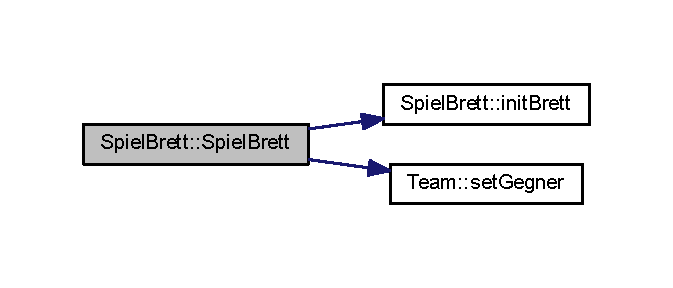
\includegraphics[width=323pt]{class_spiel_brett_abd1c86dc9518ff9c368b43d8c49db6c0_cgraph}
\end{center}
\end{figure}


\hypertarget{class_spiel_brett_aa81d890cf06cc6c834f98cb0411d9026}{}\index{Spiel\+Brett@{Spiel\+Brett}!Spiel\+Brett@{Spiel\+Brett}}
\index{Spiel\+Brett@{Spiel\+Brett}!Spiel\+Brett@{Spiel\+Brett}}
\subsubsection[{Spiel\+Brett}]{\setlength{\rightskip}{0pt plus 5cm}Spiel\+Brett\+::\+Spiel\+Brett (
\begin{DoxyParamCaption}
\item[{const {\bf Spiel\+Brett} \&}]{sb}
\end{DoxyParamCaption}
)}\label{class_spiel_brett_aa81d890cf06cc6c834f98cb0411d9026}
\hyperlink{class_spiel_brett_abd1c86dc9518ff9c368b43d8c49db6c0}{Spiel\+Brett()} Beinhaltet die Startaufstellung. 

Hier ist ein Graph, der zeigt, was diese Funktion aufruft\+:\nopagebreak
\begin{figure}[H]
\begin{center}
\leavevmode
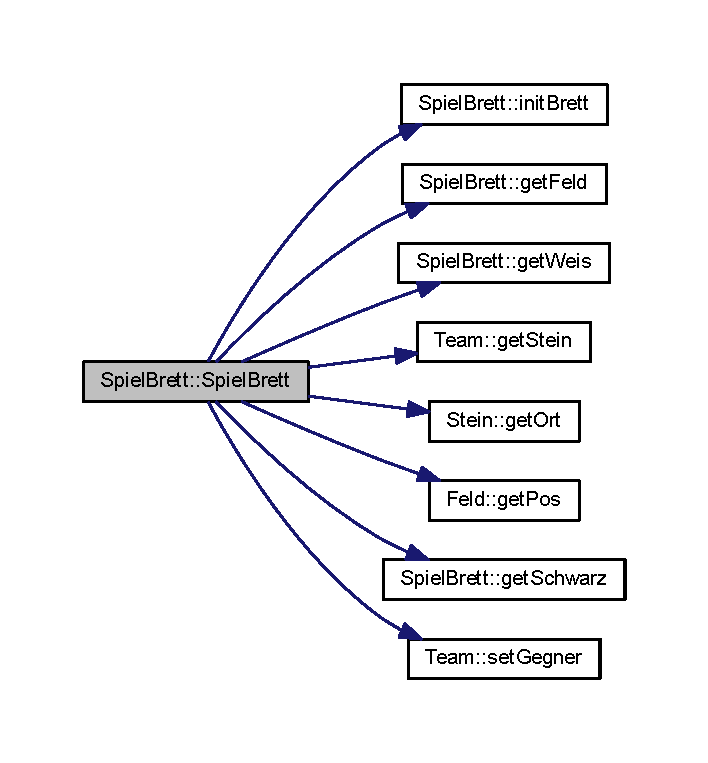
\includegraphics[width=340pt]{class_spiel_brett_aa81d890cf06cc6c834f98cb0411d9026_cgraph}
\end{center}
\end{figure}


\hypertarget{class_spiel_brett_ab61306e45606cab9ab9d073c43cf30f8}{}\index{Spiel\+Brett@{Spiel\+Brett}!````~Spiel\+Brett@{$\sim$\+Spiel\+Brett}}
\index{````~Spiel\+Brett@{$\sim$\+Spiel\+Brett}!Spiel\+Brett@{Spiel\+Brett}}
\subsubsection[{$\sim$\+Spiel\+Brett}]{\setlength{\rightskip}{0pt plus 5cm}Spiel\+Brett\+::$\sim$\+Spiel\+Brett (
\begin{DoxyParamCaption}
{}
\end{DoxyParamCaption}
)}\label{class_spiel_brett_ab61306e45606cab9ab9d073c43cf30f8}
\hyperlink{class_spiel_brett}{Spiel\+Brett} (const \hyperlink{class_spiel_brett}{Spiel\+Brett} \&sb) Verweißt auf die Pointer, der einzelnen Spielsteine. 

\subsection{Dokumentation der Elementfunktionen}
\hypertarget{class_spiel_brett_a6fc31b54e16797baf80285872ce2dab1}{}\index{Spiel\+Brett@{Spiel\+Brett}!get\+Feld@{get\+Feld}}
\index{get\+Feld@{get\+Feld}!Spiel\+Brett@{Spiel\+Brett}}
\subsubsection[{get\+Feld}]{\setlength{\rightskip}{0pt plus 5cm}{\bf Feld} $\ast$ Spiel\+Brett\+::get\+Feld (
\begin{DoxyParamCaption}
\item[{int}]{x, }
\item[{int}]{y}
\end{DoxyParamCaption}
) const}\label{class_spiel_brett_a6fc31b54e16797baf80285872ce2dab1}
\hyperlink{class_spiel_brett_a30fb11863bee09200875119d15d282b1}{get\+Schwarz()} Kennzeichnet die schwarzen Steine.

\begin{DoxyReturn}{Rückgabe}
schwarz 
\end{DoxyReturn}
\hypertarget{class_spiel_brett_a30fb11863bee09200875119d15d282b1}{}\index{Spiel\+Brett@{Spiel\+Brett}!get\+Schwarz@{get\+Schwarz}}
\index{get\+Schwarz@{get\+Schwarz}!Spiel\+Brett@{Spiel\+Brett}}
\subsubsection[{get\+Schwarz}]{\setlength{\rightskip}{0pt plus 5cm}{\bf Team} $\ast$ Spiel\+Brett\+::get\+Schwarz (
\begin{DoxyParamCaption}
{}
\end{DoxyParamCaption}
) const}\label{class_spiel_brett_a30fb11863bee09200875119d15d282b1}
\hyperlink{class_spiel_brett_acb3a18d766bd52142672b8d0300d6686}{get\+Weis()} Kennzeichnet die weißen Steine.

\begin{DoxyReturn}{Rückgabe}
weiß 
\end{DoxyReturn}
\hypertarget{class_spiel_brett_acb3a18d766bd52142672b8d0300d6686}{}\index{Spiel\+Brett@{Spiel\+Brett}!get\+Weis@{get\+Weis}}
\index{get\+Weis@{get\+Weis}!Spiel\+Brett@{Spiel\+Brett}}
\subsubsection[{get\+Weis}]{\setlength{\rightskip}{0pt plus 5cm}{\bf Team} $\ast$ Spiel\+Brett\+::get\+Weis (
\begin{DoxyParamCaption}
{}
\end{DoxyParamCaption}
) const}\label{class_spiel_brett_acb3a18d766bd52142672b8d0300d6686}
$\sim$\+Spiel\+Brett Destruktor des Spiels \hypertarget{class_spiel_brett_a1a4090a83c4c6fc7205ee80764bebcf0}{}\index{Spiel\+Brett@{Spiel\+Brett}!init\+Brett@{init\+Brett}}
\index{init\+Brett@{init\+Brett}!Spiel\+Brett@{Spiel\+Brett}}
\subsubsection[{init\+Brett}]{\setlength{\rightskip}{0pt plus 5cm}void Spiel\+Brett\+::init\+Brett (
\begin{DoxyParamCaption}
{}
\end{DoxyParamCaption}
)\hspace{0.3cm}{\ttfamily [private]}}\label{class_spiel_brett_a1a4090a83c4c6fc7205ee80764bebcf0}


\subsection{Dokumentation der Datenelemente}
\hypertarget{class_spiel_brett_a507b430b3d9f96db6eaa02b9dd9d5f99}{}\index{Spiel\+Brett@{Spiel\+Brett}!Brett@{Brett}}
\index{Brett@{Brett}!Spiel\+Brett@{Spiel\+Brett}}
\subsubsection[{Brett}]{\setlength{\rightskip}{0pt plus 5cm}{\bf Feld}$\ast$$\ast$ Spiel\+Brett\+::\+Brett =nullptr\hspace{0.3cm}{\ttfamily [private]}}\label{class_spiel_brett_a507b430b3d9f96db6eaa02b9dd9d5f99}
\hypertarget{class_spiel_brett_a428ac783e187cd6a25f15b833555312a}{}\index{Spiel\+Brett@{Spiel\+Brett}!dimmension@{dimmension}}
\index{dimmension@{dimmension}!Spiel\+Brett@{Spiel\+Brett}}
\subsubsection[{dimmension}]{\setlength{\rightskip}{0pt plus 5cm}const short int Spiel\+Brett\+::dimmension = 8\hspace{0.3cm}{\ttfamily [static]}, {\ttfamily [private]}}\label{class_spiel_brett_a428ac783e187cd6a25f15b833555312a}
\hypertarget{class_spiel_brett_afc28f676d2b3556b29adbf0ef32ba679}{}\index{Spiel\+Brett@{Spiel\+Brett}!schwarz@{schwarz}}
\index{schwarz@{schwarz}!Spiel\+Brett@{Spiel\+Brett}}
\subsubsection[{schwarz}]{\setlength{\rightskip}{0pt plus 5cm}{\bf Team}$\ast$ Spiel\+Brett\+::schwarz =nullptr\hspace{0.3cm}{\ttfamily [private]}}\label{class_spiel_brett_afc28f676d2b3556b29adbf0ef32ba679}
\hypertarget{class_spiel_brett_aa5c83f7c16af3ea1c51d2ea9745875ac}{}\index{Spiel\+Brett@{Spiel\+Brett}!weis@{weis}}
\index{weis@{weis}!Spiel\+Brett@{Spiel\+Brett}}
\subsubsection[{weis}]{\setlength{\rightskip}{0pt plus 5cm}{\bf Team} $\ast$ Spiel\+Brett\+::weis =nullptr\hspace{0.3cm}{\ttfamily [private]}}\label{class_spiel_brett_aa5c83f7c16af3ea1c51d2ea9745875ac}


Die Dokumentation für diese Klasse wurde erzeugt aufgrund der Dateien\+:\begin{DoxyCompactItemize}
\item 
\hyperlink{_spiel_brett_8h}{Spiel\+Brett.\+h}\item 
\hyperlink{_spiel_brett_8cpp}{Spiel\+Brett.\+cpp}\end{DoxyCompactItemize}

\hypertarget{class_sr_h}{}\section{Sr\+H Klassenreferenz}
\label{class_sr_h}\index{Sr\+H@{Sr\+H}}


{\ttfamily \#include $<$Sr\+H.\+h$>$}



Klassendiagramm für Sr\+H\+:\nopagebreak
\begin{figure}[H]
\begin{center}
\leavevmode
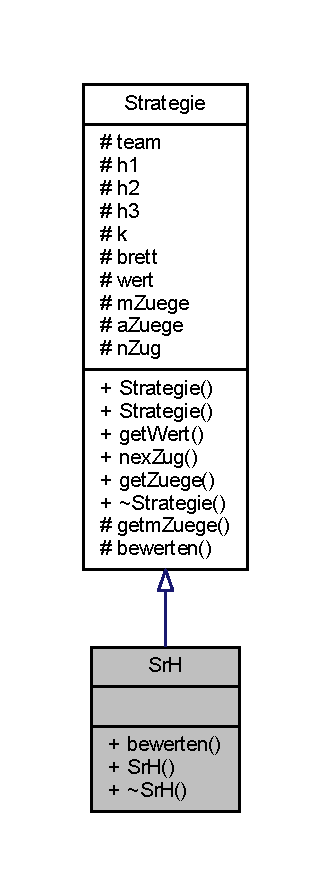
\includegraphics[width=159pt]{class_sr_h__inherit__graph}
\end{center}
\end{figure}


Zusammengehörigkeiten von Sr\+H\+:\nopagebreak
\begin{figure}[H]
\begin{center}
\leavevmode
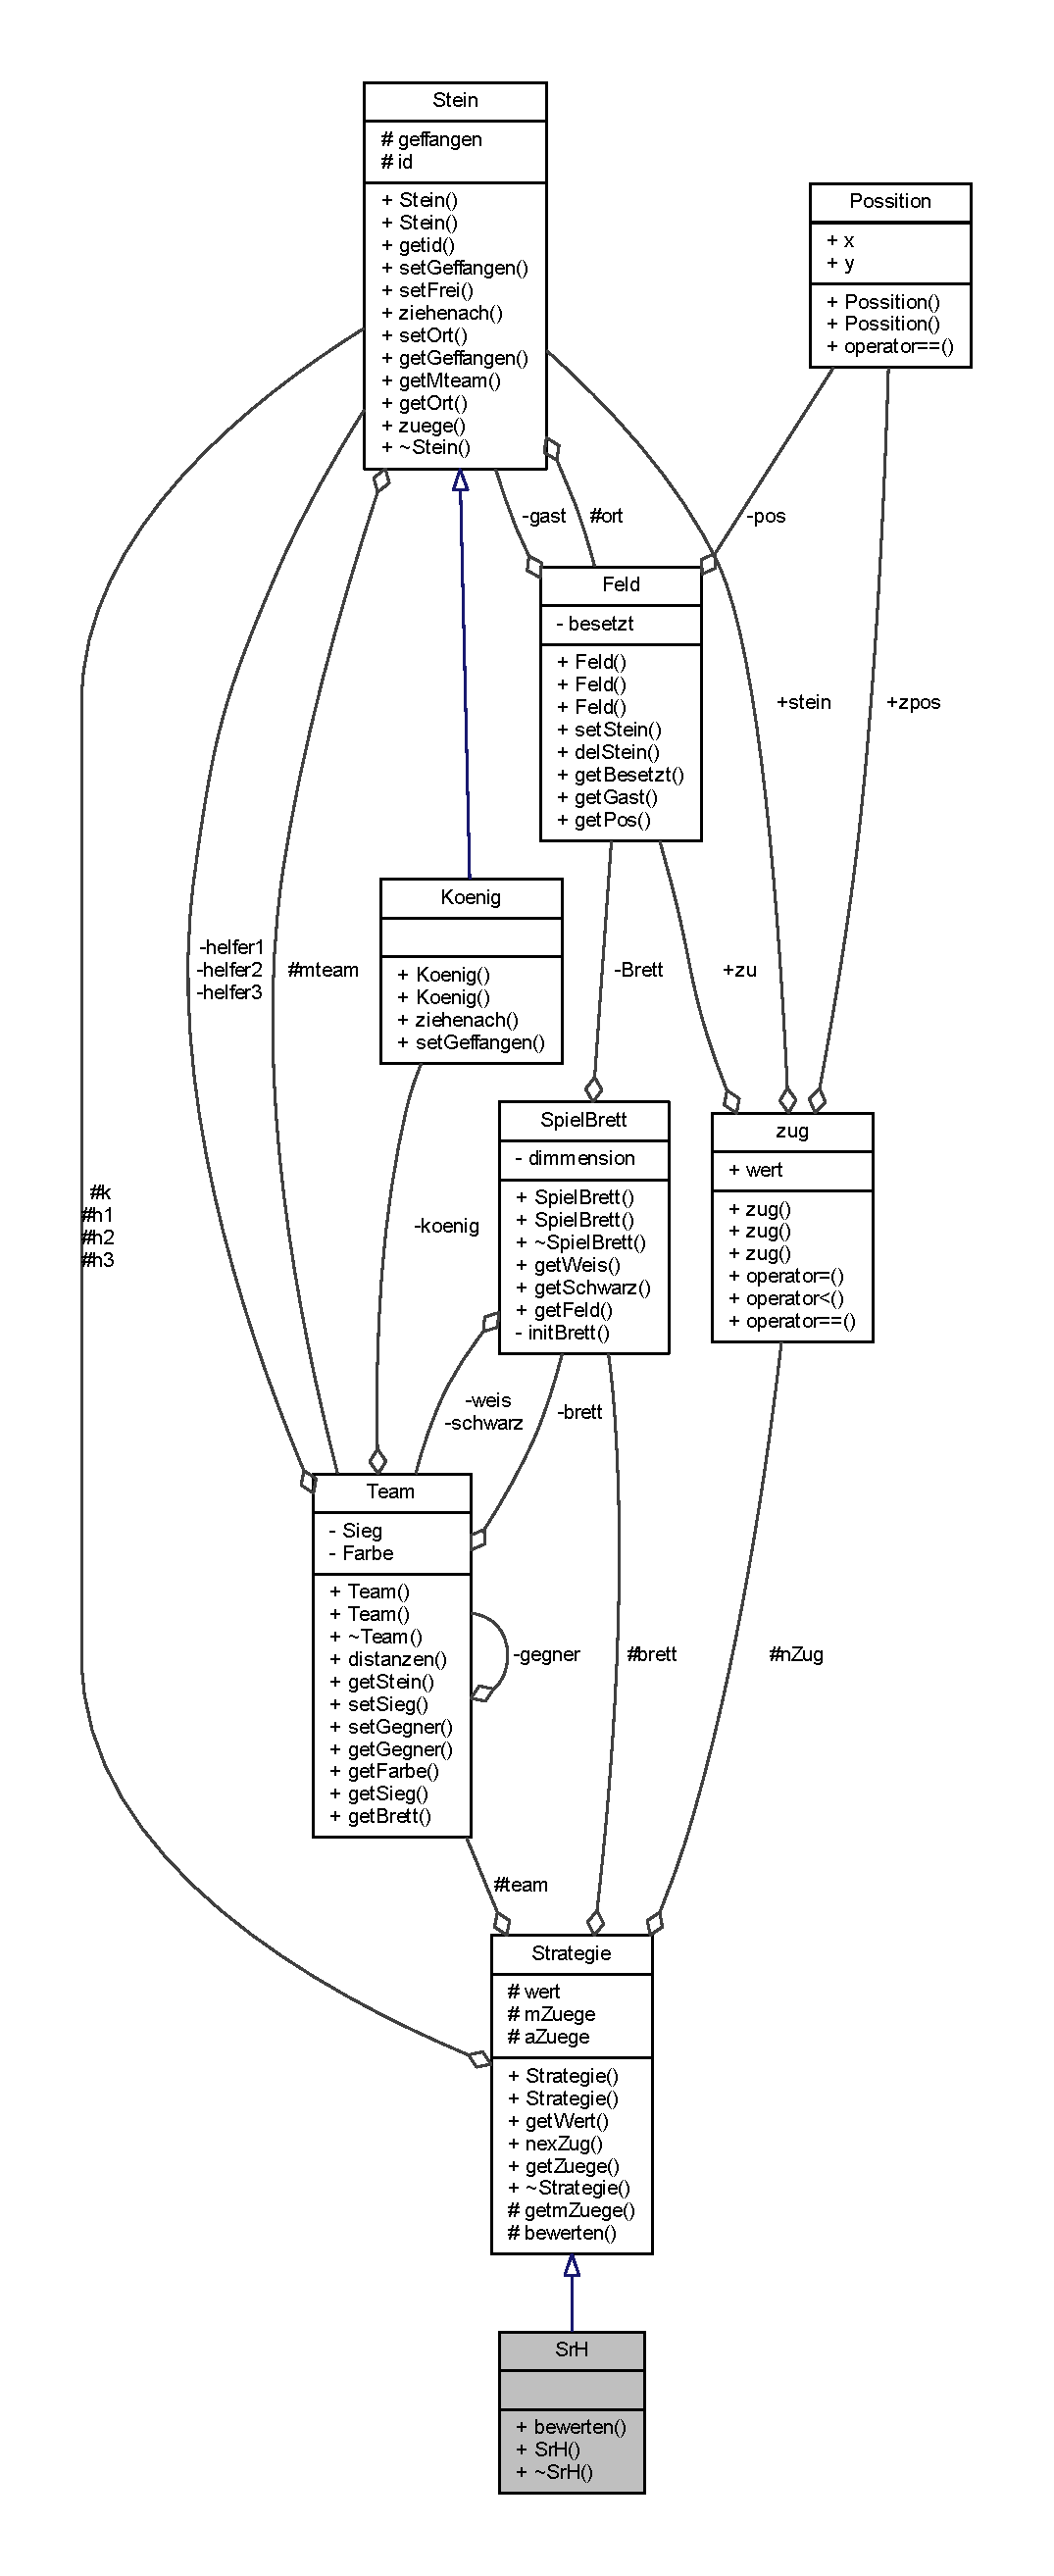
\includegraphics[height=550pt]{class_sr_h__coll__graph}
\end{center}
\end{figure}
\subsection*{Öffentliche Methoden}
\begin{DoxyCompactItemize}
\item 
virtual void \hyperlink{class_sr_h_a55d77665881d6810fbde7d761ecbb02c}{bewerten} () override
\item 
\hyperlink{class_sr_h_a82cf641600edd8043d09c03478fac61e}{Sr\+H} (\hyperlink{class_team}{Team} \&\hyperlink{class_strategie_a4f55e74f189ec8c6df88a57119fb3def}{team}, \hyperlink{class_spiel_brett}{Spiel\+Brett} \&b)
\item 
virtual \hyperlink{class_sr_h_ac7f7f95344ee9e1517f8f5dcb515cc40}{$\sim$\+Sr\+H} ()
\end{DoxyCompactItemize}
\subsection*{Weitere Geerbte Elemente}


\subsection{Ausführliche Beschreibung}
class \hyperlink{class_sr_h}{Sr\+H} (\hyperlink{class_strategie}{Strategie} rette Helfer) Ist eine Ableitung der abstrakten Klasse \hyperlink{class_strategie}{Strategie}. \subparagraph*{}

Diese \hyperlink{class_strategie}{Strategie} sorgt dafuer, dass der \hyperlink{class_koenig}{Koenig} teameigene festgesetzte/gefangene Helfer befreit. Dies tut er allerdings nach Moeglichkeit erst dann, wenn sie sich auch in unmittelbarer Umgebung befinden, da der \hyperlink{class_koenig}{Koenig} selber eine sehr defensive Rolle im Spielverlauf einnimmt. \subparagraph*{}

Ueberschreibt/implementiert die Methode \hyperlink{class_sr_h_a55d77665881d6810fbde7d761ecbb02c}{bewerten()}; 
\begin{DoxyParams}{Parameter}
{\em \&team} & Referenz auf Instanz von \hyperlink{class_team}{Team} \\
\hline
{\em \&b} & Referenz auf Instanz von \hyperlink{class_spiel_brett}{Spiel\+Brett} \\
\hline
\end{DoxyParams}


\subsection{Beschreibung der Konstruktoren und Destruktoren}
\hypertarget{class_sr_h_a82cf641600edd8043d09c03478fac61e}{}\index{Sr\+H@{Sr\+H}!Sr\+H@{Sr\+H}}
\index{Sr\+H@{Sr\+H}!Sr\+H@{Sr\+H}}
\subsubsection[{Sr\+H}]{\setlength{\rightskip}{0pt plus 5cm}Sr\+H\+::\+Sr\+H (
\begin{DoxyParamCaption}
\item[{{\bf Team} \&}]{team, }
\item[{{\bf Spiel\+Brett} \&}]{b}
\end{DoxyParamCaption}
)}\label{class_sr_h_a82cf641600edd8043d09c03478fac61e}
\hypertarget{class_sr_h_ac7f7f95344ee9e1517f8f5dcb515cc40}{}\index{Sr\+H@{Sr\+H}!````~Sr\+H@{$\sim$\+Sr\+H}}
\index{````~Sr\+H@{$\sim$\+Sr\+H}!Sr\+H@{Sr\+H}}
\subsubsection[{$\sim$\+Sr\+H}]{\setlength{\rightskip}{0pt plus 5cm}Sr\+H\+::$\sim$\+Sr\+H (
\begin{DoxyParamCaption}
{}
\end{DoxyParamCaption}
)\hspace{0.3cm}{\ttfamily [virtual]}}\label{class_sr_h_ac7f7f95344ee9e1517f8f5dcb515cc40}


\subsection{Dokumentation der Elementfunktionen}
\hypertarget{class_sr_h_a55d77665881d6810fbde7d761ecbb02c}{}\index{Sr\+H@{Sr\+H}!bewerten@{bewerten}}
\index{bewerten@{bewerten}!Sr\+H@{Sr\+H}}
\subsubsection[{bewerten}]{\setlength{\rightskip}{0pt plus 5cm}void Sr\+H\+::bewerten (
\begin{DoxyParamCaption}
{}
\end{DoxyParamCaption}
)\hspace{0.3cm}{\ttfamily [override]}, {\ttfamily [virtual]}}\label{class_sr_h_a55d77665881d6810fbde7d761ecbb02c}


Implementiert \hyperlink{class_strategie_a6e11413c1c8e4ca8bd0bcac21be3c1bf}{Strategie}.



Hier ist ein Graph, der zeigt, was diese Funktion aufruft\+:\nopagebreak
\begin{figure}[H]
\begin{center}
\leavevmode
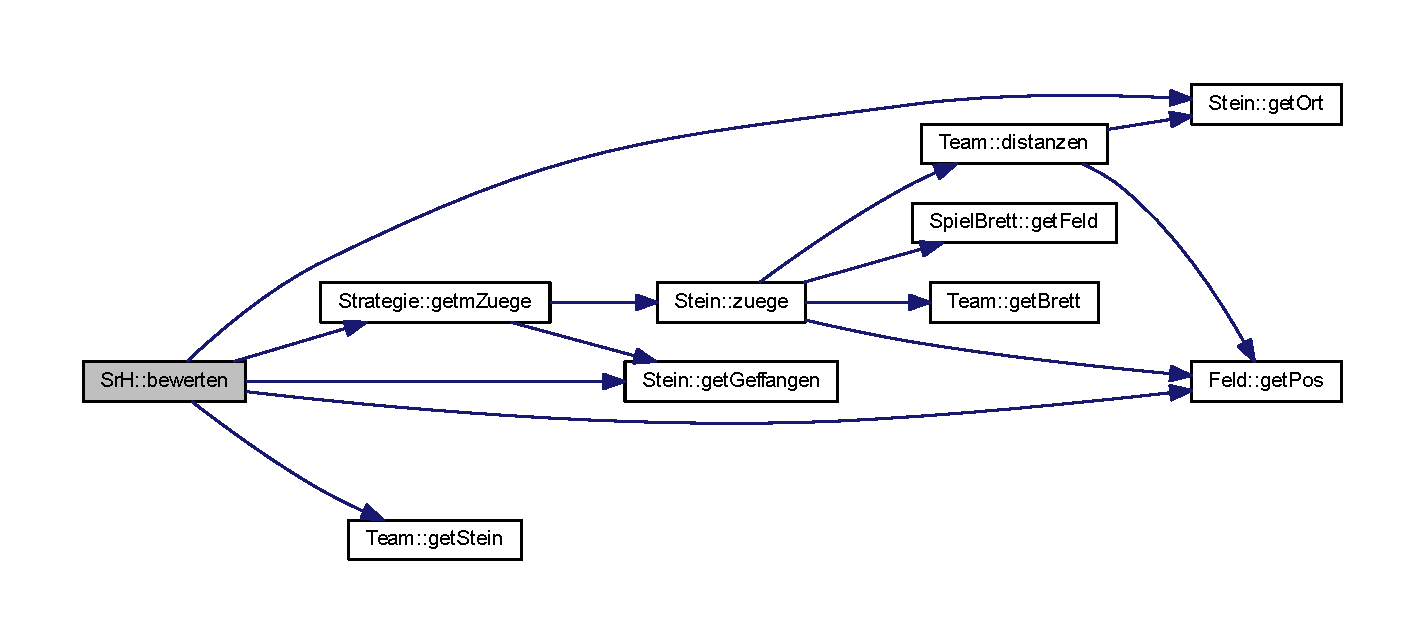
\includegraphics[width=350pt]{class_sr_h_a55d77665881d6810fbde7d761ecbb02c_cgraph}
\end{center}
\end{figure}




Die Dokumentation für diese Klasse wurde erzeugt aufgrund der Dateien\+:\begin{DoxyCompactItemize}
\item 
\hyperlink{_sr_h_8h}{Sr\+H.\+h}\item 
\hyperlink{_sr_h_8cpp}{Sr\+H.\+cpp}\end{DoxyCompactItemize}

\hypertarget{class_ss_k}{}\section{Ss\+K Klassenreferenz}
\label{class_ss_k}\index{Ss\+K@{Ss\+K}}


{\ttfamily \#include $<$Ss\+K.\+h$>$}



Klassendiagramm für Ss\+K\+:\nopagebreak
\begin{figure}[H]
\begin{center}
\leavevmode
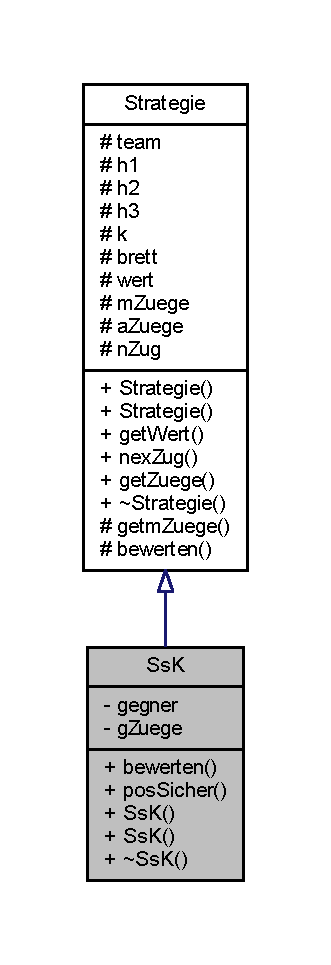
\includegraphics[width=159pt]{class_ss_k__inherit__graph}
\end{center}
\end{figure}


Zusammengehörigkeiten von Ss\+K\+:\nopagebreak
\begin{figure}[H]
\begin{center}
\leavevmode
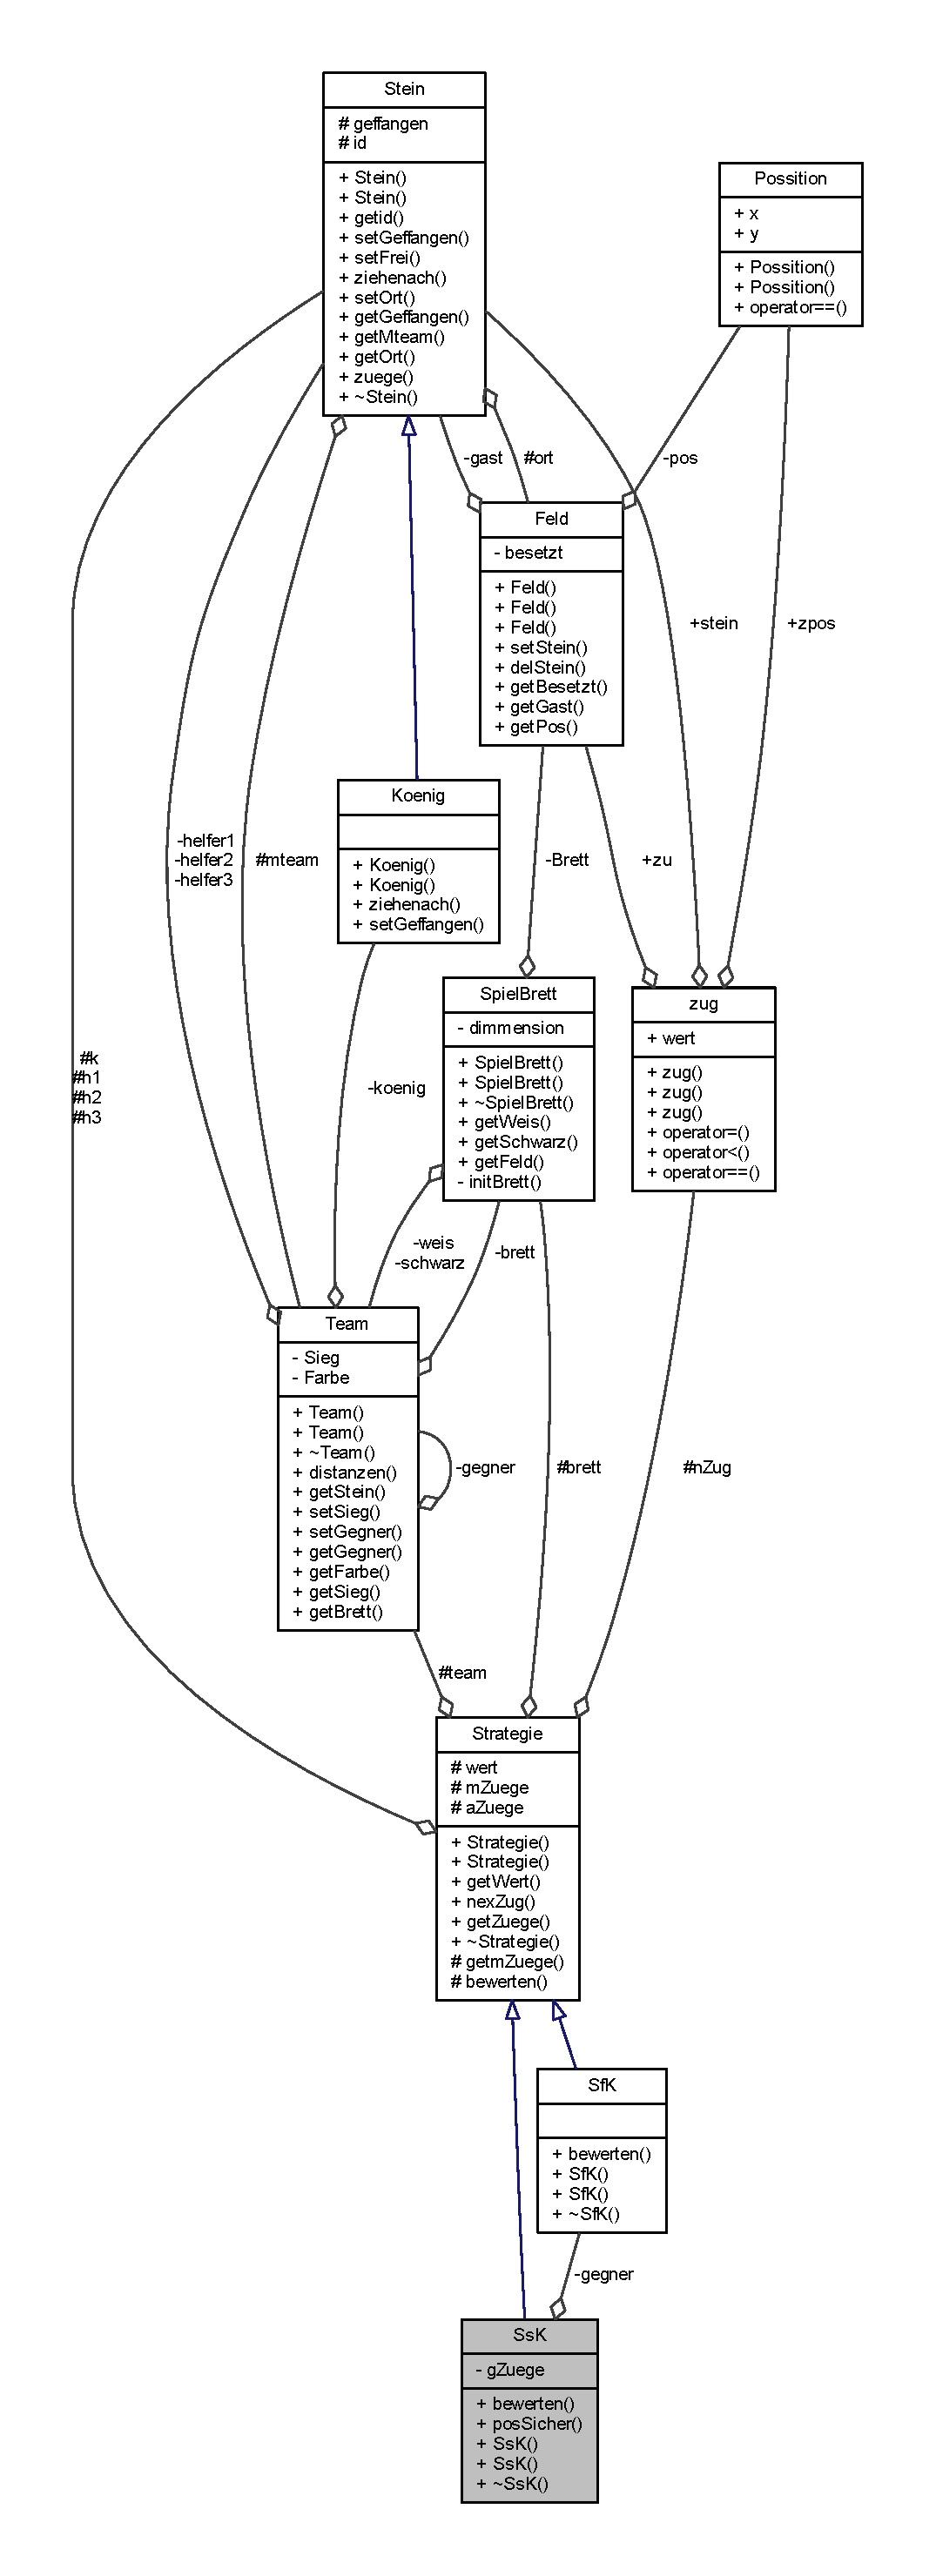
\includegraphics[height=550pt]{class_ss_k__coll__graph}
\end{center}
\end{figure}
\subsection*{Öffentliche Methoden}
\begin{DoxyCompactItemize}
\item 
virtual void \hyperlink{class_ss_k_aac922686e66332aae431ec05d06937a0}{bewerten} () override
\item 
bool \hyperlink{class_ss_k_a7034ff44a447cef0d24117e9a1fa9fef}{pos\+Sicher} (\hyperlink{struct_possition}{Possition} p)
\item 
\hyperlink{class_ss_k_a2cb13922fb8c0bdbad4dd36f98c0448b}{Ss\+K} (\hyperlink{class_team}{Team} \&\hyperlink{class_strategie_a4f55e74f189ec8c6df88a57119fb3def}{team}, \hyperlink{class_spiel_brett}{Spiel\+Brett} \&b)
\item 
\hyperlink{class_ss_k_a24d667d15c076686914ad331b2306f14}{Ss\+K} ()
\item 
virtual \hyperlink{class_ss_k_a3912f76c805a0d1810e0ab0c12bf49b4}{$\sim$\+Ss\+K} ()
\end{DoxyCompactItemize}
\subsection*{Private Attribute}
\begin{DoxyCompactItemize}
\item 
\hyperlink{class_sf_k}{Sf\+K} \hyperlink{class_ss_k_a4c117e68ae76434738995801a4a1fbcc}{gegner}
\item 
std\+::vector$<$ \hyperlink{structzug}{zug} $>$ \hyperlink{class_ss_k_af5cfdbc60256434dbb73e61e737e056a}{g\+Zuege}
\end{DoxyCompactItemize}
\subsection*{Weitere Geerbte Elemente}


\subsection{Ausführliche Beschreibung}
class \hyperlink{class_ss_k}{Ss\+K} (\hyperlink{class_strategie}{Strategie} schuetze \hyperlink{class_koenig}{Koenig}) Ist eine Ableitung der abstrakten Klasse \hyperlink{class_strategie}{Strategie}. \subparagraph*{}

Diese \hyperlink{class_strategie}{Strategie} sorgt dafuer, dass der teameigene \hyperlink{class_koenig}{Koenig} vor festsetzen/gefangen nehmen durch feindliche Spielfiguren geschuetzt wird. Zu beobachten ist hierbei das fangen von gegnerischen Spielfiguren, sobald sie dem König zu nahe kommen. Auch der \hyperlink{class_koenig}{Koenig} selber nimmt ein sehr defensives Verhalten an und haelt sich von den Gegnern fern, um ein fruehzeitiges Ableben zu verhindern. \subparagraph*{}

Ueberschreibt/implementiert die Methode \hyperlink{class_ss_k_aac922686e66332aae431ec05d06937a0}{bewerten()}; 
\begin{DoxyParams}{Parameter}
{\em \&team} & Referenz auf Instanz von \hyperlink{class_team}{Team} \\
\hline
{\em \&b} & Referenz auf Instanz von \hyperlink{class_spiel_brett}{Spiel\+Brett} \\
\hline
\end{DoxyParams}


\subsection{Beschreibung der Konstruktoren und Destruktoren}
\hypertarget{class_ss_k_a2cb13922fb8c0bdbad4dd36f98c0448b}{}\index{Ss\+K@{Ss\+K}!Ss\+K@{Ss\+K}}
\index{Ss\+K@{Ss\+K}!Ss\+K@{Ss\+K}}
\subsubsection[{Ss\+K}]{\setlength{\rightskip}{0pt plus 5cm}Ss\+K\+::\+Ss\+K (
\begin{DoxyParamCaption}
\item[{{\bf Team} \&}]{team, }
\item[{{\bf Spiel\+Brett} \&}]{b}
\end{DoxyParamCaption}
)}\label{class_ss_k_a2cb13922fb8c0bdbad4dd36f98c0448b}
\hypertarget{class_ss_k_a24d667d15c076686914ad331b2306f14}{}\index{Ss\+K@{Ss\+K}!Ss\+K@{Ss\+K}}
\index{Ss\+K@{Ss\+K}!Ss\+K@{Ss\+K}}
\subsubsection[{Ss\+K}]{\setlength{\rightskip}{0pt plus 5cm}Ss\+K\+::\+Ss\+K (
\begin{DoxyParamCaption}
{}
\end{DoxyParamCaption}
)}\label{class_ss_k_a24d667d15c076686914ad331b2306f14}
\hypertarget{class_ss_k_a3912f76c805a0d1810e0ab0c12bf49b4}{}\index{Ss\+K@{Ss\+K}!````~Ss\+K@{$\sim$\+Ss\+K}}
\index{````~Ss\+K@{$\sim$\+Ss\+K}!Ss\+K@{Ss\+K}}
\subsubsection[{$\sim$\+Ss\+K}]{\setlength{\rightskip}{0pt plus 5cm}Ss\+K\+::$\sim$\+Ss\+K (
\begin{DoxyParamCaption}
{}
\end{DoxyParamCaption}
)\hspace{0.3cm}{\ttfamily [virtual]}}\label{class_ss_k_a3912f76c805a0d1810e0ab0c12bf49b4}


\subsection{Dokumentation der Elementfunktionen}
\hypertarget{class_ss_k_aac922686e66332aae431ec05d06937a0}{}\index{Ss\+K@{Ss\+K}!bewerten@{bewerten}}
\index{bewerten@{bewerten}!Ss\+K@{Ss\+K}}
\subsubsection[{bewerten}]{\setlength{\rightskip}{0pt plus 5cm}void Ss\+K\+::bewerten (
\begin{DoxyParamCaption}
{}
\end{DoxyParamCaption}
)\hspace{0.3cm}{\ttfamily [override]}, {\ttfamily [virtual]}}\label{class_ss_k_aac922686e66332aae431ec05d06937a0}


Implementiert \hyperlink{class_strategie_a6e11413c1c8e4ca8bd0bcac21be3c1bf}{Strategie}.



Hier ist ein Graph, der zeigt, was diese Funktion aufruft\+:\nopagebreak
\begin{figure}[H]
\begin{center}
\leavevmode
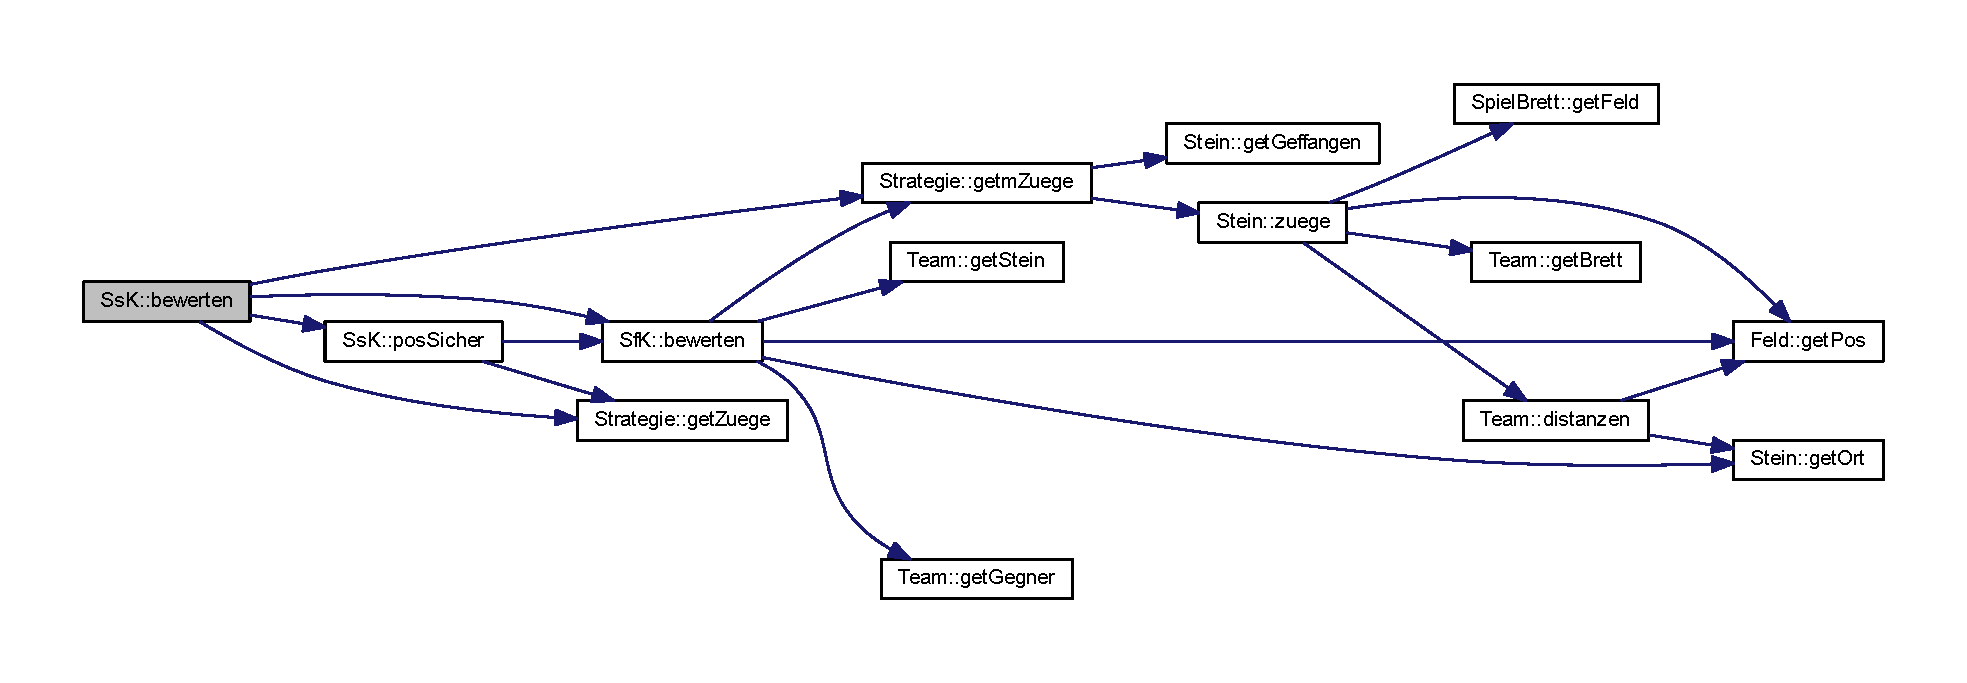
\includegraphics[width=350pt]{class_ss_k_aac922686e66332aae431ec05d06937a0_cgraph}
\end{center}
\end{figure}


\hypertarget{class_ss_k_a7034ff44a447cef0d24117e9a1fa9fef}{}\index{Ss\+K@{Ss\+K}!pos\+Sicher@{pos\+Sicher}}
\index{pos\+Sicher@{pos\+Sicher}!Ss\+K@{Ss\+K}}
\subsubsection[{pos\+Sicher}]{\setlength{\rightskip}{0pt plus 5cm}bool Ss\+K\+::pos\+Sicher (
\begin{DoxyParamCaption}
\item[{{\bf Possition}}]{p}
\end{DoxyParamCaption}
)}\label{class_ss_k_a7034ff44a447cef0d24117e9a1fa9fef}


Hier ist ein Graph, der zeigt, was diese Funktion aufruft\+:\nopagebreak
\begin{figure}[H]
\begin{center}
\leavevmode
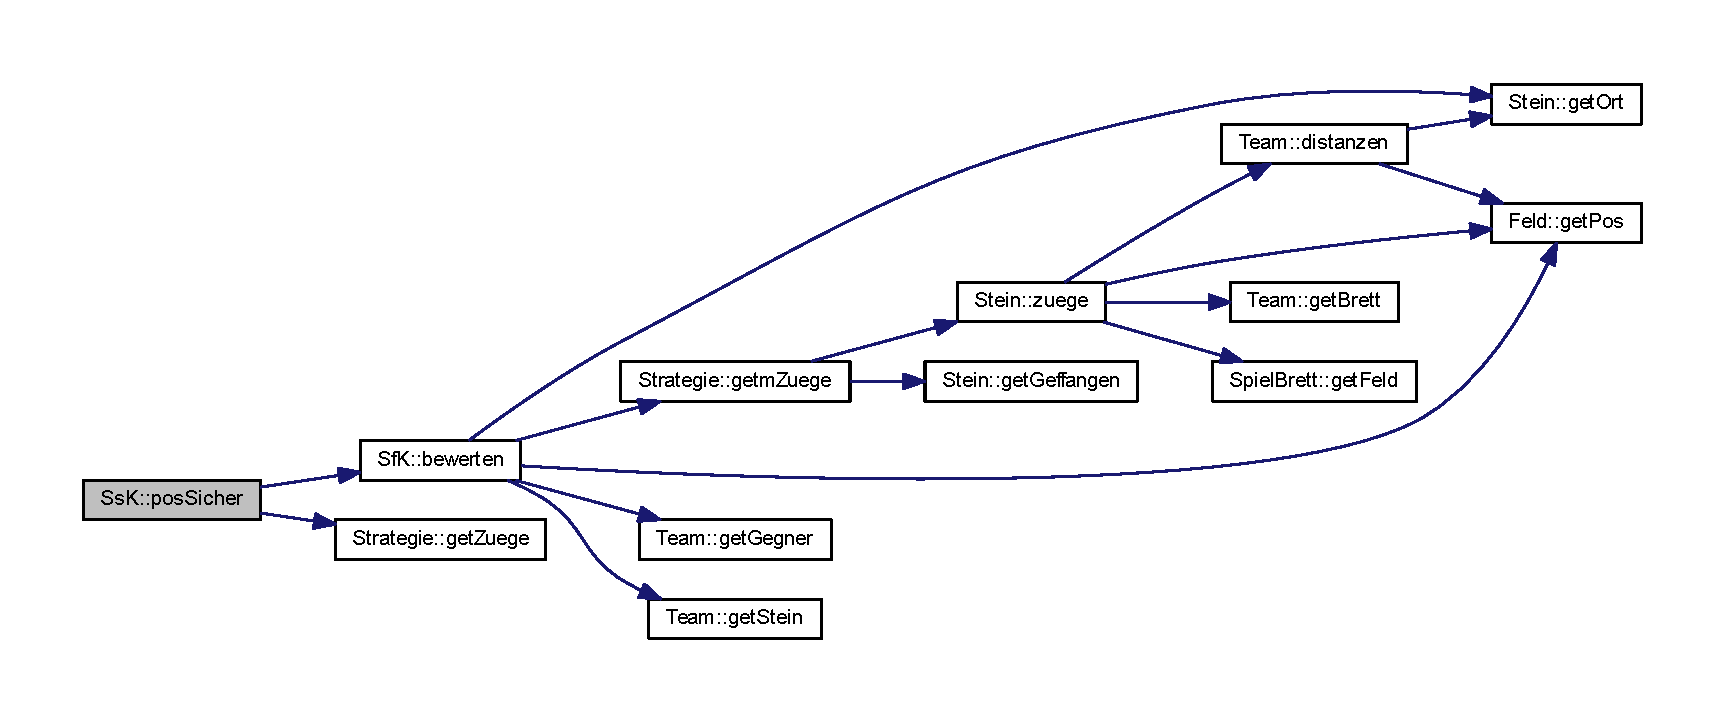
\includegraphics[width=350pt]{class_ss_k_a7034ff44a447cef0d24117e9a1fa9fef_cgraph}
\end{center}
\end{figure}




\subsection{Dokumentation der Datenelemente}
\hypertarget{class_ss_k_a4c117e68ae76434738995801a4a1fbcc}{}\index{Ss\+K@{Ss\+K}!gegner@{gegner}}
\index{gegner@{gegner}!Ss\+K@{Ss\+K}}
\subsubsection[{gegner}]{\setlength{\rightskip}{0pt plus 5cm}{\bf Sf\+K} Ss\+K\+::gegner\hspace{0.3cm}{\ttfamily [private]}}\label{class_ss_k_a4c117e68ae76434738995801a4a1fbcc}
\hypertarget{class_ss_k_af5cfdbc60256434dbb73e61e737e056a}{}\index{Ss\+K@{Ss\+K}!g\+Zuege@{g\+Zuege}}
\index{g\+Zuege@{g\+Zuege}!Ss\+K@{Ss\+K}}
\subsubsection[{g\+Zuege}]{\setlength{\rightskip}{0pt plus 5cm}std\+::vector$<${\bf zug}$>$ Ss\+K\+::g\+Zuege\hspace{0.3cm}{\ttfamily [private]}}\label{class_ss_k_af5cfdbc60256434dbb73e61e737e056a}


Die Dokumentation für diese Klasse wurde erzeugt aufgrund der Dateien\+:\begin{DoxyCompactItemize}
\item 
\hyperlink{_ss_k_8h}{Ss\+K.\+h}\item 
\hyperlink{_ss_k_8cpp}{Ss\+K.\+cpp}\end{DoxyCompactItemize}

\hypertarget{class_stein}{}\section{Stein Klassenreferenz}
\label{class_stein}\index{Stein@{Stein}}


{\ttfamily \#include $<$Stein.\+h$>$}



Klassendiagramm für Stein\+:\nopagebreak
\begin{figure}[H]
\begin{center}
\leavevmode
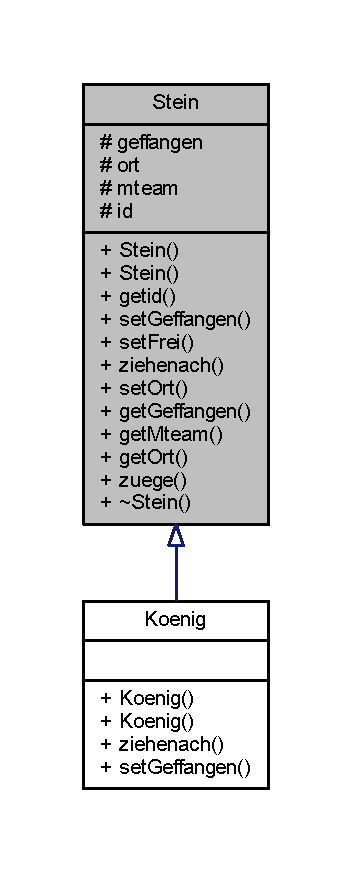
\includegraphics[width=169pt]{class_stein__inherit__graph}
\end{center}
\end{figure}


Zusammengehörigkeiten von Stein\+:\nopagebreak
\begin{figure}[H]
\begin{center}
\leavevmode
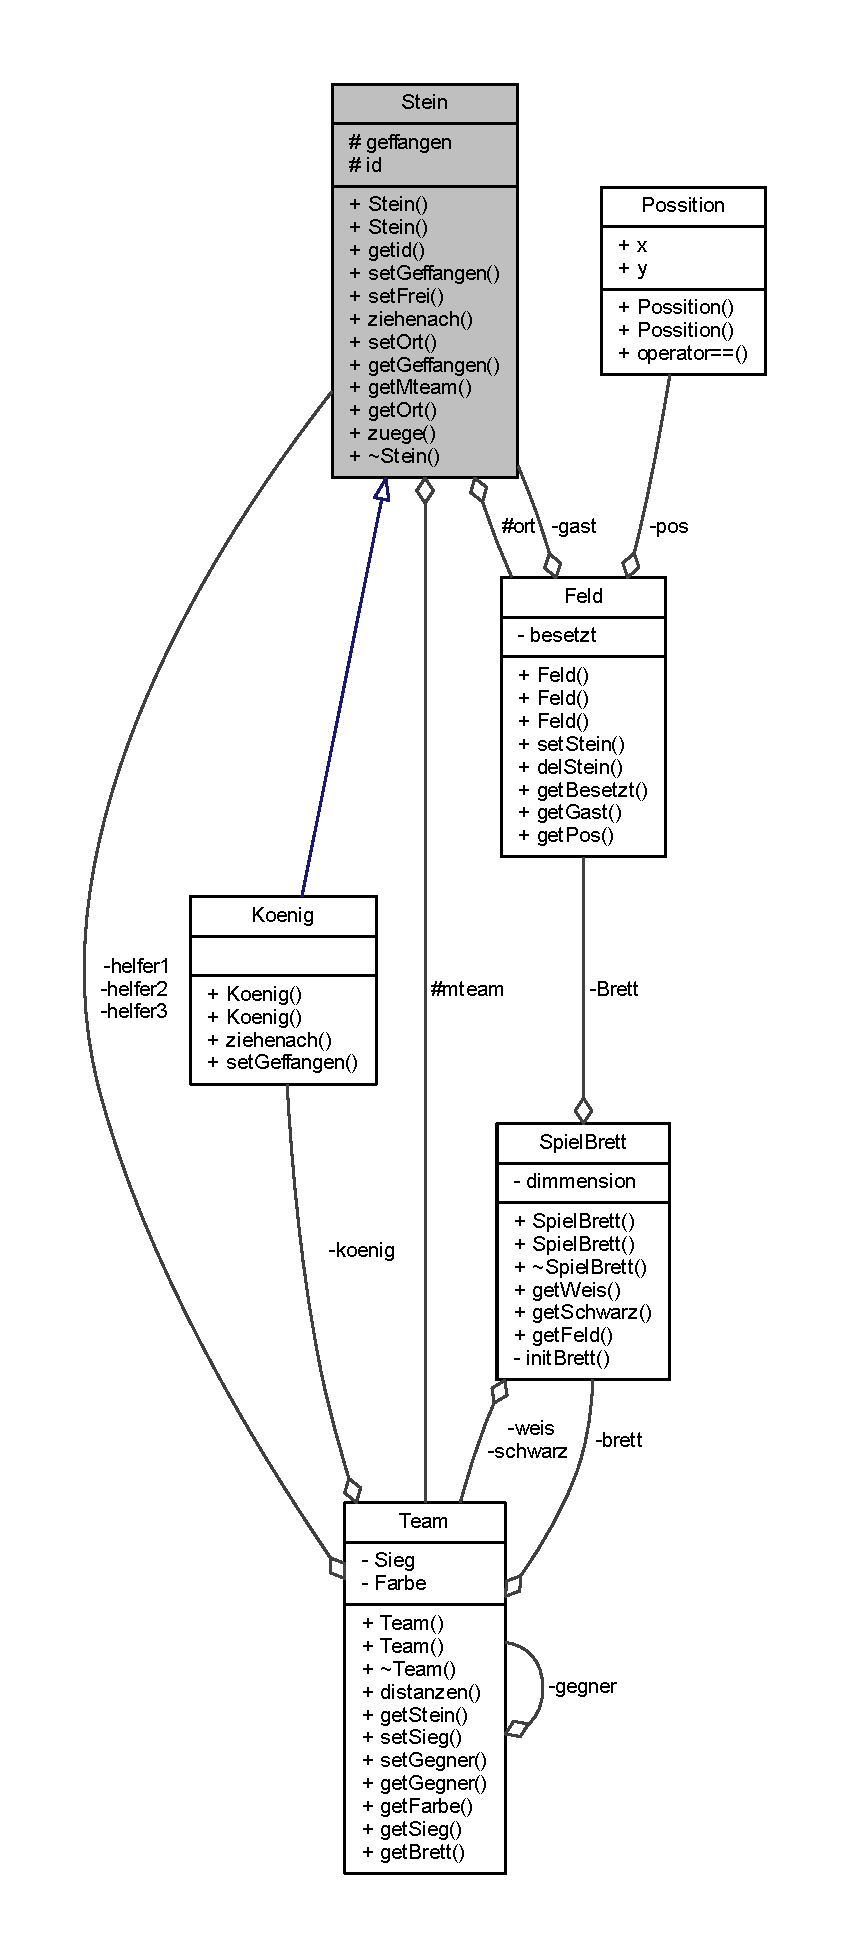
\includegraphics[height=550pt]{class_stein__coll__graph}
\end{center}
\end{figure}
\subsection*{Öffentliche Methoden}
\begin{DoxyCompactItemize}
\item 
\hyperlink{class_stein_a04fd5b2d635673ebf25d1c1cdac886c2}{Stein} ()
\item 
\hyperlink{class_stein_a4296de20f474a5186e1830025600b8bd}{Stein} (int \hyperlink{class_stein_ab8a179db9a227d710ce7d236ecae37ee}{id}, \hyperlink{class_feld}{Feld} $\ast$startplatz, \hyperlink{class_team}{Team} $\ast$mt)
\item 
int \hyperlink{class_stein_a2076f66967b65fcb8e551e9522222a95}{getid} () const 
\item 
virtual void \hyperlink{class_stein_a8a98cf8c96426bf5164c6eb41b03154b}{set\+Geffangen} ()
\item 
void \hyperlink{class_stein_a7136341c45149bfb929134b87f180a5b}{set\+Frei} ()
\item 
virtual bool \hyperlink{class_stein_afdac18155661536e25eda360038c1ca7}{ziehenach} (\hyperlink{class_feld}{Feld} $\ast$ziehl)
\item 
void \hyperlink{class_stein_a84a9276f99fd15f2f16d31c5c33cc66c}{set\+Ort} (\hyperlink{class_feld}{Feld} $\ast$o)
\item 
bool \hyperlink{class_stein_a00dce1ad2cade0f5570d3e5c3b835a5b}{get\+Geffangen} ()
\item 
\hyperlink{class_team}{Team} $\ast$ \hyperlink{class_stein_aa8e6142169b14b20350ffb2e0fa526ce}{get\+Mteam} ()
\item 
\hyperlink{class_feld}{Feld} $\ast$ \hyperlink{class_stein_af1c9430ba1a60572e73d9ed16199e185}{get\+Ort} ()
\item 
std\+::vector$<$ \hyperlink{class_feld}{Feld} $\ast$ $>$ \hyperlink{class_stein_a788ece6ca232c408243620cfbc943382}{zuege} ()
\item 
virtual \hyperlink{class_stein_aeebc529dd953c23c35a3ad8f8f78981d}{$\sim$\+Stein} ()=default
\end{DoxyCompactItemize}
\subsection*{Geschützte Attribute}
\begin{DoxyCompactItemize}
\item 
bool \hyperlink{class_stein_a4151b35edce6df36a415536c9fd0d247}{geffangen} =false
\item 
\hyperlink{class_feld}{Feld} $\ast$ \hyperlink{class_stein_aee940baa567743384754215cbdb5657d}{ort} =nullptr
\item 
\hyperlink{class_team}{Team} $\ast$ \hyperlink{class_stein_ae2b58e289026a8afaf8e22f8b9ad3d9c}{mteam} =nullptr
\item 
const int \hyperlink{class_stein_ab8a179db9a227d710ce7d236ecae37ee}{id}
\end{DoxyCompactItemize}


\subsection{Ausführliche Beschreibung}
class \hyperlink{class_stein}{Stein}

Jedes \hyperlink{class_team}{Team} besitzt drei Helfer. Sie können sich auf dem Spielfeld bewegen, festgesetzt (gefangen) werden, gegnerische Spielfiguren festsetzen, indem man sie ganz einfach auf das vom Gegner besetzte \hyperlink{class_feld}{Feld} schickt und in Verbindung mit dem teameigenen König können sie auch selber befreit werden, sollte der Gegner sie gefangen genommen haben. Jede Spielfigur und damit auch jeder Helfer, bekommt bei Spielbeginn einen Platz mittels Pointern zugewiesen. Die Spielfigur-\/\+I\+D und die Spielfeld-\/\+I\+D bestimmen also, welche Spielfigur von welchem \hyperlink{class_team}{Team} sich wo im \hyperlink{class_feld}{Feld} befindet. 

\subsection{Beschreibung der Konstruktoren und Destruktoren}
\hypertarget{class_stein_a04fd5b2d635673ebf25d1c1cdac886c2}{}\index{Stein@{Stein}!Stein@{Stein}}
\index{Stein@{Stein}!Stein@{Stein}}
\subsubsection[{Stein}]{\setlength{\rightskip}{0pt plus 5cm}Stein\+::\+Stein (
\begin{DoxyParamCaption}
{}
\end{DoxyParamCaption}
)}\label{class_stein_a04fd5b2d635673ebf25d1c1cdac886c2}
Konstruktor \hypertarget{class_stein_a4296de20f474a5186e1830025600b8bd}{}\index{Stein@{Stein}!Stein@{Stein}}
\index{Stein@{Stein}!Stein@{Stein}}
\subsubsection[{Stein}]{\setlength{\rightskip}{0pt plus 5cm}Stein\+::\+Stein (
\begin{DoxyParamCaption}
\item[{int}]{id, }
\item[{{\bf Feld} $\ast$}]{startplatz, }
\item[{{\bf Team} $\ast$}]{mt}
\end{DoxyParamCaption}
)}\label{class_stein_a4296de20f474a5186e1830025600b8bd}


Hier ist ein Graph, der zeigt, was diese Funktion aufruft\+:\nopagebreak
\begin{figure}[H]
\begin{center}
\leavevmode
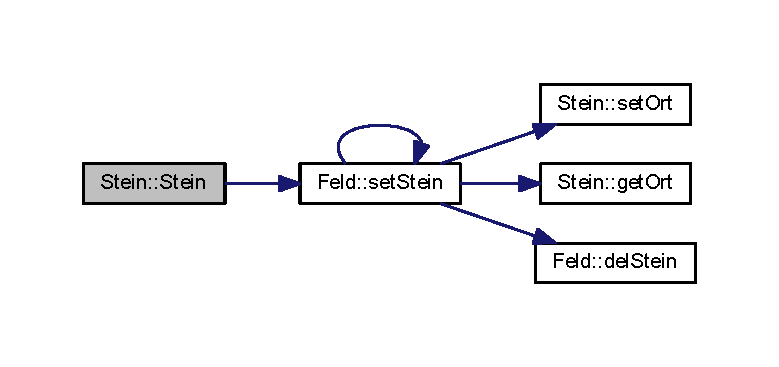
\includegraphics[width=350pt]{class_stein_a4296de20f474a5186e1830025600b8bd_cgraph}
\end{center}
\end{figure}


\hypertarget{class_stein_aeebc529dd953c23c35a3ad8f8f78981d}{}\index{Stein@{Stein}!````~Stein@{$\sim$\+Stein}}
\index{````~Stein@{$\sim$\+Stein}!Stein@{Stein}}
\subsubsection[{$\sim$\+Stein}]{\setlength{\rightskip}{0pt plus 5cm}virtual Stein\+::$\sim$\+Stein (
\begin{DoxyParamCaption}
{}
\end{DoxyParamCaption}
)\hspace{0.3cm}{\ttfamily [virtual]}, {\ttfamily [default]}}\label{class_stein_aeebc529dd953c23c35a3ad8f8f78981d}


\subsection{Dokumentation der Elementfunktionen}
\hypertarget{class_stein_a00dce1ad2cade0f5570d3e5c3b835a5b}{}\index{Stein@{Stein}!get\+Geffangen@{get\+Geffangen}}
\index{get\+Geffangen@{get\+Geffangen}!Stein@{Stein}}
\subsubsection[{get\+Geffangen}]{\setlength{\rightskip}{0pt plus 5cm}bool Stein\+::get\+Geffangen (
\begin{DoxyParamCaption}
{}
\end{DoxyParamCaption}
)}\label{class_stein_a00dce1ad2cade0f5570d3e5c3b835a5b}
\hyperlink{class_stein_a00dce1ad2cade0f5570d3e5c3b835a5b}{get\+Geffangen()} Die Funktion beschreibt, ob der \hyperlink{class_stein}{Stein} gefangen ist oder nicht. \begin{DoxyReturn}{Rückgabe}
the value of gefangen 
\end{DoxyReturn}
\hypertarget{class_stein_a2076f66967b65fcb8e551e9522222a95}{}\index{Stein@{Stein}!getid@{getid}}
\index{getid@{getid}!Stein@{Stein}}
\subsubsection[{getid}]{\setlength{\rightskip}{0pt plus 5cm}int Stein\+::getid (
\begin{DoxyParamCaption}
{}
\end{DoxyParamCaption}
) const}\label{class_stein_a2076f66967b65fcb8e551e9522222a95}
\hyperlink{class_stein_a2076f66967b65fcb8e551e9522222a95}{getid()} \hyperlink{class_stein_a2076f66967b65fcb8e551e9522222a95}{getid()} Diese Funktion sagt aus, ob es sich hierbei um weiß oder schwarz handelt. \begin{DoxyReturn}{Rückgabe}
id der Instanz 
\end{DoxyReturn}
\hypertarget{class_stein_aa8e6142169b14b20350ffb2e0fa526ce}{}\index{Stein@{Stein}!get\+Mteam@{get\+Mteam}}
\index{get\+Mteam@{get\+Mteam}!Stein@{Stein}}
\subsubsection[{get\+Mteam}]{\setlength{\rightskip}{0pt plus 5cm}{\bf Team} $\ast$ Stein\+::get\+Mteam (
\begin{DoxyParamCaption}
{}
\end{DoxyParamCaption}
)}\label{class_stein_aa8e6142169b14b20350ffb2e0fa526ce}
\hypertarget{class_stein_af1c9430ba1a60572e73d9ed16199e185}{}\index{Stein@{Stein}!get\+Ort@{get\+Ort}}
\index{get\+Ort@{get\+Ort}!Stein@{Stein}}
\subsubsection[{get\+Ort}]{\setlength{\rightskip}{0pt plus 5cm}{\bf Feld} $\ast$ Stein\+::get\+Ort (
\begin{DoxyParamCaption}
{}
\end{DoxyParamCaption}
)}\label{class_stein_af1c9430ba1a60572e73d9ed16199e185}
\hypertarget{class_stein_a7136341c45149bfb929134b87f180a5b}{}\index{Stein@{Stein}!set\+Frei@{set\+Frei}}
\index{set\+Frei@{set\+Frei}!Stein@{Stein}}
\subsubsection[{set\+Frei}]{\setlength{\rightskip}{0pt plus 5cm}void Stein\+::set\+Frei (
\begin{DoxyParamCaption}
{}
\end{DoxyParamCaption}
)}\label{class_stein_a7136341c45149bfb929134b87f180a5b}
\hyperlink{class_stein_a7136341c45149bfb929134b87f180a5b}{set\+Frei()} Setzt den \hyperlink{class_stein}{Stein} frei Setzt gefangen -\/$>$ false \hypertarget{class_stein_a8a98cf8c96426bf5164c6eb41b03154b}{}\index{Stein@{Stein}!set\+Geffangen@{set\+Geffangen}}
\index{set\+Geffangen@{set\+Geffangen}!Stein@{Stein}}
\subsubsection[{set\+Geffangen}]{\setlength{\rightskip}{0pt plus 5cm}void Stein\+::set\+Geffangen (
\begin{DoxyParamCaption}
{}
\end{DoxyParamCaption}
)\hspace{0.3cm}{\ttfamily [virtual]}}\label{class_stein_a8a98cf8c96426bf5164c6eb41b03154b}
set\+Gefangen() Setzt den \hyperlink{class_stein}{Stein} gefangen. gefangen -\/$>$ true 

Erneute Implementation in \hyperlink{class_koenig_a66d3242a51e934cc35bb8adabdba8a4a}{Koenig}.

\hypertarget{class_stein_a84a9276f99fd15f2f16d31c5c33cc66c}{}\index{Stein@{Stein}!set\+Ort@{set\+Ort}}
\index{set\+Ort@{set\+Ort}!Stein@{Stein}}
\subsubsection[{set\+Ort}]{\setlength{\rightskip}{0pt plus 5cm}void Stein\+::set\+Ort (
\begin{DoxyParamCaption}
\item[{{\bf Feld} $\ast$}]{o}
\end{DoxyParamCaption}
)}\label{class_stein_a84a9276f99fd15f2f16d31c5c33cc66c}
\hypertarget{class_stein_afdac18155661536e25eda360038c1ca7}{}\index{Stein@{Stein}!ziehenach@{ziehenach}}
\index{ziehenach@{ziehenach}!Stein@{Stein}}
\subsubsection[{ziehenach}]{\setlength{\rightskip}{0pt plus 5cm}bool Stein\+::ziehenach (
\begin{DoxyParamCaption}
\item[{{\bf Feld} $\ast$}]{ziehl}
\end{DoxyParamCaption}
)\hspace{0.3cm}{\ttfamily [virtual]}}\label{class_stein_afdac18155661536e25eda360038c1ca7}
set\+Ort Rückt auf das übergebene \hyperlink{class_feld}{Feld}. 
\begin{DoxyParams}{Parameter}
{\em \mbox{[}\+Feld\mbox{]}} & gibt die neue Position an \\
\hline
\end{DoxyParams}


Erneute Implementation in \hyperlink{class_koenig_a6060e36b885b96aad97fa4c66646942f}{Koenig}.



Hier ist ein Graph, der zeigt, was diese Funktion aufruft\+:\nopagebreak
\begin{figure}[H]
\begin{center}
\leavevmode
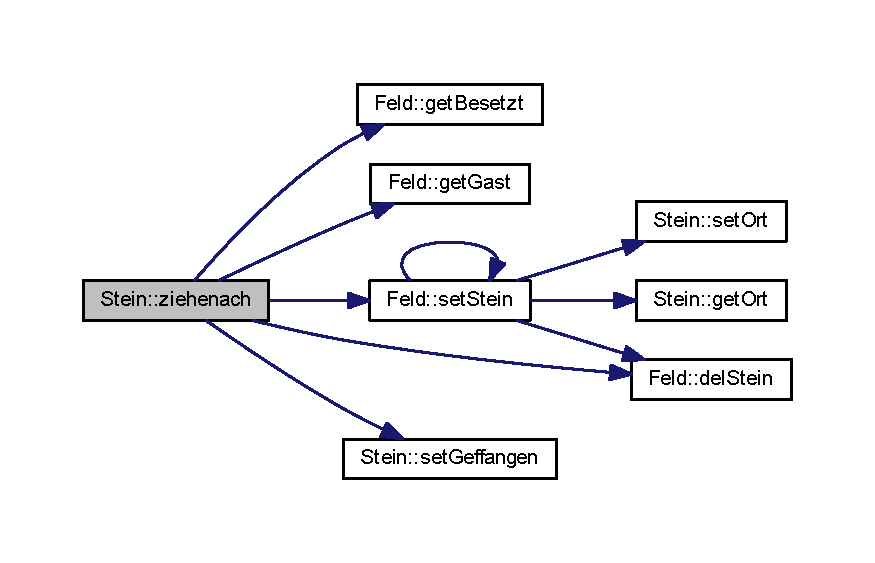
\includegraphics[width=350pt]{class_stein_afdac18155661536e25eda360038c1ca7_cgraph}
\end{center}
\end{figure}


\hypertarget{class_stein_a788ece6ca232c408243620cfbc943382}{}\index{Stein@{Stein}!zuege@{zuege}}
\index{zuege@{zuege}!Stein@{Stein}}
\subsubsection[{zuege}]{\setlength{\rightskip}{0pt plus 5cm}std\+::vector$<$ {\bf Feld} $\ast$ $>$ Stein\+::zuege (
\begin{DoxyParamCaption}
{}
\end{DoxyParamCaption}
)}\label{class_stein_a788ece6ca232c408243620cfbc943382}
\hyperlink{class_stein_a788ece6ca232c408243620cfbc943382}{zuege()} Die Funktion Zuege ermittelt alle möglichen Züge und gibt diese als Vector zurück. \begin{DoxyReturn}{Rückgabe}
\hyperlink{class_feld}{Feld} zue 
\end{DoxyReturn}


Hier ist ein Graph, der zeigt, was diese Funktion aufruft\+:\nopagebreak
\begin{figure}[H]
\begin{center}
\leavevmode
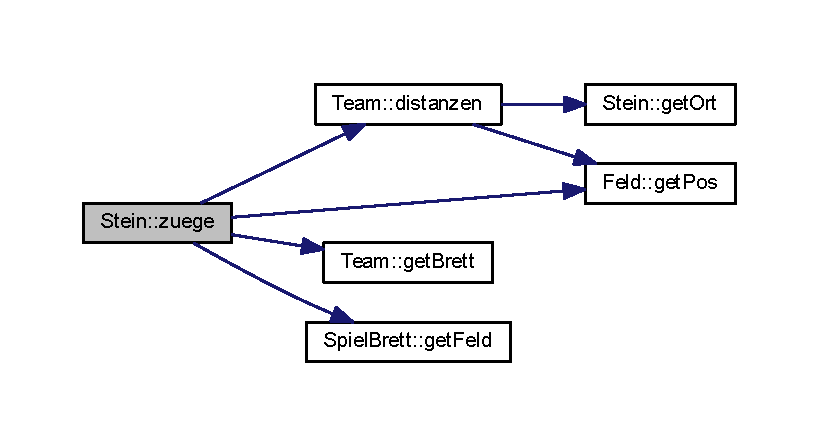
\includegraphics[width=350pt]{class_stein_a788ece6ca232c408243620cfbc943382_cgraph}
\end{center}
\end{figure}




\subsection{Dokumentation der Datenelemente}
\hypertarget{class_stein_a4151b35edce6df36a415536c9fd0d247}{}\index{Stein@{Stein}!geffangen@{geffangen}}
\index{geffangen@{geffangen}!Stein@{Stein}}
\subsubsection[{geffangen}]{\setlength{\rightskip}{0pt plus 5cm}bool Stein\+::geffangen =false\hspace{0.3cm}{\ttfamily [protected]}}\label{class_stein_a4151b35edce6df36a415536c9fd0d247}
\hypertarget{class_stein_ab8a179db9a227d710ce7d236ecae37ee}{}\index{Stein@{Stein}!id@{id}}
\index{id@{id}!Stein@{Stein}}
\subsubsection[{id}]{\setlength{\rightskip}{0pt plus 5cm}const int Stein\+::id\hspace{0.3cm}{\ttfamily [protected]}}\label{class_stein_ab8a179db9a227d710ce7d236ecae37ee}
\hypertarget{class_stein_ae2b58e289026a8afaf8e22f8b9ad3d9c}{}\index{Stein@{Stein}!mteam@{mteam}}
\index{mteam@{mteam}!Stein@{Stein}}
\subsubsection[{mteam}]{\setlength{\rightskip}{0pt plus 5cm}{\bf Team}$\ast$ Stein\+::mteam =nullptr\hspace{0.3cm}{\ttfamily [protected]}}\label{class_stein_ae2b58e289026a8afaf8e22f8b9ad3d9c}
\hypertarget{class_stein_aee940baa567743384754215cbdb5657d}{}\index{Stein@{Stein}!ort@{ort}}
\index{ort@{ort}!Stein@{Stein}}
\subsubsection[{ort}]{\setlength{\rightskip}{0pt plus 5cm}{\bf Feld}$\ast$ Stein\+::ort =nullptr\hspace{0.3cm}{\ttfamily [protected]}}\label{class_stein_aee940baa567743384754215cbdb5657d}


Die Dokumentation für diese Klasse wurde erzeugt aufgrund der Dateien\+:\begin{DoxyCompactItemize}
\item 
\hyperlink{_stein_8h}{Stein.\+h}\item 
\hyperlink{_stein_8cpp}{Stein.\+cpp}\end{DoxyCompactItemize}

\hypertarget{class_strategie}{}\section{Strategie Klassenreferenz}
\label{class_strategie}\index{Strategie@{Strategie}}


{\ttfamily \#include $<$Strategie.\+h$>$}



Klassendiagramm für Strategie\+:\nopagebreak
\begin{figure}[H]
\begin{center}
\leavevmode
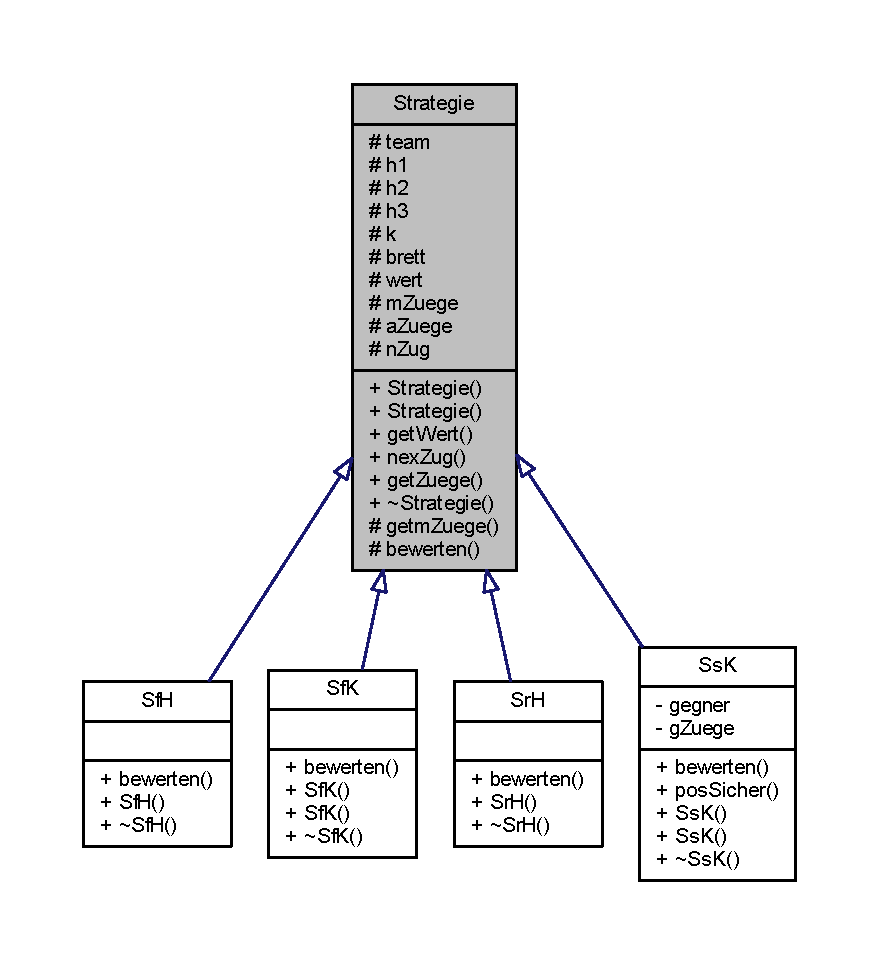
\includegraphics[width=350pt]{class_strategie__inherit__graph}
\end{center}
\end{figure}


Zusammengehörigkeiten von Strategie\+:\nopagebreak
\begin{figure}[H]
\begin{center}
\leavevmode
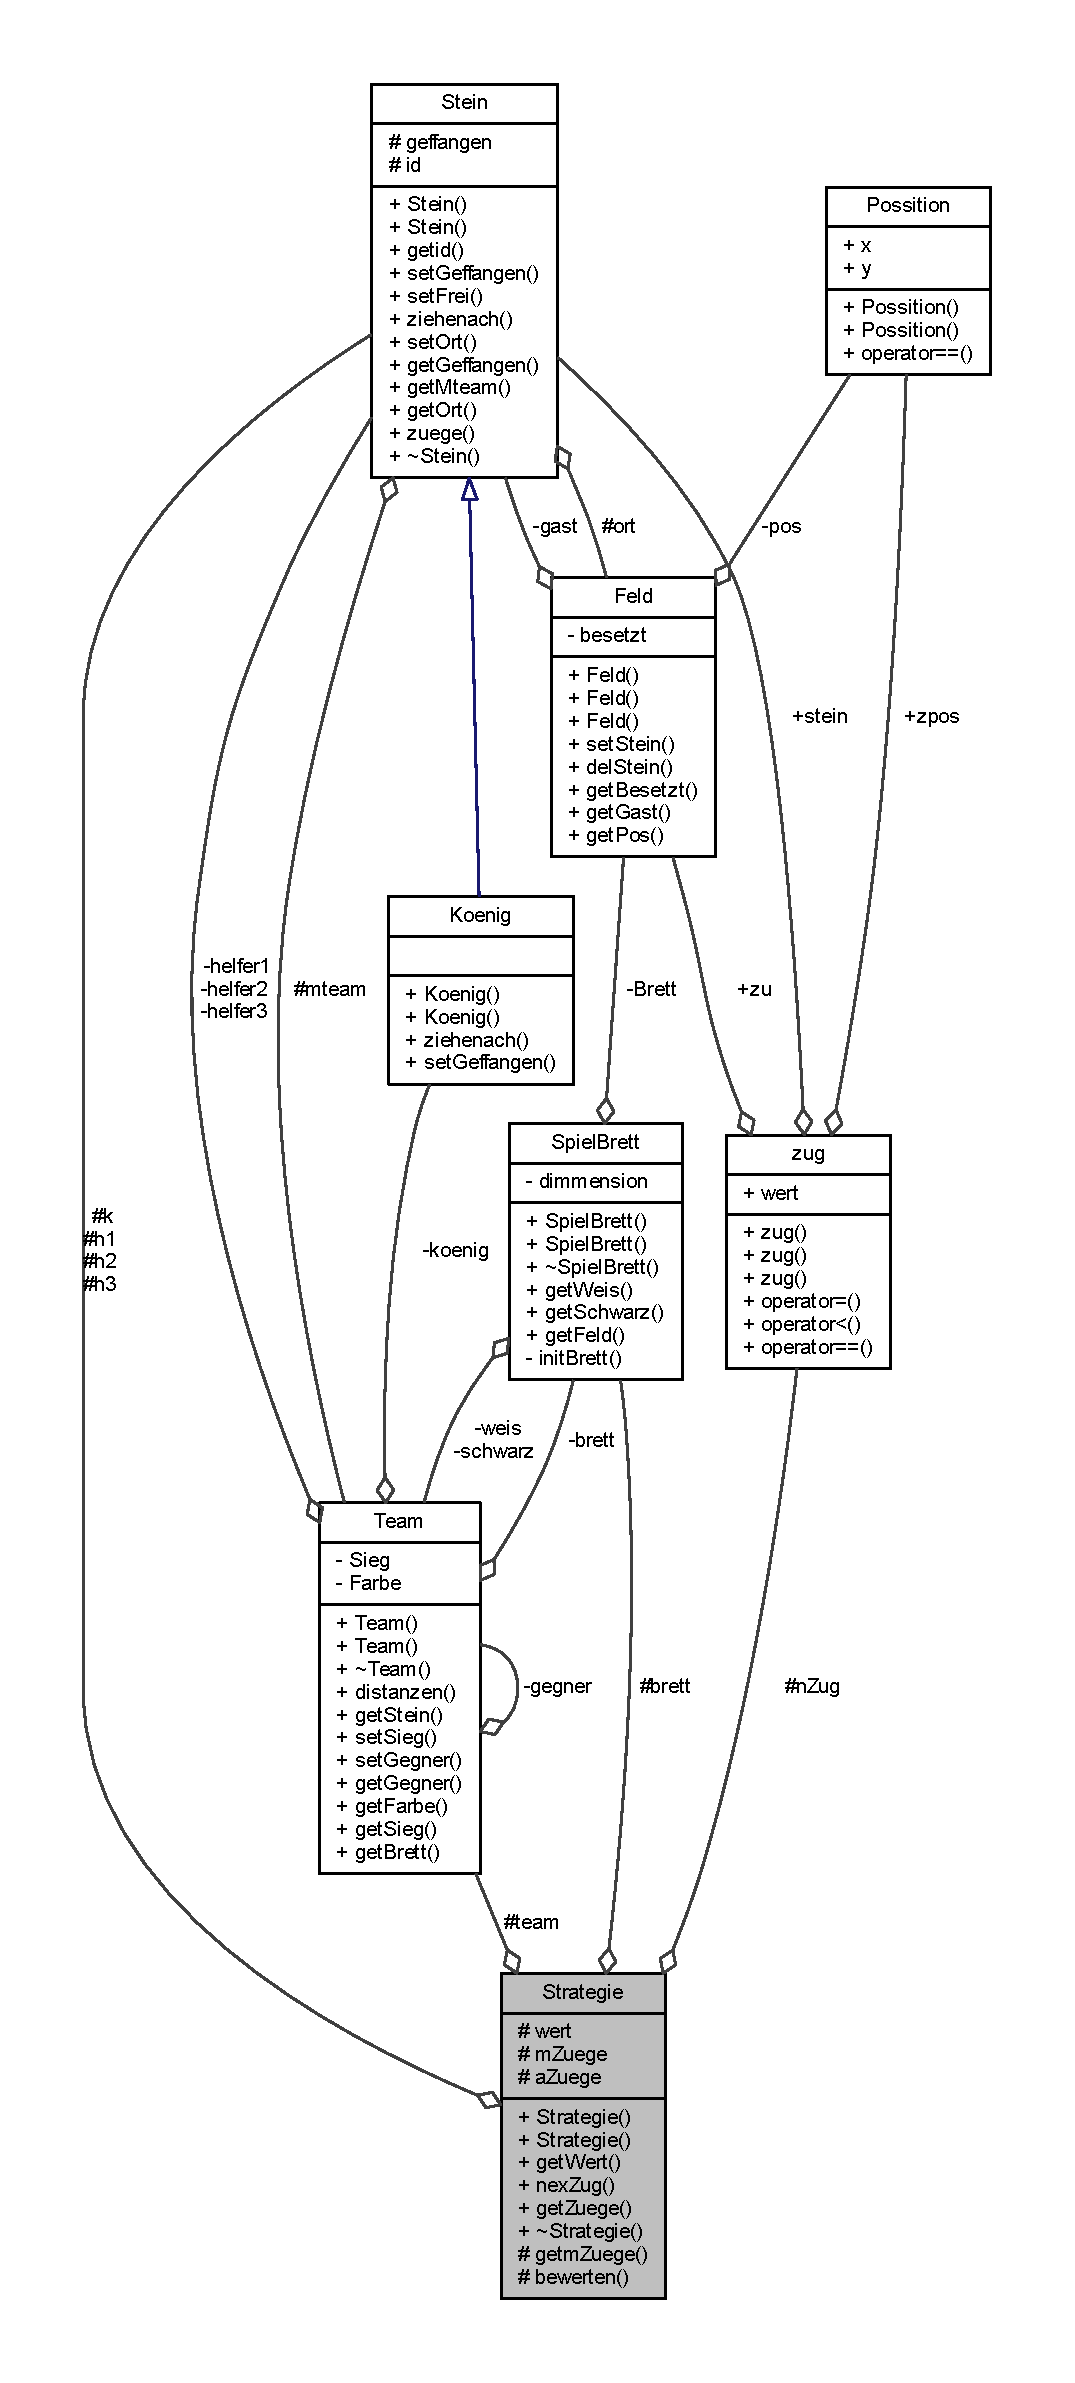
\includegraphics[height=550pt]{class_strategie__coll__graph}
\end{center}
\end{figure}
\subsection*{Öffentliche Methoden}
\begin{DoxyCompactItemize}
\item 
\hyperlink{class_strategie_a607fb1d583895e1e61905488e8836933}{Strategie} (\hyperlink{class_team}{Team} \&\hyperlink{class_strategie_a4f55e74f189ec8c6df88a57119fb3def}{team}, \hyperlink{class_spiel_brett}{Spiel\+Brett} \&b)
\item 
\hyperlink{class_strategie_a374010dd594a0977765d179377e76c12}{Strategie} ()
\item 
int \hyperlink{class_strategie_afeba2e4743f7cfe036115b92af4fc624}{get\+Wert} () const 
\item 
\hyperlink{structzug}{zug} \hyperlink{class_strategie_a106e1746778cc926fc7392c3224025b1}{nex\+Zug} ()
\item 
std\+::vector$<$ \hyperlink{structzug}{zug} $>$ \hyperlink{class_strategie_a4fd1fa322e0c44651cd72893c3ed5e9c}{get\+Zuege} () const 
\item 
virtual \hyperlink{class_strategie_a6eaa087b8a8f41d3e99ce7ed617d0432}{$\sim$\+Strategie} ()
\end{DoxyCompactItemize}
\subsection*{Geschützte Methoden}
\begin{DoxyCompactItemize}
\item 
void \hyperlink{class_strategie_a0766167436598f635562bcf8b3b10430}{getm\+Zuege} (std\+::vector$<$ \hyperlink{structzug}{zug} $>$ \&zuege)
\item 
virtual void \hyperlink{class_strategie_a6e11413c1c8e4ca8bd0bcac21be3c1bf}{bewerten} ()=0
\end{DoxyCompactItemize}
\subsection*{Geschützte Attribute}
\begin{DoxyCompactItemize}
\item 
\hyperlink{class_team}{Team} \& \hyperlink{class_strategie_a4f55e74f189ec8c6df88a57119fb3def}{team}
\item 
\hyperlink{class_stein}{Stein} \& \hyperlink{class_strategie_a0b64b5969f835653965957eab7f1f5a9}{h1}
\item 
\hyperlink{class_stein}{Stein} \& \hyperlink{class_strategie_a6721c42de183333c6f49fe9724b907ae}{h2}
\item 
\hyperlink{class_stein}{Stein} \& \hyperlink{class_strategie_a82f2549dabdf1afbe888405d1adfb9e6}{h3}
\item 
\hyperlink{class_stein}{Stein} \& \hyperlink{class_strategie_abbf970c05c0033ae9f5df3766316846c}{k}
\item 
\hyperlink{class_spiel_brett}{Spiel\+Brett} \& \hyperlink{class_strategie_a2a498380f5a837cd9e5afdd9b546ed46}{brett}
\item 
int \hyperlink{class_strategie_ad0b73259d206b7114d026f7c50074554}{wert}
\item 
std\+::vector$<$ \hyperlink{structzug}{zug} $>$ \hyperlink{class_strategie_a99c5724d40dc860fc30c17a449815aa5}{m\+Zuege}
\item 
std\+::vector$<$ \hyperlink{structzug}{zug} $>$ \hyperlink{class_strategie_a6d800c6d8636540d16b41d7abf8c9ad3}{a\+Zuege}
\item 
\hyperlink{structzug}{zug} \hyperlink{class_strategie_a3f2847acbd3cd961853f0eadb6c05daf}{n\+Zug}
\end{DoxyCompactItemize}


\subsection{Ausführliche Beschreibung}
class \hyperlink{class_strategie}{Strategie}

Abstrakte Klasse zur Erzeugung von speziellen Zug-\/\+Strategien.

Als Strategien sind jene Funktionen gemeint, welche neben der Bewegung im \hyperlink{class_feld}{Feld}, zusätzlich auch dafür sorgen, dass es zu einer Sieg/\+Niederlage Situation kommt. Sie stellen die Möglichkeiten dar, welche die Spielfiguren in den jeweiligen Momenten besitzen. Die Bewertung erfolgt in Echtzeit.

Wir programmierten 4 Strategien ein. Jede der 4 Strategien ist eine Vererbung dieser Klasse. 

\subsection{Beschreibung der Konstruktoren und Destruktoren}
\hypertarget{class_strategie_a607fb1d583895e1e61905488e8836933}{}\index{Strategie@{Strategie}!Strategie@{Strategie}}
\index{Strategie@{Strategie}!Strategie@{Strategie}}
\subsubsection[{Strategie}]{\setlength{\rightskip}{0pt plus 5cm}Strategie\+::\+Strategie (
\begin{DoxyParamCaption}
\item[{{\bf Team} \&}]{team, }
\item[{{\bf Spiel\+Brett} \&}]{b}
\end{DoxyParamCaption}
)}\label{class_strategie_a607fb1d583895e1e61905488e8836933}
\hypertarget{class_strategie_a374010dd594a0977765d179377e76c12}{}\index{Strategie@{Strategie}!Strategie@{Strategie}}
\index{Strategie@{Strategie}!Strategie@{Strategie}}
\subsubsection[{Strategie}]{\setlength{\rightskip}{0pt plus 5cm}Strategie\+::\+Strategie (
\begin{DoxyParamCaption}
{}
\end{DoxyParamCaption}
)}\label{class_strategie_a374010dd594a0977765d179377e76c12}
\hypertarget{class_strategie_a6eaa087b8a8f41d3e99ce7ed617d0432}{}\index{Strategie@{Strategie}!````~Strategie@{$\sim$\+Strategie}}
\index{````~Strategie@{$\sim$\+Strategie}!Strategie@{Strategie}}
\subsubsection[{$\sim$\+Strategie}]{\setlength{\rightskip}{0pt plus 5cm}Strategie\+::$\sim$\+Strategie (
\begin{DoxyParamCaption}
{}
\end{DoxyParamCaption}
)\hspace{0.3cm}{\ttfamily [virtual]}}\label{class_strategie_a6eaa087b8a8f41d3e99ce7ed617d0432}


\subsection{Dokumentation der Elementfunktionen}
\hypertarget{class_strategie_a6e11413c1c8e4ca8bd0bcac21be3c1bf}{}\index{Strategie@{Strategie}!bewerten@{bewerten}}
\index{bewerten@{bewerten}!Strategie@{Strategie}}
\subsubsection[{bewerten}]{\setlength{\rightskip}{0pt plus 5cm}void Strategie\+::bewerten (
\begin{DoxyParamCaption}
{}
\end{DoxyParamCaption}
)\hspace{0.3cm}{\ttfamily [protected]}, {\ttfamily [pure virtual]}}\label{class_strategie_a6e11413c1c8e4ca8bd0bcac21be3c1bf}


Implementiert in \hyperlink{class_sf_k_a54410f0aa0c2f76704a0eb181a5737f0}{Sf\+K}, \hyperlink{class_sf_h_a9790a3fab6619e16961568d735678d4f}{Sf\+H}, \hyperlink{class_ss_k_aac922686e66332aae431ec05d06937a0}{Ss\+K} und \hyperlink{class_sr_h_a55d77665881d6810fbde7d761ecbb02c}{Sr\+H}.

\hypertarget{class_strategie_a0766167436598f635562bcf8b3b10430}{}\index{Strategie@{Strategie}!getm\+Zuege@{getm\+Zuege}}
\index{getm\+Zuege@{getm\+Zuege}!Strategie@{Strategie}}
\subsubsection[{getm\+Zuege}]{\setlength{\rightskip}{0pt plus 5cm}void Strategie\+::getm\+Zuege (
\begin{DoxyParamCaption}
\item[{std\+::vector$<$ {\bf zug} $>$ \&}]{zuege}
\end{DoxyParamCaption}
)\hspace{0.3cm}{\ttfamily [protected]}}\label{class_strategie_a0766167436598f635562bcf8b3b10430}


Hier ist ein Graph, der zeigt, was diese Funktion aufruft\+:\nopagebreak
\begin{figure}[H]
\begin{center}
\leavevmode
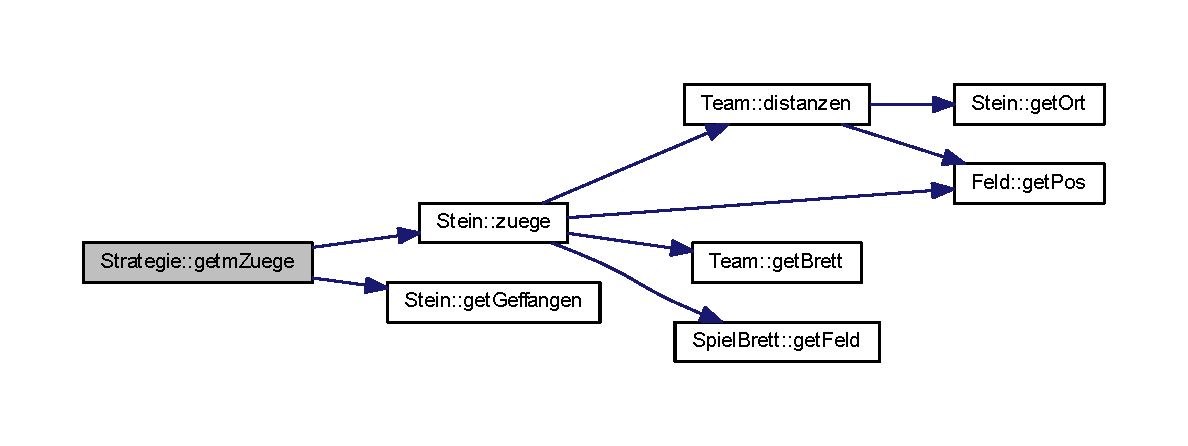
\includegraphics[width=350pt]{class_strategie_a0766167436598f635562bcf8b3b10430_cgraph}
\end{center}
\end{figure}


\hypertarget{class_strategie_afeba2e4743f7cfe036115b92af4fc624}{}\index{Strategie@{Strategie}!get\+Wert@{get\+Wert}}
\index{get\+Wert@{get\+Wert}!Strategie@{Strategie}}
\subsubsection[{get\+Wert}]{\setlength{\rightskip}{0pt plus 5cm}int Strategie\+::get\+Wert (
\begin{DoxyParamCaption}
{}
\end{DoxyParamCaption}
) const}\label{class_strategie_afeba2e4743f7cfe036115b92af4fc624}
\hypertarget{class_strategie_a4fd1fa322e0c44651cd72893c3ed5e9c}{}\index{Strategie@{Strategie}!get\+Zuege@{get\+Zuege}}
\index{get\+Zuege@{get\+Zuege}!Strategie@{Strategie}}
\subsubsection[{get\+Zuege}]{\setlength{\rightskip}{0pt plus 5cm}std\+::vector$<$ {\bf zug} $>$ Strategie\+::get\+Zuege (
\begin{DoxyParamCaption}
{}
\end{DoxyParamCaption}
) const}\label{class_strategie_a4fd1fa322e0c44651cd72893c3ed5e9c}
\hypertarget{class_strategie_a106e1746778cc926fc7392c3224025b1}{}\index{Strategie@{Strategie}!nex\+Zug@{nex\+Zug}}
\index{nex\+Zug@{nex\+Zug}!Strategie@{Strategie}}
\subsubsection[{nex\+Zug}]{\setlength{\rightskip}{0pt plus 5cm}{\bf zug} Strategie\+::nex\+Zug (
\begin{DoxyParamCaption}
{}
\end{DoxyParamCaption}
)}\label{class_strategie_a106e1746778cc926fc7392c3224025b1}


Hier ist ein Graph, der zeigt, was diese Funktion aufruft\+:\nopagebreak
\begin{figure}[H]
\begin{center}
\leavevmode
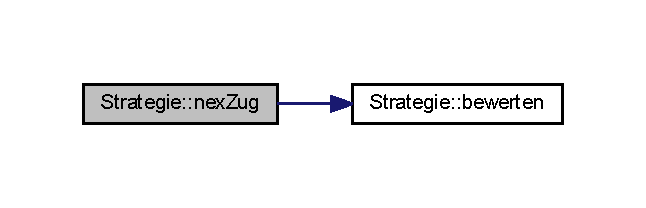
\includegraphics[width=310pt]{class_strategie_a106e1746778cc926fc7392c3224025b1_cgraph}
\end{center}
\end{figure}




\subsection{Dokumentation der Datenelemente}
\hypertarget{class_strategie_a6d800c6d8636540d16b41d7abf8c9ad3}{}\index{Strategie@{Strategie}!a\+Zuege@{a\+Zuege}}
\index{a\+Zuege@{a\+Zuege}!Strategie@{Strategie}}
\subsubsection[{a\+Zuege}]{\setlength{\rightskip}{0pt plus 5cm}std\+::vector$<${\bf zug}$>$ Strategie\+::a\+Zuege\hspace{0.3cm}{\ttfamily [protected]}}\label{class_strategie_a6d800c6d8636540d16b41d7abf8c9ad3}
\hypertarget{class_strategie_a2a498380f5a837cd9e5afdd9b546ed46}{}\index{Strategie@{Strategie}!brett@{brett}}
\index{brett@{brett}!Strategie@{Strategie}}
\subsubsection[{brett}]{\setlength{\rightskip}{0pt plus 5cm}{\bf Spiel\+Brett}\& Strategie\+::brett\hspace{0.3cm}{\ttfamily [protected]}}\label{class_strategie_a2a498380f5a837cd9e5afdd9b546ed46}
\hypertarget{class_strategie_a0b64b5969f835653965957eab7f1f5a9}{}\index{Strategie@{Strategie}!h1@{h1}}
\index{h1@{h1}!Strategie@{Strategie}}
\subsubsection[{h1}]{\setlength{\rightskip}{0pt plus 5cm}{\bf Stein}\& Strategie\+::h1\hspace{0.3cm}{\ttfamily [protected]}}\label{class_strategie_a0b64b5969f835653965957eab7f1f5a9}
\hypertarget{class_strategie_a6721c42de183333c6f49fe9724b907ae}{}\index{Strategie@{Strategie}!h2@{h2}}
\index{h2@{h2}!Strategie@{Strategie}}
\subsubsection[{h2}]{\setlength{\rightskip}{0pt plus 5cm}{\bf Stein} \& Strategie\+::h2\hspace{0.3cm}{\ttfamily [protected]}}\label{class_strategie_a6721c42de183333c6f49fe9724b907ae}
\hypertarget{class_strategie_a82f2549dabdf1afbe888405d1adfb9e6}{}\index{Strategie@{Strategie}!h3@{h3}}
\index{h3@{h3}!Strategie@{Strategie}}
\subsubsection[{h3}]{\setlength{\rightskip}{0pt plus 5cm}{\bf Stein} \& Strategie\+::h3\hspace{0.3cm}{\ttfamily [protected]}}\label{class_strategie_a82f2549dabdf1afbe888405d1adfb9e6}
\hypertarget{class_strategie_abbf970c05c0033ae9f5df3766316846c}{}\index{Strategie@{Strategie}!k@{k}}
\index{k@{k}!Strategie@{Strategie}}
\subsubsection[{k}]{\setlength{\rightskip}{0pt plus 5cm}{\bf Stein} \& Strategie\+::k\hspace{0.3cm}{\ttfamily [protected]}}\label{class_strategie_abbf970c05c0033ae9f5df3766316846c}
\hypertarget{class_strategie_a99c5724d40dc860fc30c17a449815aa5}{}\index{Strategie@{Strategie}!m\+Zuege@{m\+Zuege}}
\index{m\+Zuege@{m\+Zuege}!Strategie@{Strategie}}
\subsubsection[{m\+Zuege}]{\setlength{\rightskip}{0pt plus 5cm}std\+::vector$<${\bf zug}$>$ Strategie\+::m\+Zuege\hspace{0.3cm}{\ttfamily [protected]}}\label{class_strategie_a99c5724d40dc860fc30c17a449815aa5}
\hypertarget{class_strategie_a3f2847acbd3cd961853f0eadb6c05daf}{}\index{Strategie@{Strategie}!n\+Zug@{n\+Zug}}
\index{n\+Zug@{n\+Zug}!Strategie@{Strategie}}
\subsubsection[{n\+Zug}]{\setlength{\rightskip}{0pt plus 5cm}{\bf zug} Strategie\+::n\+Zug\hspace{0.3cm}{\ttfamily [protected]}}\label{class_strategie_a3f2847acbd3cd961853f0eadb6c05daf}
\hypertarget{class_strategie_a4f55e74f189ec8c6df88a57119fb3def}{}\index{Strategie@{Strategie}!team@{team}}
\index{team@{team}!Strategie@{Strategie}}
\subsubsection[{team}]{\setlength{\rightskip}{0pt plus 5cm}{\bf Team}\& Strategie\+::team\hspace{0.3cm}{\ttfamily [protected]}}\label{class_strategie_a4f55e74f189ec8c6df88a57119fb3def}
\hypertarget{class_strategie_ad0b73259d206b7114d026f7c50074554}{}\index{Strategie@{Strategie}!wert@{wert}}
\index{wert@{wert}!Strategie@{Strategie}}
\subsubsection[{wert}]{\setlength{\rightskip}{0pt plus 5cm}int Strategie\+::wert\hspace{0.3cm}{\ttfamily [protected]}}\label{class_strategie_ad0b73259d206b7114d026f7c50074554}


Die Dokumentation für diese Klasse wurde erzeugt aufgrund der Dateien\+:\begin{DoxyCompactItemize}
\item 
\hyperlink{_strategie_8h}{Strategie.\+h}\item 
\hyperlink{_strategie_8cpp}{Strategie.\+cpp}\end{DoxyCompactItemize}

\hypertarget{class_team}{}\section{Team Klassenreferenz}
\label{class_team}\index{Team@{Team}}


{\ttfamily \#include $<$Team.\+h$>$}



Zusammengehörigkeiten von Team\+:\nopagebreak
\begin{figure}[H]
\begin{center}
\leavevmode
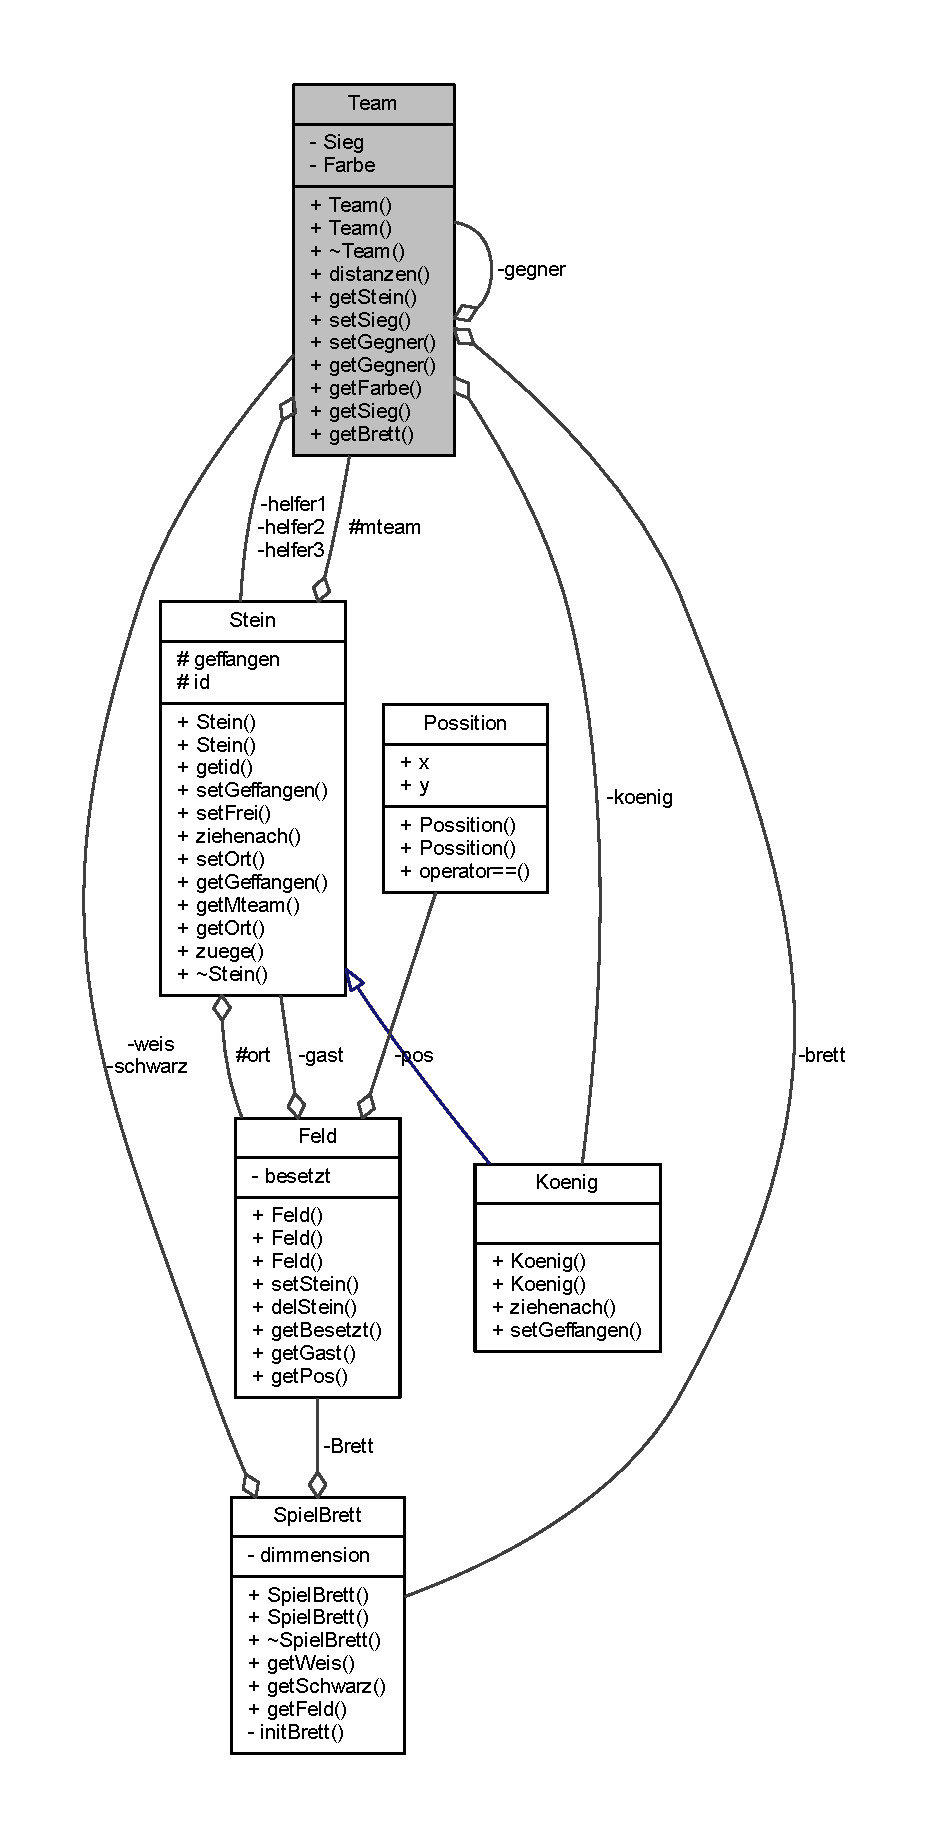
\includegraphics[height=550pt]{class_team__coll__graph}
\end{center}
\end{figure}
\subsection*{Öffentliche Methoden}
\begin{DoxyCompactItemize}
\item 
\hyperlink{class_team_ac246630434b2154b18d7538f3886f89d}{Team} (\hyperlink{class_spiel_brett}{Spiel\+Brett} $\ast$br, bool f, \hyperlink{class_feld}{Feld} $\ast$s1, \hyperlink{class_feld}{Feld} $\ast$s2, \hyperlink{class_feld}{Feld} $\ast$s3, \hyperlink{class_feld}{Feld} $\ast$k, \hyperlink{class_team}{Team} $\ast$g)
\item 
\hyperlink{class_team_af4b0ef286d67546ce8208aeceb4f576a}{Team} ()=default
\item 
virtual \hyperlink{class_team_ab4218fddd612d52bab47bec4feeb49de}{$\sim$\+Team} ()
\item 
void \hyperlink{class_team_aca8bdbcf6d3fd6e4efbe84fc158089b1}{distanzen} (const \hyperlink{class_stein}{Stein} \&anfrage, int $\ast$arr)
\item 
\hyperlink{class_stein}{Stein} \& \hyperlink{class_team_a458bc7ccfe8325b848723774a9564729}{get\+Stein} (int id) const 
\item 
void \hyperlink{class_team_a118a601e0db3871796a6c5be8ef7883d}{set\+Sieg} (bool new\+\_\+var)
\item 
void \hyperlink{class_team_a57428fa9c4911a089cd317e71f2018ab}{set\+Gegner} (\hyperlink{class_team}{Team} $\ast$new\+\_\+var)
\item 
\hyperlink{class_team}{Team} $\ast$ \hyperlink{class_team_a4342344f18da4e843ff8bf08525628ec}{get\+Gegner} () const 
\item 
bool \hyperlink{class_team_adabf037f25d619ba30f6d19a9fd5c888}{get\+Farbe} () const 
\item 
bool \hyperlink{class_team_a8d92a4f530838898bb9ca43a7da3ff8d}{get\+Sieg} ()
\item 
\hyperlink{class_spiel_brett}{Spiel\+Brett} $\ast$ \hyperlink{class_team_abd4d61dc0590e55c906f22bfd49b4eb7}{get\+Brett} () const 
\end{DoxyCompactItemize}
\subsection*{Private Attribute}
\begin{DoxyCompactItemize}
\item 
\hyperlink{class_stein}{Stein} $\ast$ \hyperlink{class_team_a567566ff8b74878120070386105bb60d}{helfer1} =nullptr
\item 
\hyperlink{class_stein}{Stein} $\ast$ \hyperlink{class_team_a9df764cfcf97e0ca9f386a91da041f1f}{helfer2} =nullptr
\item 
\hyperlink{class_stein}{Stein} $\ast$ \hyperlink{class_team_a5d3c196e4039c8e4666fcd0156f3129b}{helfer3} =nullptr
\item 
\hyperlink{class_koenig}{Koenig} $\ast$ \hyperlink{class_team_a7e8d3c991b52c5bb72ddeaf2a4cec935}{koenig} =nullptr
\item 
bool \hyperlink{class_team_af4db822bc0edd1ff703f3c792b4df99e}{Sieg} =false
\item 
\hyperlink{class_team}{Team} $\ast$ \hyperlink{class_team_ac5014169ca8a0a48b4d2aeac44e693dd}{gegner} =nullptr
\item 
\hyperlink{class_spiel_brett}{Spiel\+Brett} $\ast$ \hyperlink{class_team_a11297253f6cd542d16cadda671e858fc}{brett} =nullptr
\item 
bool \hyperlink{class_team_a8177ac0df0beef8c2489401000be6868}{Farbe} =false
\end{DoxyCompactItemize}


\subsection{Ausführliche Beschreibung}
class \hyperlink{class_team}{Team} 

\subsection{Beschreibung der Konstruktoren und Destruktoren}
\hypertarget{class_team_ac246630434b2154b18d7538f3886f89d}{}\index{Team@{Team}!Team@{Team}}
\index{Team@{Team}!Team@{Team}}
\subsubsection[{Team}]{\setlength{\rightskip}{0pt plus 5cm}Team\+::\+Team (
\begin{DoxyParamCaption}
\item[{{\bf Spiel\+Brett} $\ast$}]{br, }
\item[{bool}]{f, }
\item[{{\bf Feld} $\ast$}]{s1, }
\item[{{\bf Feld} $\ast$}]{s2, }
\item[{{\bf Feld} $\ast$}]{s3, }
\item[{{\bf Feld} $\ast$}]{k, }
\item[{{\bf Team} $\ast$}]{g = {\ttfamily nullptr}}
\end{DoxyParamCaption}
)}\label{class_team_ac246630434b2154b18d7538f3886f89d}
Erzeugt \hyperlink{class_team}{Team}. \hypertarget{class_team_af4b0ef286d67546ce8208aeceb4f576a}{}\index{Team@{Team}!Team@{Team}}
\index{Team@{Team}!Team@{Team}}
\subsubsection[{Team}]{\setlength{\rightskip}{0pt plus 5cm}Team\+::\+Team (
\begin{DoxyParamCaption}
{}
\end{DoxyParamCaption}
)\hspace{0.3cm}{\ttfamily [default]}}\label{class_team_af4b0ef286d67546ce8208aeceb4f576a}
\hypertarget{class_team_ab4218fddd612d52bab47bec4feeb49de}{}\index{Team@{Team}!````~Team@{$\sim$\+Team}}
\index{````~Team@{$\sim$\+Team}!Team@{Team}}
\subsubsection[{$\sim$\+Team}]{\setlength{\rightskip}{0pt plus 5cm}Team\+::$\sim$\+Team (
\begin{DoxyParamCaption}
{}
\end{DoxyParamCaption}
)\hspace{0.3cm}{\ttfamily [virtual]}}\label{class_team_ab4218fddd612d52bab47bec4feeb49de}


\subsection{Dokumentation der Elementfunktionen}
\hypertarget{class_team_aca8bdbcf6d3fd6e4efbe84fc158089b1}{}\index{Team@{Team}!distanzen@{distanzen}}
\index{distanzen@{distanzen}!Team@{Team}}
\subsubsection[{distanzen}]{\setlength{\rightskip}{0pt plus 5cm}void Team\+::distanzen (
\begin{DoxyParamCaption}
\item[{const {\bf Stein} \&}]{anfrage, }
\item[{int $\ast$}]{arr}
\end{DoxyParamCaption}
)}\label{class_team_aca8bdbcf6d3fd6e4efbe84fc158089b1}
\hyperlink{class_team_aca8bdbcf6d3fd6e4efbe84fc158089b1}{distanzen()} Trägt x und y Distanzen der \char`\"{}\+Anderen\char`\"{} Steine in einem Array ein. Array muss 6 Felder besitzen und vom Typ Integer sein.


\begin{DoxyParams}[1]{Parameter}
\mbox{\tt in}  & {\em \&anfrage} & \+: \hyperlink{class_stein}{Stein}, \mbox{[}out\mbox{]} $\ast$arr \+: int array\mbox{[}6\mbox{]}\\
\hline
\end{DoxyParams}
\begin{DoxyReturn}{Rückgabe}
unsigned short 
\end{DoxyReturn}

\begin{DoxyParams}{Parameter}
{\em anfrage} & \\
\hline
\end{DoxyParams}


Hier ist ein Graph, der zeigt, was diese Funktion aufruft\+:\nopagebreak
\begin{figure}[H]
\begin{center}
\leavevmode
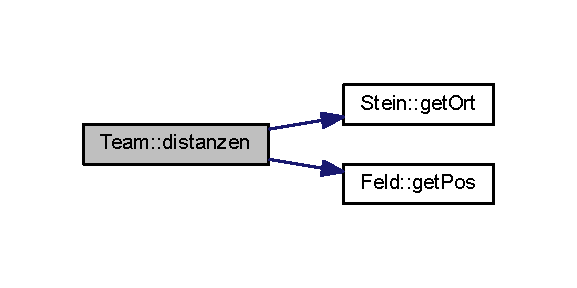
\includegraphics[width=277pt]{class_team_aca8bdbcf6d3fd6e4efbe84fc158089b1_cgraph}
\end{center}
\end{figure}


\hypertarget{class_team_abd4d61dc0590e55c906f22bfd49b4eb7}{}\index{Team@{Team}!get\+Brett@{get\+Brett}}
\index{get\+Brett@{get\+Brett}!Team@{Team}}
\subsubsection[{get\+Brett}]{\setlength{\rightskip}{0pt plus 5cm}{\bf Spiel\+Brett} $\ast$ Team\+::get\+Brett (
\begin{DoxyParamCaption}
{}
\end{DoxyParamCaption}
) const}\label{class_team_abd4d61dc0590e55c906f22bfd49b4eb7}
\hypertarget{class_team_adabf037f25d619ba30f6d19a9fd5c888}{}\index{Team@{Team}!get\+Farbe@{get\+Farbe}}
\index{get\+Farbe@{get\+Farbe}!Team@{Team}}
\subsubsection[{get\+Farbe}]{\setlength{\rightskip}{0pt plus 5cm}bool Team\+::get\+Farbe (
\begin{DoxyParamCaption}
{}
\end{DoxyParamCaption}
) const}\label{class_team_adabf037f25d619ba30f6d19a9fd5c888}
\hypertarget{class_team_a4342344f18da4e843ff8bf08525628ec}{}\index{Team@{Team}!get\+Gegner@{get\+Gegner}}
\index{get\+Gegner@{get\+Gegner}!Team@{Team}}
\subsubsection[{get\+Gegner}]{\setlength{\rightskip}{0pt plus 5cm}{\bf Team} $\ast$ Team\+::get\+Gegner (
\begin{DoxyParamCaption}
{}
\end{DoxyParamCaption}
) const}\label{class_team_a4342344f18da4e843ff8bf08525628ec}
Gibt Pointer auf Gegnerisches \hyperlink{class_team}{Team} aus. \hypertarget{class_team_a8d92a4f530838898bb9ca43a7da3ff8d}{}\index{Team@{Team}!get\+Sieg@{get\+Sieg}}
\index{get\+Sieg@{get\+Sieg}!Team@{Team}}
\subsubsection[{get\+Sieg}]{\setlength{\rightskip}{0pt plus 5cm}bool Team\+::get\+Sieg (
\begin{DoxyParamCaption}
{}
\end{DoxyParamCaption}
)}\label{class_team_a8d92a4f530838898bb9ca43a7da3ff8d}
\hypertarget{class_team_a458bc7ccfe8325b848723774a9564729}{}\index{Team@{Team}!get\+Stein@{get\+Stein}}
\index{get\+Stein@{get\+Stein}!Team@{Team}}
\subsubsection[{get\+Stein}]{\setlength{\rightskip}{0pt plus 5cm}{\bf Stein} \& Team\+::get\+Stein (
\begin{DoxyParamCaption}
\item[{int}]{id}
\end{DoxyParamCaption}
) const}\label{class_team_a458bc7ccfe8325b848723774a9564729}
get\+Stein Gibt Referenz auf \hyperlink{class_stein}{Stein} mit übergebener I\+D zurück, bei falschen I\+DŽs wird Referenz auf \hyperlink{class_koenig}{Koenig} zurückgegeben. 1-\/3 -\/$>$ Helfer 4 -\/$>$ \hyperlink{class_koenig}{Koenig} 
\begin{DoxyParams}[1]{Parameter}
\mbox{\tt in}  & {\em id} & \+: int \\
\hline
\end{DoxyParams}
\begin{DoxyReturn}{Rückgabe}
\&\hyperlink{class_stein}{Stein} 
\end{DoxyReturn}
\hypertarget{class_team_a57428fa9c4911a089cd317e71f2018ab}{}\index{Team@{Team}!set\+Gegner@{set\+Gegner}}
\index{set\+Gegner@{set\+Gegner}!Team@{Team}}
\subsubsection[{set\+Gegner}]{\setlength{\rightskip}{0pt plus 5cm}void Team\+::set\+Gegner (
\begin{DoxyParamCaption}
\item[{{\bf Team} $\ast$}]{new\+\_\+var}
\end{DoxyParamCaption}
)}\label{class_team_a57428fa9c4911a089cd317e71f2018ab}
Setze Gegnerisches \hyperlink{class_team}{Team} \hypertarget{class_team_a118a601e0db3871796a6c5be8ef7883d}{}\index{Team@{Team}!set\+Sieg@{set\+Sieg}}
\index{set\+Sieg@{set\+Sieg}!Team@{Team}}
\subsubsection[{set\+Sieg}]{\setlength{\rightskip}{0pt plus 5cm}void Team\+::set\+Sieg (
\begin{DoxyParamCaption}
\item[{bool}]{new\+\_\+var}
\end{DoxyParamCaption}
)}\label{class_team_a118a601e0db3871796a6c5be8ef7883d}
Set the value of Sieg 
\begin{DoxyParams}{Parameter}
{\em new\+\_\+var} & the new value of Sieg \\
\hline
\end{DoxyParams}


\subsection{Dokumentation der Datenelemente}
\hypertarget{class_team_a11297253f6cd542d16cadda671e858fc}{}\index{Team@{Team}!brett@{brett}}
\index{brett@{brett}!Team@{Team}}
\subsubsection[{brett}]{\setlength{\rightskip}{0pt plus 5cm}{\bf Spiel\+Brett}$\ast$ Team\+::brett =nullptr\hspace{0.3cm}{\ttfamily [private]}}\label{class_team_a11297253f6cd542d16cadda671e858fc}
\hypertarget{class_team_a8177ac0df0beef8c2489401000be6868}{}\index{Team@{Team}!Farbe@{Farbe}}
\index{Farbe@{Farbe}!Team@{Team}}
\subsubsection[{Farbe}]{\setlength{\rightskip}{0pt plus 5cm}bool Team\+::\+Farbe =false\hspace{0.3cm}{\ttfamily [private]}}\label{class_team_a8177ac0df0beef8c2489401000be6868}
\hypertarget{class_team_ac5014169ca8a0a48b4d2aeac44e693dd}{}\index{Team@{Team}!gegner@{gegner}}
\index{gegner@{gegner}!Team@{Team}}
\subsubsection[{gegner}]{\setlength{\rightskip}{0pt plus 5cm}{\bf Team}$\ast$ Team\+::gegner =nullptr\hspace{0.3cm}{\ttfamily [private]}}\label{class_team_ac5014169ca8a0a48b4d2aeac44e693dd}
\hypertarget{class_team_a567566ff8b74878120070386105bb60d}{}\index{Team@{Team}!helfer1@{helfer1}}
\index{helfer1@{helfer1}!Team@{Team}}
\subsubsection[{helfer1}]{\setlength{\rightskip}{0pt plus 5cm}{\bf Stein}$\ast$ Team\+::helfer1 =nullptr\hspace{0.3cm}{\ttfamily [private]}}\label{class_team_a567566ff8b74878120070386105bb60d}
\hypertarget{class_team_a9df764cfcf97e0ca9f386a91da041f1f}{}\index{Team@{Team}!helfer2@{helfer2}}
\index{helfer2@{helfer2}!Team@{Team}}
\subsubsection[{helfer2}]{\setlength{\rightskip}{0pt plus 5cm}{\bf Stein} $\ast$ Team\+::helfer2 =nullptr\hspace{0.3cm}{\ttfamily [private]}}\label{class_team_a9df764cfcf97e0ca9f386a91da041f1f}
\hypertarget{class_team_a5d3c196e4039c8e4666fcd0156f3129b}{}\index{Team@{Team}!helfer3@{helfer3}}
\index{helfer3@{helfer3}!Team@{Team}}
\subsubsection[{helfer3}]{\setlength{\rightskip}{0pt plus 5cm}{\bf Stein} $\ast$ Team\+::helfer3 =nullptr\hspace{0.3cm}{\ttfamily [private]}}\label{class_team_a5d3c196e4039c8e4666fcd0156f3129b}
\hypertarget{class_team_a7e8d3c991b52c5bb72ddeaf2a4cec935}{}\index{Team@{Team}!koenig@{koenig}}
\index{koenig@{koenig}!Team@{Team}}
\subsubsection[{koenig}]{\setlength{\rightskip}{0pt plus 5cm}{\bf Koenig}$\ast$ Team\+::koenig =nullptr\hspace{0.3cm}{\ttfamily [private]}}\label{class_team_a7e8d3c991b52c5bb72ddeaf2a4cec935}
\hypertarget{class_team_af4db822bc0edd1ff703f3c792b4df99e}{}\index{Team@{Team}!Sieg@{Sieg}}
\index{Sieg@{Sieg}!Team@{Team}}
\subsubsection[{Sieg}]{\setlength{\rightskip}{0pt plus 5cm}bool Team\+::\+Sieg =false\hspace{0.3cm}{\ttfamily [private]}}\label{class_team_af4db822bc0edd1ff703f3c792b4df99e}


Die Dokumentation für diese Klasse wurde erzeugt aufgrund der Dateien\+:\begin{DoxyCompactItemize}
\item 
\hyperlink{_team_8h}{Team.\+h}\item 
\hyperlink{_team_8cpp}{Team.\+cpp}\end{DoxyCompactItemize}

\hypertarget{class_user}{}\section{User Klassenreferenz}
\label{class_user}\index{User@{User}}


{\ttfamily \#include $<$User.\+h$>$}



Zusammengehörigkeiten von User\+:\nopagebreak
\begin{figure}[H]
\begin{center}
\leavevmode
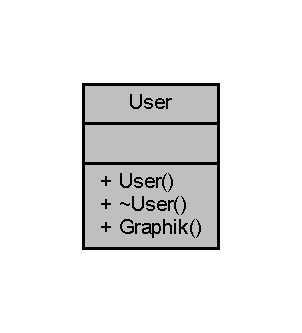
\includegraphics[width=145pt]{class_user__coll__graph}
\end{center}
\end{figure}
\subsection*{Öffentliche Methoden}
\begin{DoxyCompactItemize}
\item 
\hyperlink{class_user_a4a0137053e591fbb79d9057dd7d2283d}{User} ()
\item 
virtual \hyperlink{class_user_ac00b72ad64eb4149f7b21b9f5468c2b2}{$\sim$\+User} ()
\item 
void \hyperlink{class_user_aaf9d3a0c3d38a5f955e7b862e3ceb01c}{Graphik} ()
\end{DoxyCompactItemize}


\subsection{Ausführliche Beschreibung}
class \hyperlink{class_user}{User} 

\subsection{Beschreibung der Konstruktoren und Destruktoren}
\hypertarget{class_user_a4a0137053e591fbb79d9057dd7d2283d}{}\index{User@{User}!User@{User}}
\index{User@{User}!User@{User}}
\subsubsection[{User}]{\setlength{\rightskip}{0pt plus 5cm}User\+::\+User (
\begin{DoxyParamCaption}
{}
\end{DoxyParamCaption}
)}\label{class_user_a4a0137053e591fbb79d9057dd7d2283d}
Empty Constructor \hypertarget{class_user_ac00b72ad64eb4149f7b21b9f5468c2b2}{}\index{User@{User}!````~User@{$\sim$\+User}}
\index{````~User@{$\sim$\+User}!User@{User}}
\subsubsection[{$\sim$\+User}]{\setlength{\rightskip}{0pt plus 5cm}User\+::$\sim$\+User (
\begin{DoxyParamCaption}
{}
\end{DoxyParamCaption}
)\hspace{0.3cm}{\ttfamily [virtual]}}\label{class_user_ac00b72ad64eb4149f7b21b9f5468c2b2}
Empty Destructor 

\subsection{Dokumentation der Elementfunktionen}
\hypertarget{class_user_aaf9d3a0c3d38a5f955e7b862e3ceb01c}{}\index{User@{User}!Graphik@{Graphik}}
\index{Graphik@{Graphik}!User@{User}}
\subsubsection[{Graphik}]{\setlength{\rightskip}{0pt plus 5cm}void User\+::\+Graphik (
\begin{DoxyParamCaption}
{}
\end{DoxyParamCaption}
)}\label{class_user_aaf9d3a0c3d38a5f955e7b862e3ceb01c}


Die Dokumentation für diese Klasse wurde erzeugt aufgrund der Dateien\+:\begin{DoxyCompactItemize}
\item 
\hyperlink{_user_8h}{User.\+h}\item 
\hyperlink{_user_8cpp}{User.\+cpp}\end{DoxyCompactItemize}

\hypertarget{structzug}{}\section{zug Strukturreferenz}
\label{structzug}\index{zug@{zug}}


{\ttfamily \#include $<$zug.\+h$>$}



Zusammengehörigkeiten von zug\+:\nopagebreak
\begin{figure}[H]
\begin{center}
\leavevmode
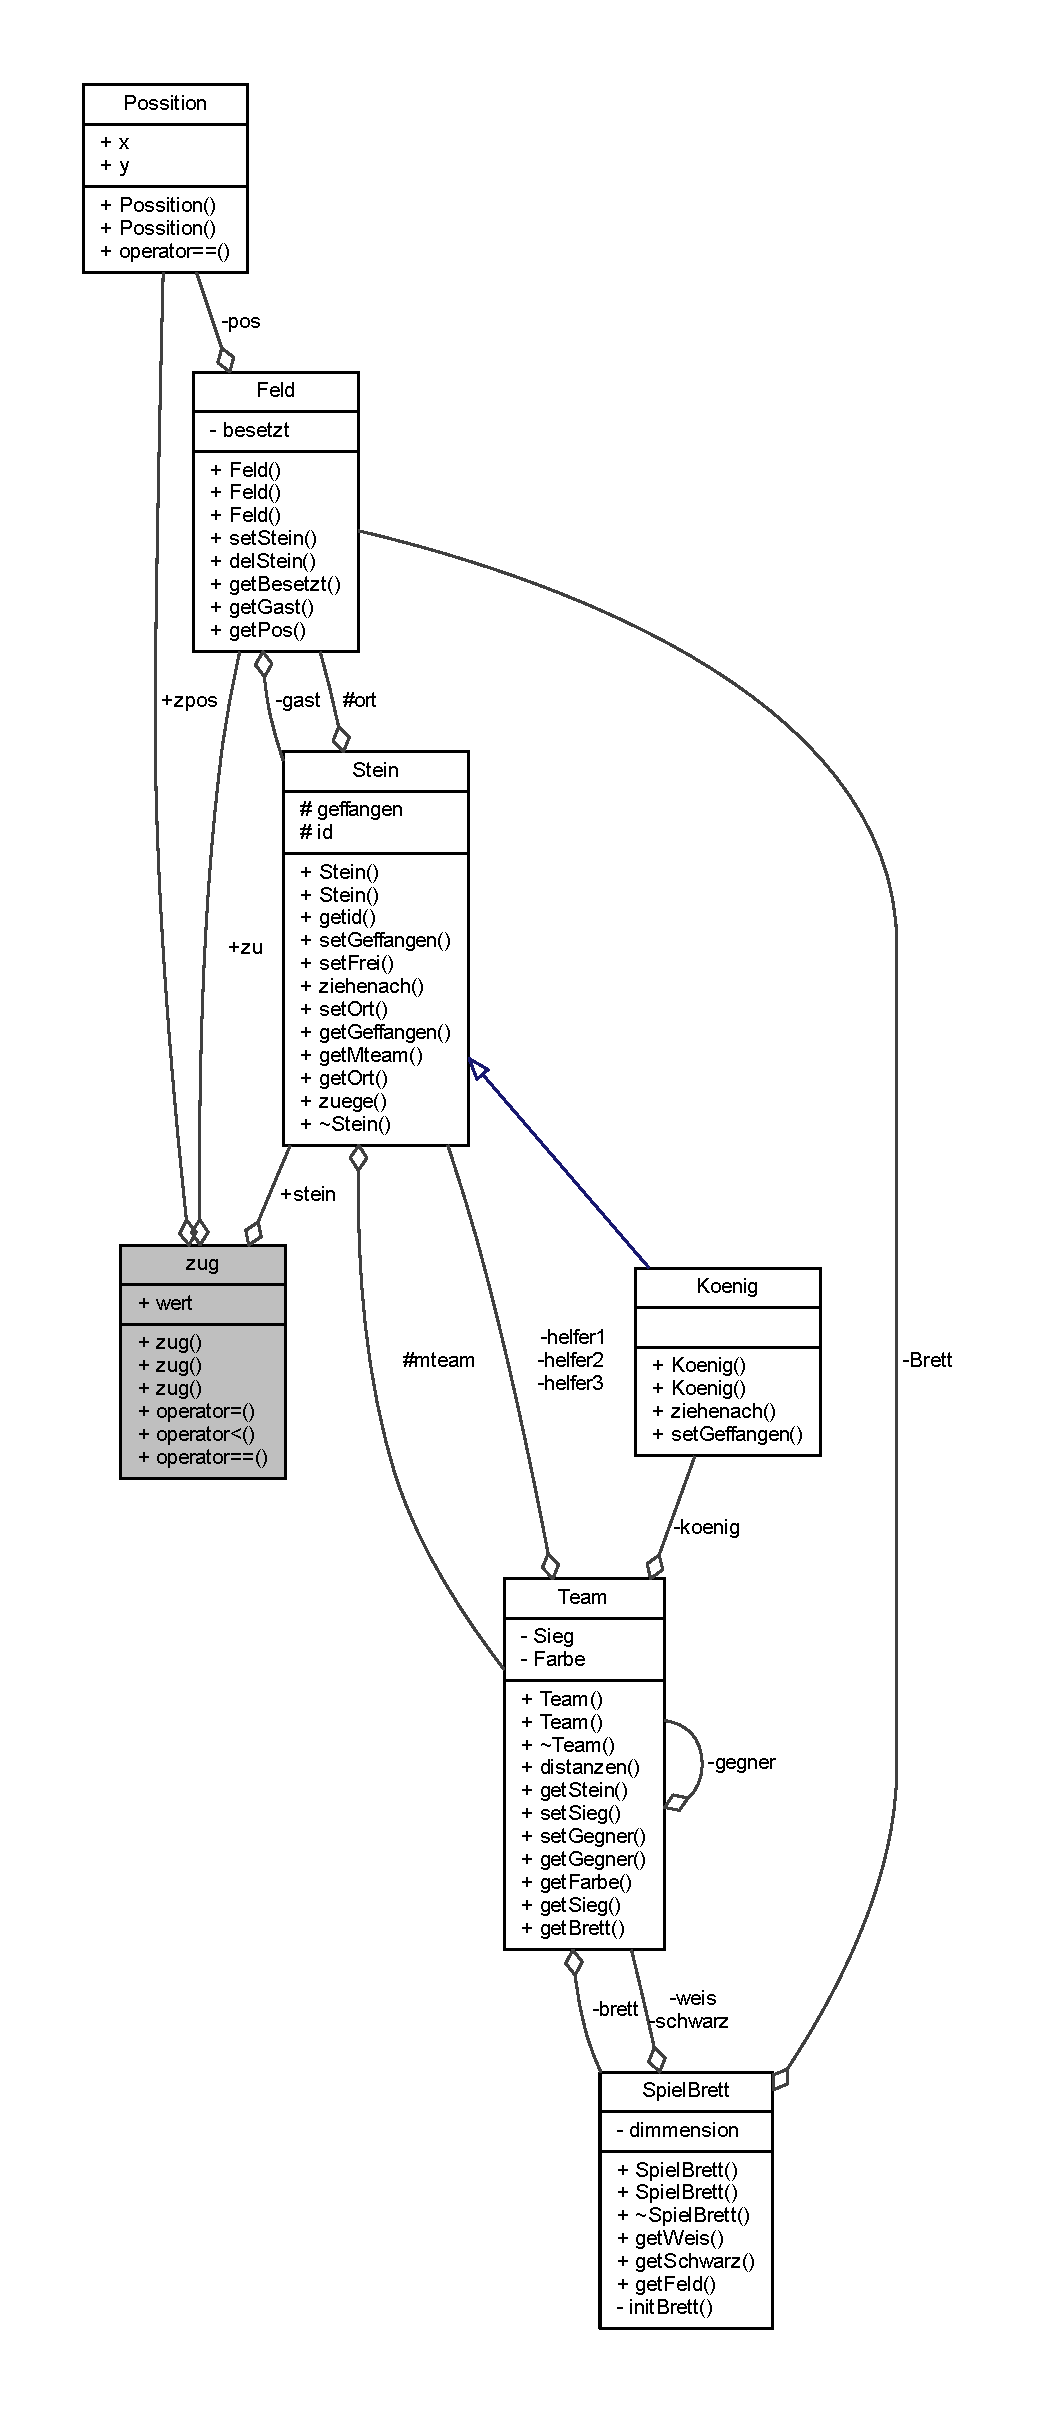
\includegraphics[height=550pt]{structzug__coll__graph}
\end{center}
\end{figure}
\subsection*{Öffentliche Methoden}
\begin{DoxyCompactItemize}
\item 
\hyperlink{structzug_ad28714c8da822cfa7324650d90e30947}{zug} ()=default
\item 
\hyperlink{structzug_ab089a9829071c1c2a242cef95b399e39}{zug} (\hyperlink{class_feld}{Feld} $\ast$z, \hyperlink{class_stein}{Stein} $\ast$s)
\item 
\hyperlink{structzug_aa390b6ca5a719bb107a66bd6ddb728f6}{zug} (const \hyperlink{structzug}{zug} \&z)
\item 
\hyperlink{structzug}{zug} \& \hyperlink{structzug_aee196f37d4c013c82c89715a09e63d75}{operator=} (const \hyperlink{structzug}{zug} \&z)
\item 
bool \hyperlink{structzug_afd3240046f4e7e9fb7495b1eee259d35}{operator$<$} (const \hyperlink{structzug}{zug} \&z) const 
\item 
bool \hyperlink{structzug_a5676590b96c8d14da3ca588718af33d7}{operator==} (const \hyperlink{structzug}{zug} \&z) const 
\end{DoxyCompactItemize}
\subsection*{Öffentliche Attribute}
\begin{DoxyCompactItemize}
\item 
\hyperlink{class_feld}{Feld} $\ast$ \hyperlink{structzug_aa1d47432b331308a510572187bfbe0ec}{zu} =nullptr
\item 
\hyperlink{class_stein}{Stein} $\ast$ \hyperlink{structzug_a4b431b73a9dbcfd9b2c20afb66f76998}{stein} =nullptr
\item 
int \hyperlink{structzug_adea5273c99ffd5fb46a9f5367a0fef3e}{wert} =100
\item 
\hyperlink{struct_possition}{Possition} \hyperlink{structzug_a849eec23abc7f17b4241197f48683bc8}{zpos}
\end{DoxyCompactItemize}


\subsection{Ausführliche Beschreibung}
struct Zug Daten Struktur die einen Spiel-\/\+Zug Symbolysiert. 

\subsection{Beschreibung der Konstruktoren und Destruktoren}
\hypertarget{structzug_ad28714c8da822cfa7324650d90e30947}{}\index{zug@{zug}!zug@{zug}}
\index{zug@{zug}!zug@{zug}}
\subsubsection[{zug}]{\setlength{\rightskip}{0pt plus 5cm}zug\+::zug (
\begin{DoxyParamCaption}
{}
\end{DoxyParamCaption}
)\hspace{0.3cm}{\ttfamily [default]}}\label{structzug_ad28714c8da822cfa7324650d90e30947}
\hypertarget{structzug_ab089a9829071c1c2a242cef95b399e39}{}\index{zug@{zug}!zug@{zug}}
\index{zug@{zug}!zug@{zug}}
\subsubsection[{zug}]{\setlength{\rightskip}{0pt plus 5cm}zug\+::zug (
\begin{DoxyParamCaption}
\item[{{\bf Feld} $\ast$}]{z, }
\item[{{\bf Stein} $\ast$}]{s}
\end{DoxyParamCaption}
)\hspace{0.3cm}{\ttfamily [inline]}}\label{structzug_ab089a9829071c1c2a242cef95b399e39}
\hypertarget{structzug_aa390b6ca5a719bb107a66bd6ddb728f6}{}\index{zug@{zug}!zug@{zug}}
\index{zug@{zug}!zug@{zug}}
\subsubsection[{zug}]{\setlength{\rightskip}{0pt plus 5cm}zug\+::zug (
\begin{DoxyParamCaption}
\item[{const {\bf zug} \&}]{z}
\end{DoxyParamCaption}
)\hspace{0.3cm}{\ttfamily [inline]}}\label{structzug_aa390b6ca5a719bb107a66bd6ddb728f6}


\subsection{Dokumentation der Elementfunktionen}
\hypertarget{structzug_afd3240046f4e7e9fb7495b1eee259d35}{}\index{zug@{zug}!operator$<$@{operator$<$}}
\index{operator$<$@{operator$<$}!zug@{zug}}
\subsubsection[{operator$<$}]{\setlength{\rightskip}{0pt plus 5cm}bool zug\+::operator$<$ (
\begin{DoxyParamCaption}
\item[{const {\bf zug} \&}]{z}
\end{DoxyParamCaption}
) const\hspace{0.3cm}{\ttfamily [inline]}}\label{structzug_afd3240046f4e7e9fb7495b1eee259d35}
Kleiner als Operator Vergleicht Zuege nach Wertigkeit; 
\begin{DoxyParams}{Parameter}
{\em z} & \\
\hline
\end{DoxyParams}
\begin{DoxyReturn}{Rückgabe}

\end{DoxyReturn}
\hypertarget{structzug_aee196f37d4c013c82c89715a09e63d75}{}\index{zug@{zug}!operator=@{operator=}}
\index{operator=@{operator=}!zug@{zug}}
\subsubsection[{operator=}]{\setlength{\rightskip}{0pt plus 5cm}{\bf zug}\& zug\+::operator= (
\begin{DoxyParamCaption}
\item[{const {\bf zug} \&}]{z}
\end{DoxyParamCaption}
)\hspace{0.3cm}{\ttfamily [inline]}}\label{structzug_aee196f37d4c013c82c89715a09e63d75}
\hypertarget{structzug_a5676590b96c8d14da3ca588718af33d7}{}\index{zug@{zug}!operator==@{operator==}}
\index{operator==@{operator==}!zug@{zug}}
\subsubsection[{operator==}]{\setlength{\rightskip}{0pt plus 5cm}bool zug\+::operator== (
\begin{DoxyParamCaption}
\item[{const {\bf zug} \&}]{z}
\end{DoxyParamCaption}
) const\hspace{0.3cm}{\ttfamily [inline]}}\label{structzug_a5676590b96c8d14da3ca588718af33d7}
Vergleichs-\/\+Operator Vergleicht Zuege auf gleiche Ziel-\/\+Position 
\begin{DoxyParams}{Parameter}
{\em z} & \\
\hline
\end{DoxyParams}
\begin{DoxyReturn}{Rückgabe}

\end{DoxyReturn}


\subsection{Dokumentation der Datenelemente}
\hypertarget{structzug_a4b431b73a9dbcfd9b2c20afb66f76998}{}\index{zug@{zug}!stein@{stein}}
\index{stein@{stein}!zug@{zug}}
\subsubsection[{stein}]{\setlength{\rightskip}{0pt plus 5cm}{\bf Stein}$\ast$ zug\+::stein =nullptr}\label{structzug_a4b431b73a9dbcfd9b2c20afb66f76998}
\hypertarget{structzug_adea5273c99ffd5fb46a9f5367a0fef3e}{}\index{zug@{zug}!wert@{wert}}
\index{wert@{wert}!zug@{zug}}
\subsubsection[{wert}]{\setlength{\rightskip}{0pt plus 5cm}int zug\+::wert =100}\label{structzug_adea5273c99ffd5fb46a9f5367a0fef3e}
\hypertarget{structzug_a849eec23abc7f17b4241197f48683bc8}{}\index{zug@{zug}!zpos@{zpos}}
\index{zpos@{zpos}!zug@{zug}}
\subsubsection[{zpos}]{\setlength{\rightskip}{0pt plus 5cm}{\bf Possition} zug\+::zpos}\label{structzug_a849eec23abc7f17b4241197f48683bc8}
\hypertarget{structzug_aa1d47432b331308a510572187bfbe0ec}{}\index{zug@{zug}!zu@{zu}}
\index{zu@{zu}!zug@{zug}}
\subsubsection[{zu}]{\setlength{\rightskip}{0pt plus 5cm}{\bf Feld}$\ast$ zug\+::zu =nullptr}\label{structzug_aa1d47432b331308a510572187bfbe0ec}


Die Dokumentation für diese Struktur wurde erzeugt aufgrund der Datei\+:\begin{DoxyCompactItemize}
\item 
\hyperlink{zug_8h}{zug.\+h}\end{DoxyCompactItemize}

\chapter{Datei-\/\+Dokumentation}
\hypertarget{_feld_8cpp}{}\section{Feld.\+cpp-\/\+Dateireferenz}
\label{_feld_8cpp}\index{Feld.\+cpp@{Feld.\+cpp}}
{\ttfamily \#include \char`\"{}../h/\+Feld.\+h\char`\"{}}\\*
Include-\/\+Abhängigkeitsdiagramm für Feld.\+cpp\+:\nopagebreak
\begin{figure}[H]
\begin{center}
\leavevmode
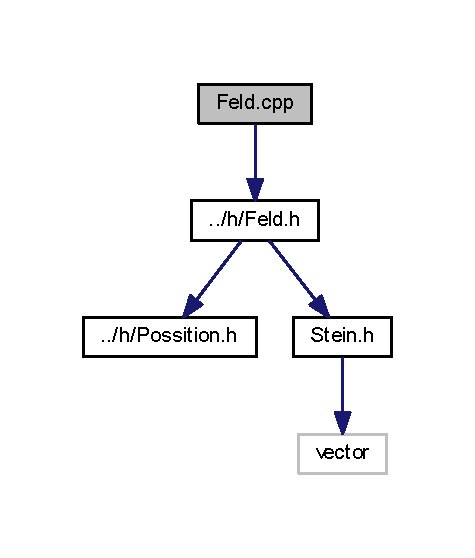
\includegraphics[width=228pt]{_feld_8cpp__incl}
\end{center}
\end{figure}
\subsection*{Makrodefinitionen}
\begin{DoxyCompactItemize}
\item 
\#define \hyperlink{_feld_8cpp_ae135a65f6420a0cb5f9f48311cec5bff}{S\+T\+E\+I\+N\+\_\+\+C}
\end{DoxyCompactItemize}


\subsection{Makro-\/\+Dokumentation}
\hypertarget{_feld_8cpp_ae135a65f6420a0cb5f9f48311cec5bff}{}\index{Feld.\+cpp@{Feld.\+cpp}!S\+T\+E\+I\+N\+\_\+\+C@{S\+T\+E\+I\+N\+\_\+\+C}}
\index{S\+T\+E\+I\+N\+\_\+\+C@{S\+T\+E\+I\+N\+\_\+\+C}!Feld.\+cpp@{Feld.\+cpp}}
\subsubsection[{S\+T\+E\+I\+N\+\_\+\+C}]{\setlength{\rightskip}{0pt plus 5cm}\#define S\+T\+E\+I\+N\+\_\+\+C}\label{_feld_8cpp_ae135a65f6420a0cb5f9f48311cec5bff}

\hypertarget{_feld_8h}{}\section{Feld.\+h-\/\+Dateireferenz}
\label{_feld_8h}\index{Feld.\+h@{Feld.\+h}}
{\ttfamily \#include \char`\"{}../h/\+Possition.\+h\char`\"{}}\\*
{\ttfamily \#include \char`\"{}Stein.\+h\char`\"{}}\\*
Include-\/\+Abhängigkeitsdiagramm für Feld.\+h\+:\nopagebreak
\begin{figure}[H]
\begin{center}
\leavevmode
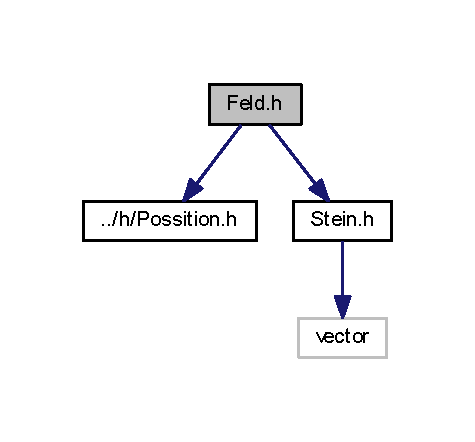
\includegraphics[width=228pt]{_feld_8h__incl}
\end{center}
\end{figure}
Dieser Graph zeigt, welche Datei direkt oder indirekt diese Datei enthält\+:\nopagebreak
\begin{figure}[H]
\begin{center}
\leavevmode
\includegraphics[width=350pt]{_feld_8h__dep__incl}
\end{center}
\end{figure}
\subsection*{Klassen}
\begin{DoxyCompactItemize}
\item 
class \hyperlink{class_feld}{Feld}
\end{DoxyCompactItemize}

\hypertarget{_g_u_i_8cpp}{}\section{G\+U\+I.\+cpp-\/\+Dateireferenz}
\label{_g_u_i_8cpp}\index{G\+U\+I.\+cpp@{G\+U\+I.\+cpp}}
{\ttfamily \#include \char`\"{}../h/\+G\+U\+I.\+h\char`\"{}}\\*
{\ttfamily \#include $<$iostream$>$}\\*
{\ttfamily \#include $<$windows.\+h$>$}\\*
{\ttfamily \#include $<$stdlib.\+h$>$}\\*
{\ttfamily \#include \char`\"{}../h/\+K\+I.\+h\char`\"{}}\\*
{\ttfamily \#include \char`\"{}../h/\+Spielbrett.\+h\char`\"{}}\\*
{\ttfamily \#include \char`\"{}../h/\+Stein.\+h\char`\"{}}\\*
Include-\/\+Abhängigkeitsdiagramm für G\+U\+I.\+cpp\+:\nopagebreak
\begin{figure}[H]
\begin{center}
\leavevmode
\includegraphics[width=350pt]{_g_u_i_8cpp__incl}
\end{center}
\end{figure}

\hypertarget{_g_u_i_8h}{}\section{G\+U\+I.\+h-\/\+Dateireferenz}
\label{_g_u_i_8h}\index{G\+U\+I.\+h@{G\+U\+I.\+h}}
{\ttfamily \#include \char`\"{}Spiel\+Brett.\+h\char`\"{}}\\*
{\ttfamily \#include \char`\"{}../h/\+K\+I.\+h\char`\"{}}\\*
Include-\/\+Abhängigkeitsdiagramm für G\+U\+I.\+h\+:\nopagebreak
\begin{figure}[H]
\begin{center}
\leavevmode
\includegraphics[width=350pt]{_g_u_i_8h__incl}
\end{center}
\end{figure}
Dieser Graph zeigt, welche Datei direkt oder indirekt diese Datei enthält\+:\nopagebreak
\begin{figure}[H]
\begin{center}
\leavevmode
\includegraphics[width=206pt]{_g_u_i_8h__dep__incl}
\end{center}
\end{figure}
\subsection*{Klassen}
\begin{DoxyCompactItemize}
\item 
class \hyperlink{class_g_u_i}{G\+U\+I}
\end{DoxyCompactItemize}

\hypertarget{_k_i_8cpp}{}\section{K\+I.\+cpp-\/\+Dateireferenz}
\label{_k_i_8cpp}\index{K\+I.\+cpp@{K\+I.\+cpp}}
{\ttfamily \#include \char`\"{}../h/\+K\+I.\+h\char`\"{}}\\*
{\ttfamily \#include \char`\"{}../h/\+Sf\+K.\+h\char`\"{}}\\*
{\ttfamily \#include \char`\"{}../h/\+Ss\+K.\+h\char`\"{}}\\*
{\ttfamily \#include \char`\"{}../h/\+Sf\+H.\+h\char`\"{}}\\*
{\ttfamily \#include \char`\"{}../h/\+Sr\+H.\+h\char`\"{}}\\*
{\ttfamily \#include \char`\"{}../h/\+Strategie.\+h\char`\"{}}\\*
{\ttfamily \#include $<$iostream$>$}\\*
{\ttfamily \#include $<$cstdlib$>$}\\*
{\ttfamily \#include $<$time.\+h$>$}\\*
{\ttfamily \#include $<$algorithm$>$}\\*
Include-\/\+Abhängigkeitsdiagramm für K\+I.\+cpp\+:\nopagebreak
\begin{figure}[H]
\begin{center}
\leavevmode
\includegraphics[width=350pt]{_k_i_8cpp__incl}
\end{center}
\end{figure}

\hypertarget{_k_i_8h}{}\section{K\+I.\+h-\/\+Dateireferenz}
\label{_k_i_8h}\index{K\+I.\+h@{K\+I.\+h}}
{\ttfamily \#include \char`\"{}Team.\+h\char`\"{}}\\*
{\ttfamily \#include \char`\"{}Spiel\+Brett.\+h\char`\"{}}\\*
{\ttfamily \#include \char`\"{}zug.\+h\char`\"{}}\\*
{\ttfamily \#include \char`\"{}Ss\+K.\+h\char`\"{}}\\*
Include-\/\+Abhängigkeitsdiagramm für K\+I.\+h\+:\nopagebreak
\begin{figure}[H]
\begin{center}
\leavevmode
\includegraphics[width=350pt]{_k_i_8h__incl}
\end{center}
\end{figure}
Dieser Graph zeigt, welche Datei direkt oder indirekt diese Datei enthält\+:\nopagebreak
\begin{figure}[H]
\begin{center}
\leavevmode
\includegraphics[width=270pt]{_k_i_8h__dep__incl}
\end{center}
\end{figure}
\subsection*{Klassen}
\begin{DoxyCompactItemize}
\item 
class \hyperlink{class_k_i}{K\+I}
\end{DoxyCompactItemize}

\hypertarget{_koenig_8cpp}{}\section{Koenig.\+cpp-\/\+Dateireferenz}
\label{_koenig_8cpp}\index{Koenig.\+cpp@{Koenig.\+cpp}}
{\ttfamily \#include \char`\"{}../h/\+Koenig.\+h\char`\"{}}\\*
{\ttfamily \#include \char`\"{}../h/\+Feld.\+h\char`\"{}}\\*
{\ttfamily \#include \char`\"{}../h/\+Team.\+h\char`\"{}}\\*
Include-\/\+Abhängigkeitsdiagramm für Koenig.\+cpp\+:\nopagebreak
\begin{figure}[H]
\begin{center}
\leavevmode
\includegraphics[width=325pt]{_koenig_8cpp__incl}
\end{center}
\end{figure}
\subsection*{Makrodefinitionen}
\begin{DoxyCompactItemize}
\item 
\#define \hyperlink{_koenig_8cpp_ad27cd45567deccd6153eb0e1ed2c8df9}{K\+O\+E\+I\+N\+G\+\_\+\+C}
\end{DoxyCompactItemize}


\subsection{Makro-\/\+Dokumentation}
\hypertarget{_koenig_8cpp_ad27cd45567deccd6153eb0e1ed2c8df9}{}\index{Koenig.\+cpp@{Koenig.\+cpp}!K\+O\+E\+I\+N\+G\+\_\+\+C@{K\+O\+E\+I\+N\+G\+\_\+\+C}}
\index{K\+O\+E\+I\+N\+G\+\_\+\+C@{K\+O\+E\+I\+N\+G\+\_\+\+C}!Koenig.\+cpp@{Koenig.\+cpp}}
\subsubsection[{K\+O\+E\+I\+N\+G\+\_\+\+C}]{\setlength{\rightskip}{0pt plus 5cm}\#define K\+O\+E\+I\+N\+G\+\_\+\+C}\label{_koenig_8cpp_ad27cd45567deccd6153eb0e1ed2c8df9}

\hypertarget{_koenig_8h}{}\section{Koenig.\+h-\/\+Dateireferenz}
\label{_koenig_8h}\index{Koenig.\+h@{Koenig.\+h}}
{\ttfamily \#include \char`\"{}Stein.\+h\char`\"{}}\\*
Include-\/\+Abhängigkeitsdiagramm für Koenig.\+h\+:\nopagebreak
\begin{figure}[H]
\begin{center}
\leavevmode
\includegraphics[width=135pt]{_koenig_8h__incl}
\end{center}
\end{figure}
Dieser Graph zeigt, welche Datei direkt oder indirekt diese Datei enthält\+:\nopagebreak
\begin{figure}[H]
\begin{center}
\leavevmode
\includegraphics[width=222pt]{_koenig_8h__dep__incl}
\end{center}
\end{figure}
\subsection*{Klassen}
\begin{DoxyCompactItemize}
\item 
class \hyperlink{class_koenig}{Koenig}
\end{DoxyCompactItemize}
\subsection*{Makrodefinitionen}
\begin{DoxyCompactItemize}
\item 
\#define \hyperlink{_koenig_8h_aad08d2740e17e6c23dfee187c1ffef70}{K\+O\+E\+N\+I\+G\+\_\+\+H}
\end{DoxyCompactItemize}


\subsection{Makro-\/\+Dokumentation}
\hypertarget{_koenig_8h_aad08d2740e17e6c23dfee187c1ffef70}{}\index{Koenig.\+h@{Koenig.\+h}!K\+O\+E\+N\+I\+G\+\_\+\+H@{K\+O\+E\+N\+I\+G\+\_\+\+H}}
\index{K\+O\+E\+N\+I\+G\+\_\+\+H@{K\+O\+E\+N\+I\+G\+\_\+\+H}!Koenig.\+h@{Koenig.\+h}}
\subsubsection[{K\+O\+E\+N\+I\+G\+\_\+\+H}]{\setlength{\rightskip}{0pt plus 5cm}\#define K\+O\+E\+N\+I\+G\+\_\+\+H}\label{_koenig_8h_aad08d2740e17e6c23dfee187c1ffef70}

\hypertarget{main_8cpp}{}\section{main.\+cpp-\/\+Dateireferenz}
\label{main_8cpp}\index{main.\+cpp@{main.\+cpp}}
{\ttfamily \#include $<$windows.\+h$>$}\\*
{\ttfamily \#include $<$iostream$>$}\\*
{\ttfamily \#include $<$memory$>$}\\*
{\ttfamily \#include \char`\"{}../h/\+Spielbrett.\+h\char`\"{}}\\*
{\ttfamily \#include $<$stdlib.\+h$>$}\\*
{\ttfamily \#include \char`\"{}../h/\+K\+I.\+h\char`\"{}}\\*
{\ttfamily \#include \char`\"{}../h/\+G\+U\+I.\+h\char`\"{}}\\*
{\ttfamily \#include \char`\"{}../h/\+Stein.\+h\char`\"{}}\\*
Include-\/\+Abhängigkeitsdiagramm für main.\+cpp\+:\nopagebreak
\begin{figure}[H]
\begin{center}
\leavevmode
\includegraphics[width=350pt]{main_8cpp__incl}
\end{center}
\end{figure}
\subsection*{Funktionen}
\begin{DoxyCompactItemize}
\item 
int \hyperlink{main_8cpp_a2b86bba34879dd3c93ed0ea4abce467a}{main} (int \+\_\+argc, char $\ast$argv\mbox{[}$\,$\mbox{]})
\end{DoxyCompactItemize}


\subsection{Dokumentation der Funktionen}
\hypertarget{main_8cpp_a2b86bba34879dd3c93ed0ea4abce467a}{}\index{main.\+cpp@{main.\+cpp}!main@{main}}
\index{main@{main}!main.\+cpp@{main.\+cpp}}
\subsubsection[{main}]{\setlength{\rightskip}{0pt plus 5cm}int main (
\begin{DoxyParamCaption}
\item[{int}]{\+\_\+argc, }
\item[{char $\ast$}]{argv\mbox{[}$\,$\mbox{]}}
\end{DoxyParamCaption}
)}\label{main_8cpp_a2b86bba34879dd3c93ed0ea4abce467a}


Hier ist ein Graph, der zeigt, was diese Funktion aufruft\+:\nopagebreak
\begin{figure}[H]
\begin{center}
\leavevmode
\includegraphics[width=267pt]{main_8cpp_a2b86bba34879dd3c93ed0ea4abce467a_cgraph}
\end{center}
\end{figure}



\hypertarget{_main_8h}{}\section{Main.\+h-\/\+Dateireferenz}
\label{_main_8h}\index{Main.\+h@{Main.\+h}}

\hypertarget{_possition_8h}{}\section{Possition.\+h-\/\+Dateireferenz}
\label{_possition_8h}\index{Possition.\+h@{Possition.\+h}}
Dieser Graph zeigt, welche Datei direkt oder indirekt diese Datei enthält\+:\nopagebreak
\begin{figure}[H]
\begin{center}
\leavevmode
\includegraphics[width=350pt]{_possition_8h__dep__incl}
\end{center}
\end{figure}
\subsection*{Klassen}
\begin{DoxyCompactItemize}
\item 
struct \hyperlink{struct_possition}{Possition}
\end{DoxyCompactItemize}
\subsection*{Makrodefinitionen}
\begin{DoxyCompactItemize}
\item 
\#define \hyperlink{_possition_8h_ac9fb942d51fb8f89dd86b3eca68d6135}{P\+O\+S\+S\+I\+T\+I\+O\+N\+\_\+\+H}
\end{DoxyCompactItemize}


\subsection{Makro-\/\+Dokumentation}
\hypertarget{_possition_8h_ac9fb942d51fb8f89dd86b3eca68d6135}{}\index{Possition.\+h@{Possition.\+h}!P\+O\+S\+S\+I\+T\+I\+O\+N\+\_\+\+H@{P\+O\+S\+S\+I\+T\+I\+O\+N\+\_\+\+H}}
\index{P\+O\+S\+S\+I\+T\+I\+O\+N\+\_\+\+H@{P\+O\+S\+S\+I\+T\+I\+O\+N\+\_\+\+H}!Possition.\+h@{Possition.\+h}}
\subsubsection[{P\+O\+S\+S\+I\+T\+I\+O\+N\+\_\+\+H}]{\setlength{\rightskip}{0pt plus 5cm}\#define P\+O\+S\+S\+I\+T\+I\+O\+N\+\_\+\+H}\label{_possition_8h_ac9fb942d51fb8f89dd86b3eca68d6135}

\hypertarget{_sf_h_8cpp}{}\section{Sf\+H.\+cpp-\/\+Dateireferenz}
\label{_sf_h_8cpp}\index{Sf\+H.\+cpp@{Sf\+H.\+cpp}}
{\ttfamily \#include \char`\"{}../h/\+Sf\+H.\+h\char`\"{}}\\*
{\ttfamily \#include $<$algorithm$>$}\\*
Include-\/\+Abhängigkeitsdiagramm für Sf\+H.\+cpp\+:\nopagebreak
\begin{figure}[H]
\begin{center}
\leavevmode
\includegraphics[width=327pt]{_sf_h_8cpp__incl}
\end{center}
\end{figure}

\hypertarget{_sf_h_8h}{}\section{Sf\+H.\+h-\/\+Dateireferenz}
\label{_sf_h_8h}\index{Sf\+H.\+h@{Sf\+H.\+h}}
{\ttfamily \#include \char`\"{}Strategie.\+h\char`\"{}}\\*
Include-\/\+Abhängigkeitsdiagramm für Sf\+H.\+h\+:\nopagebreak
\begin{figure}[H]
\begin{center}
\leavevmode
\includegraphics[width=327pt]{_sf_h_8h__incl}
\end{center}
\end{figure}
Dieser Graph zeigt, welche Datei direkt oder indirekt diese Datei enthält\+:\nopagebreak
\begin{figure}[H]
\begin{center}
\leavevmode
\includegraphics[width=194pt]{_sf_h_8h__dep__incl}
\end{center}
\end{figure}
\subsection*{Klassen}
\begin{DoxyCompactItemize}
\item 
class \hyperlink{class_sf_h}{Sf\+H}
\end{DoxyCompactItemize}

\hypertarget{_sf_k_8cpp}{}\section{Sf\+K.\+cpp-\/\+Dateireferenz}
\label{_sf_k_8cpp}\index{Sf\+K.\+cpp@{Sf\+K.\+cpp}}
{\ttfamily \#include \char`\"{}../h/\+Sf\+K.\+h\char`\"{}}\\*
{\ttfamily \#include $<$cmath$>$}\\*
{\ttfamily \#include $<$algorithm$>$}\\*
{\ttfamily \#include \char`\"{}../h/zug.\+h\char`\"{}}\\*
{\ttfamily \#include $<$iostream$>$}\\*
Include-\/\+Abhängigkeitsdiagramm für Sf\+K.\+cpp\+:\nopagebreak
\begin{figure}[H]
\begin{center}
\leavevmode
\includegraphics[width=350pt]{_sf_k_8cpp__incl}
\end{center}
\end{figure}

\hypertarget{_sf_k_8h}{}\section{Sf\+K.\+h-\/\+Dateireferenz}
\label{_sf_k_8h}\index{Sf\+K.\+h@{Sf\+K.\+h}}
{\ttfamily \#include \char`\"{}Team.\+h\char`\"{}}\\*
{\ttfamily \#include \char`\"{}Spiel\+Brett.\+h\char`\"{}}\\*
{\ttfamily \#include \char`\"{}Strategie.\+h\char`\"{}}\\*
Include-\/\+Abhängigkeitsdiagramm für Sf\+K.\+h\+:\nopagebreak
\begin{figure}[H]
\begin{center}
\leavevmode
\includegraphics[width=350pt]{_sf_k_8h__incl}
\end{center}
\end{figure}
Dieser Graph zeigt, welche Datei direkt oder indirekt diese Datei enthält\+:\nopagebreak
\begin{figure}[H]
\begin{center}
\leavevmode
\includegraphics[width=350pt]{_sf_k_8h__dep__incl}
\end{center}
\end{figure}
\subsection*{Klassen}
\begin{DoxyCompactItemize}
\item 
class \hyperlink{class_sf_k}{Sf\+K}
\end{DoxyCompactItemize}

\hypertarget{_spiel_brett_8cpp}{}\section{Spiel\+Brett.\+cpp-\/\+Dateireferenz}
\label{_spiel_brett_8cpp}\index{Spiel\+Brett.\+cpp@{Spiel\+Brett.\+cpp}}
{\ttfamily \#include $<$stdlib.\+h$>$}\\*
{\ttfamily \#include $<$iostream$>$}\\*
{\ttfamily \#include \char`\"{}../h/\+Spiel\+Brett.\+h\char`\"{}}\\*
Include-\/\+Abhängigkeitsdiagramm für Spiel\+Brett.\+cpp\+:\nopagebreak
\begin{figure}[H]
\begin{center}
\leavevmode
\includegraphics[width=304pt]{_spiel_brett_8cpp__incl}
\end{center}
\end{figure}
\subsection*{Makrodefinitionen}
\begin{DoxyCompactItemize}
\item 
\#define \hyperlink{_spiel_brett_8cpp_a6169dde86b5facdf91186f6c93394b9a}{S\+P\+I\+E\+L\+B\+R\+E\+T\+T\+\_\+\+C}
\end{DoxyCompactItemize}


\subsection{Makro-\/\+Dokumentation}
\hypertarget{_spiel_brett_8cpp_a6169dde86b5facdf91186f6c93394b9a}{}\index{Spiel\+Brett.\+cpp@{Spiel\+Brett.\+cpp}!S\+P\+I\+E\+L\+B\+R\+E\+T\+T\+\_\+\+C@{S\+P\+I\+E\+L\+B\+R\+E\+T\+T\+\_\+\+C}}
\index{S\+P\+I\+E\+L\+B\+R\+E\+T\+T\+\_\+\+C@{S\+P\+I\+E\+L\+B\+R\+E\+T\+T\+\_\+\+C}!Spiel\+Brett.\+cpp@{Spiel\+Brett.\+cpp}}
\subsubsection[{S\+P\+I\+E\+L\+B\+R\+E\+T\+T\+\_\+\+C}]{\setlength{\rightskip}{0pt plus 5cm}\#define S\+P\+I\+E\+L\+B\+R\+E\+T\+T\+\_\+\+C}\label{_spiel_brett_8cpp_a6169dde86b5facdf91186f6c93394b9a}

\hypertarget{_spiel_brett_8h}{}\section{Spiel\+Brett.\+h-\/\+Dateireferenz}
\label{_spiel_brett_8h}\index{Spiel\+Brett.\+h@{Spiel\+Brett.\+h}}
{\ttfamily \#include \char`\"{}Feld.\+h\char`\"{}}\\*
{\ttfamily \#include \char`\"{}Team.\+h\char`\"{}}\\*
Include-\/\+Abhängigkeitsdiagramm für Spiel\+Brett.\+h\+:\nopagebreak
\begin{figure}[H]
\begin{center}
\leavevmode
\includegraphics[width=291pt]{_spiel_brett_8h__incl}
\end{center}
\end{figure}
Dieser Graph zeigt, welche Datei direkt oder indirekt diese Datei enthält\+:\nopagebreak
\begin{figure}[H]
\begin{center}
\leavevmode
\includegraphics[width=350pt]{_spiel_brett_8h__dep__incl}
\end{center}
\end{figure}
\subsection*{Klassen}
\begin{DoxyCompactItemize}
\item 
class \hyperlink{class_spiel_brett}{Spiel\+Brett}
\end{DoxyCompactItemize}

\hypertarget{_sr_h_8cpp}{}\section{Sr\+H.\+cpp-\/\+Dateireferenz}
\label{_sr_h_8cpp}\index{Sr\+H.\+cpp@{Sr\+H.\+cpp}}
{\ttfamily \#include \char`\"{}../h/\+Sr\+H.\+h\char`\"{}}\\*
{\ttfamily \#include $<$algorithm$>$}\\*
Include-\/\+Abhängigkeitsdiagramm für Sr\+H.\+cpp\+:\nopagebreak
\begin{figure}[H]
\begin{center}
\leavevmode
\includegraphics[width=327pt]{_sr_h_8cpp__incl}
\end{center}
\end{figure}

\hypertarget{_sr_h_8h}{}\section{Sr\+H.\+h-\/\+Dateireferenz}
\label{_sr_h_8h}\index{Sr\+H.\+h@{Sr\+H.\+h}}
{\ttfamily \#include \char`\"{}Strategie.\+h\char`\"{}}\\*
Include-\/\+Abhängigkeitsdiagramm für Sr\+H.\+h\+:\nopagebreak
\begin{figure}[H]
\begin{center}
\leavevmode
\includegraphics[width=327pt]{_sr_h_8h__incl}
\end{center}
\end{figure}
Dieser Graph zeigt, welche Datei direkt oder indirekt diese Datei enthält\+:\nopagebreak
\begin{figure}[H]
\begin{center}
\leavevmode
\includegraphics[width=194pt]{_sr_h_8h__dep__incl}
\end{center}
\end{figure}
\subsection*{Klassen}
\begin{DoxyCompactItemize}
\item 
class \hyperlink{class_sr_h}{Sr\+H}
\end{DoxyCompactItemize}

\hypertarget{_ss_k_8cpp}{}\section{Ss\+K.\+cpp-\/\+Dateireferenz}
\label{_ss_k_8cpp}\index{Ss\+K.\+cpp@{Ss\+K.\+cpp}}
{\ttfamily \#include \char`\"{}../h/\+Ss\+K.\+h\char`\"{}}\\*
{\ttfamily \#include $<$cmath$>$}\\*
{\ttfamily \#include $<$algorithm$>$}\\*
{\ttfamily \#include \char`\"{}../h/zug.\+h\char`\"{}}\\*
{\ttfamily \#include \char`\"{}../h/\+Spiel\+Brett.\+h\char`\"{}}\\*
{\ttfamily \#include \char`\"{}../h/\+Team.\+h\char`\"{}}\\*
{\ttfamily \#include $<$iostream$>$}\\*
Include-\/\+Abhängigkeitsdiagramm für Ss\+K.\+cpp\+:\nopagebreak
\begin{figure}[H]
\begin{center}
\leavevmode
\includegraphics[width=350pt]{_ss_k_8cpp__incl}
\end{center}
\end{figure}

\hypertarget{_ss_k_8h}{}\section{Ss\+K.\+h-\/\+Dateireferenz}
\label{_ss_k_8h}\index{Ss\+K.\+h@{Ss\+K.\+h}}
{\ttfamily \#include \char`\"{}Strategie.\+h\char`\"{}}\\*
{\ttfamily \#include \char`\"{}Sf\+K.\+h\char`\"{}}\\*
Include-\/\+Abhängigkeitsdiagramm für Ss\+K.\+h\+:\nopagebreak
\begin{figure}[H]
\begin{center}
\leavevmode
\includegraphics[width=350pt]{_ss_k_8h__incl}
\end{center}
\end{figure}
Dieser Graph zeigt, welche Datei direkt oder indirekt diese Datei enthält\+:\nopagebreak
\begin{figure}[H]
\begin{center}
\leavevmode
\includegraphics[width=320pt]{_ss_k_8h__dep__incl}
\end{center}
\end{figure}
\subsection*{Klassen}
\begin{DoxyCompactItemize}
\item 
class \hyperlink{class_ss_k}{Ss\+K}
\end{DoxyCompactItemize}

\hypertarget{_stein_8cpp}{}\section{Stein.\+cpp-\/\+Dateireferenz}
\label{_stein_8cpp}\index{Stein.\+cpp@{Stein.\+cpp}}
{\ttfamily \#include $<$iostream$>$}\\*
{\ttfamily \#include \char`\"{}../h/\+Feld.\+h\char`\"{}}\\*
{\ttfamily \#include \char`\"{}../h/\+Team.\+h\char`\"{}}\\*
{\ttfamily \#include \char`\"{}../h/\+Stein.\+h\char`\"{}}\\*
{\ttfamily \#include $<$cmath$>$}\\*
{\ttfamily \#include $<$vector$>$}\\*
{\ttfamily \#include $<$algorithm$>$}\\*
Include-\/\+Abhängigkeitsdiagramm für Stein.\+cpp\+:\nopagebreak
\begin{figure}[H]
\begin{center}
\leavevmode
\includegraphics[width=350pt]{_stein_8cpp__incl}
\end{center}
\end{figure}
\subsection*{Makrodefinitionen}
\begin{DoxyCompactItemize}
\item 
\#define \hyperlink{_stein_8cpp_ae135a65f6420a0cb5f9f48311cec5bff}{S\+T\+E\+I\+N\+\_\+\+C}
\end{DoxyCompactItemize}


\subsection{Makro-\/\+Dokumentation}
\hypertarget{_stein_8cpp_ae135a65f6420a0cb5f9f48311cec5bff}{}\index{Stein.\+cpp@{Stein.\+cpp}!S\+T\+E\+I\+N\+\_\+\+C@{S\+T\+E\+I\+N\+\_\+\+C}}
\index{S\+T\+E\+I\+N\+\_\+\+C@{S\+T\+E\+I\+N\+\_\+\+C}!Stein.\+cpp@{Stein.\+cpp}}
\subsubsection[{S\+T\+E\+I\+N\+\_\+\+C}]{\setlength{\rightskip}{0pt plus 5cm}\#define S\+T\+E\+I\+N\+\_\+\+C}\label{_stein_8cpp_ae135a65f6420a0cb5f9f48311cec5bff}

\hypertarget{_stein_8h}{}\section{Stein.\+h-\/\+Dateireferenz}
\label{_stein_8h}\index{Stein.\+h@{Stein.\+h}}
{\ttfamily \#include $<$vector$>$}\\*
Include-\/\+Abhängigkeitsdiagramm für Stein.\+h\+:\nopagebreak
\begin{figure}[H]
\begin{center}
\leavevmode
\includegraphics[width=127pt]{_stein_8h__incl}
\end{center}
\end{figure}
Dieser Graph zeigt, welche Datei direkt oder indirekt diese Datei enthält\+:\nopagebreak
\begin{figure}[H]
\begin{center}
\leavevmode
\includegraphics[width=350pt]{_stein_8h__dep__incl}
\end{center}
\end{figure}
\subsection*{Klassen}
\begin{DoxyCompactItemize}
\item 
class \hyperlink{class_stein}{Stein}
\end{DoxyCompactItemize}

\hypertarget{_strategie_8cpp}{}\section{Strategie.\+cpp-\/\+Dateireferenz}
\label{_strategie_8cpp}\index{Strategie.\+cpp@{Strategie.\+cpp}}
{\ttfamily \#include \char`\"{}../h/\+Strategie.\+h\char`\"{}}\\*
{\ttfamily \#include $<$algorithm$>$}\\*
{\ttfamily \#include $<$iostream$>$}\\*
Include-\/\+Abhängigkeitsdiagramm für Strategie.\+cpp\+:\nopagebreak
\begin{figure}[H]
\begin{center}
\leavevmode
\includegraphics[width=350pt]{_strategie_8cpp__incl}
\end{center}
\end{figure}

\hypertarget{_strategie_8h}{}\section{Strategie.\+h-\/\+Dateireferenz}
\label{_strategie_8h}\index{Strategie.\+h@{Strategie.\+h}}
{\ttfamily \#include $<$vector$>$}\\*
{\ttfamily \#include \char`\"{}Feld.\+h\char`\"{}}\\*
{\ttfamily \#include \char`\"{}Spiel\+Brett.\+h\char`\"{}}\\*
{\ttfamily \#include \char`\"{}Team.\+h\char`\"{}}\\*
{\ttfamily \#include \char`\"{}Stein.\+h\char`\"{}}\\*
{\ttfamily \#include \char`\"{}zug.\+h\char`\"{}}\\*
Include-\/\+Abhängigkeitsdiagramm für Strategie.\+h\+:\nopagebreak
\begin{figure}[H]
\begin{center}
\leavevmode
\includegraphics[width=327pt]{_strategie_8h__incl}
\end{center}
\end{figure}
Dieser Graph zeigt, welche Datei direkt oder indirekt diese Datei enthält\+:\nopagebreak
\begin{figure}[H]
\begin{center}
\leavevmode
\includegraphics[width=350pt]{_strategie_8h__dep__incl}
\end{center}
\end{figure}
\subsection*{Klassen}
\begin{DoxyCompactItemize}
\item 
class \hyperlink{class_strategie}{Strategie}
\end{DoxyCompactItemize}

\hypertarget{_team_8cpp}{}\section{Team.\+cpp-\/\+Dateireferenz}
\label{_team_8cpp}\index{Team.\+cpp@{Team.\+cpp}}
{\ttfamily \#include $<$cmath$>$}\\*
{\ttfamily \#include \char`\"{}../h/\+Team.\+h\char`\"{}}\\*
{\ttfamily \#include \char`\"{}../h/\+Stein.\+h\char`\"{}}\\*
{\ttfamily \#include \char`\"{}../h/\+Koenig.\+h\char`\"{}}\\*
{\ttfamily \#include \char`\"{}../h/\+Possition.\+h\char`\"{}}\\*
Include-\/\+Abhängigkeitsdiagramm für Team.\+cpp\+:\nopagebreak
\begin{figure}[H]
\begin{center}
\leavevmode
\includegraphics[width=350pt]{_team_8cpp__incl}
\end{center}
\end{figure}
\subsection*{Makrodefinitionen}
\begin{DoxyCompactItemize}
\item 
\#define \hyperlink{_team_8cpp_ad1a06ba2ca18da2c398493f41221e423}{T\+E\+A\+M\+\_\+\+C}
\end{DoxyCompactItemize}


\subsection{Makro-\/\+Dokumentation}
\hypertarget{_team_8cpp_ad1a06ba2ca18da2c398493f41221e423}{}\index{Team.\+cpp@{Team.\+cpp}!T\+E\+A\+M\+\_\+\+C@{T\+E\+A\+M\+\_\+\+C}}
\index{T\+E\+A\+M\+\_\+\+C@{T\+E\+A\+M\+\_\+\+C}!Team.\+cpp@{Team.\+cpp}}
\subsubsection[{T\+E\+A\+M\+\_\+\+C}]{\setlength{\rightskip}{0pt plus 5cm}\#define T\+E\+A\+M\+\_\+\+C}\label{_team_8cpp_ad1a06ba2ca18da2c398493f41221e423}

\hypertarget{_team_8h}{}\section{Team.\+h-\/\+Dateireferenz}
\label{_team_8h}\index{Team.\+h@{Team.\+h}}
{\ttfamily \#include $<$vector$>$}\\*
{\ttfamily \#include \char`\"{}Feld.\+h\char`\"{}}\\*
{\ttfamily \#include \char`\"{}Spiel\+Brett.\+h\char`\"{}}\\*
Include-\/\+Abhängigkeitsdiagramm für Team.\+h\+:\nopagebreak
\begin{figure}[H]
\begin{center}
\leavevmode
\includegraphics[width=246pt]{_team_8h__incl}
\end{center}
\end{figure}
Dieser Graph zeigt, welche Datei direkt oder indirekt diese Datei enthält\+:\nopagebreak
\begin{figure}[H]
\begin{center}
\leavevmode
\includegraphics[width=350pt]{_team_8h__dep__incl}
\end{center}
\end{figure}
\subsection*{Klassen}
\begin{DoxyCompactItemize}
\item 
class \hyperlink{class_team}{Team}
\end{DoxyCompactItemize}

\hypertarget{_user_8cpp}{}\section{User.\+cpp-\/\+Dateireferenz}
\label{_user_8cpp}\index{User.\+cpp@{User.\+cpp}}
{\ttfamily \#include \char`\"{}../h/\+User.\+h\char`\"{}}\\*
Include-\/\+Abhängigkeitsdiagramm für User.\+cpp\+:\nopagebreak
\begin{figure}[H]
\begin{center}
\leavevmode
\includegraphics[width=142pt]{_user_8cpp__incl}
\end{center}
\end{figure}
\subsection*{Makrodefinitionen}
\begin{DoxyCompactItemize}
\item 
\#define \hyperlink{_user_8cpp_aa2d77ba1bd123749b5488fed55dfcf34}{U\+S\+E\+R\+\_\+\+C}
\end{DoxyCompactItemize}


\subsection{Makro-\/\+Dokumentation}
\hypertarget{_user_8cpp_aa2d77ba1bd123749b5488fed55dfcf34}{}\index{User.\+cpp@{User.\+cpp}!U\+S\+E\+R\+\_\+\+C@{U\+S\+E\+R\+\_\+\+C}}
\index{U\+S\+E\+R\+\_\+\+C@{U\+S\+E\+R\+\_\+\+C}!User.\+cpp@{User.\+cpp}}
\subsubsection[{U\+S\+E\+R\+\_\+\+C}]{\setlength{\rightskip}{0pt plus 5cm}\#define U\+S\+E\+R\+\_\+\+C}\label{_user_8cpp_aa2d77ba1bd123749b5488fed55dfcf34}

\hypertarget{_user_8h}{}\section{User.\+h-\/\+Dateireferenz}
\label{_user_8h}\index{User.\+h@{User.\+h}}
Dieser Graph zeigt, welche Datei direkt oder indirekt diese Datei enthält\+:\nopagebreak
\begin{figure}[H]
\begin{center}
\leavevmode
\includegraphics[width=136pt]{_user_8h__dep__incl}
\end{center}
\end{figure}
\subsection*{Klassen}
\begin{DoxyCompactItemize}
\item 
class \hyperlink{class_user}{User}
\end{DoxyCompactItemize}

\hypertarget{zug_8h}{}\section{zug.\+h-\/\+Dateireferenz}
\label{zug_8h}\index{zug.\+h@{zug.\+h}}
{\ttfamily \#include \char`\"{}Feld.\+h\char`\"{}}\\*
{\ttfamily \#include \char`\"{}Stein.\+h\char`\"{}}\\*
{\ttfamily \#include \char`\"{}Possition.\+h\char`\"{}}\\*
Include-\/\+Abhängigkeitsdiagramm für zug.\+h\+:\nopagebreak
\begin{figure}[H]
\begin{center}
\leavevmode
\includegraphics[width=236pt]{zug_8h__incl}
\end{center}
\end{figure}
Dieser Graph zeigt, welche Datei direkt oder indirekt diese Datei enthält\+:\nopagebreak
\begin{figure}[H]
\begin{center}
\leavevmode
\includegraphics[width=350pt]{zug_8h__dep__incl}
\end{center}
\end{figure}
\subsection*{Klassen}
\begin{DoxyCompactItemize}
\item 
struct \hyperlink{structzug}{zug}
\end{DoxyCompactItemize}

%--- End generated contents ---

% Index
\backmatter
\newpage
\phantomsection
\clearemptydoublepage
\addcontentsline{toc}{chapter}{Index}
\printindex

\end{document}
